% v2-acmsmall-sample.tex, dated March 6 2012
% This is a sample file for ACM small trim journals
%
% Compilation using 'acmsmall.cls' - version 1.3 (March 2012), Aptara Inc.
% (c) 2010 Association for Computing Machinery (ACM)
%
% Questions/Suggestions/Feedback should be addressed to => "acmtexsupport@aptaracorp.com".
% Users can also go through the FAQs available on the journal's submission webpage.
%
% Steps to compile: latex, bibtex, latex latex
%
% For tracking purposes => this is v1.3 - March 2012

\documentclass[prodmode,acmtecs]{acmsmall} % Aptara syntax

% Package to generate and customize Algorithm as per ACM style
\usepackage[ruled]{algorithm2e}
\renewcommand{\algorithmcfname}{ALGORITHM}
\SetAlFnt{\small}
\SetAlCapFnt{\small}
\SetAlCapNameFnt{\small}
\SetAlCapHSkip{0pt}
\IncMargin{-\parindent}

\usepackage[ampersand]{easylist}
\usepackage{natbib}
\usepackage{hyperref}
\usepackage{graphicx}
\usepackage{caption}
\usepackage{subcaption}
\usepackage{csquotes}
\usepackage{pdfpages}
\usepackage{listings}
\graphicspath{ {./images/} }

% Metadata Information
\acmVolume{1}
\acmNumber{2}
\acmArticle{34}
\acmYear{2014}
\acmMonth{6}

% Document starts
\begin{document}

% Page heads
\markboth{C. Wait}{Talking Buses: A navigation-assistance app for blind and partially-sighted users}

% Title portion
\title{Talking Buses: A navigation-assistance app for blind and partially-sighted users}
\author{CHRIS WAIT
\affil{University of Edinburgh}
Stephen Gilmore
\affil{University of Edinburgh}
}
% NOTE! Affiliations placed here should be for the institution where the
%       BULK of the research was done. If the author has gone to a new
%       institution, before publication, the (above) affiliation should NOT be changed.
%       The authors 'current' address may be given in the "Author's addresses:" block (below).
%       So for example, Mr. Abdelzaher, the bulk of the research was done at UIUC, and he is
%       currently affiliated with NASA.

\begin{abstract}
There are approximately 15,000 blind or partially-sighted people living in Edinburgh. For this community, independent travel represents a significant difficulty, with the potential to impact severely on their quality of life. This project provides a partial solution to the difficulties of journey planning and practicalities of bus travel using advances in smartphone technology, and the availability of real-time bus information from external sources.

The project has delivered the Talking Buses iPhone app, designed to aid with navigation for blind and partially-sighted users. The Talking Buses app assists users with pedestrian and bus travel using a system of spoken location and journey updates. The app was evaluated against the Lothian Buses official app using a heuristic evaluation and a cooperative evaluation, and received an overwhelmingly positive response from the blind and partially-sighted community in Edinburgh.
\end{abstract}

\category{C.2.2}{Computer-Communication Networks}{Network Protocols}

\terms{Design, Algorithms, Performance}

\keywords{Wireless sensor networks, media access control,
multi-channel, radio interference, time synchronization}

\acmformat{Chris Wait, Stephen Gilmore, 2014. Talking Buses: A navigation-assistance app for blind and partially-sighted users.}
% At a minimum you need to supply the author names, year and a title.
% IMPORTANT:
% Full first names whenever they are known, surname last, followed by a period.
% In the case of two authors, 'and' is placed between them.
% In the case of three or more authors, the serial comma is used, that is, all author names
% except the last one but including the penultimate author's name are followed by a comma,
% and then 'and' is placed before the final author's name.
% If only first and middle initials are known, then each initial
% is followed by a period and they are separated by a space.
% The remaining information (journal title, volume, article number, date, etc.) is 'auto-generated'.

\begin{bottomstuff}
Author's addresses: C. Wait, School of Informatics, University of Edinburgh;
Professor Stephen Gilmore, School of Informatics, University of Edinburgh.
\end{bottomstuff}

\maketitle


\section{Introduction}
\subsection{Problem Context}
\label{subsection:problemContext}
The World Health Organisation (WHO) currently estimates that as many as 285 million people worldwide are partially-sighted. Of these people, 39 million of them are blind, and 246 million have low vision - i.e moderate or severe loss of sight \citep{factsheet}.

Blind and partially-sighted people face a number of unique challenges, including safe handling of money during transactions \citep{bank}, many aspects of navigation such as wayfinding \citep{wayfinding} or using pedestrian crossings \citep{neatebox}. The Royal National Institute for the Blind (RNIB) stock over 1000 products aimed to make life easier for blind and partially-sighted people, including devices for time telling and kitchen implements that use tactile or audio-based feedback to communicate with users \citep{sightProblemsGuide}.

One prominent aspect of blindness or visual impairment is difficulty with independent travel - in a survey conducted by the RNIB, 60\% of blind or partially-sighted surveyed said that they felt that they needed help leaving the house \citep{shaping}.

In a study investigating the needs of blind and partially-sighted adults in the UK, over 50\% of suggestions received about public transport related to bus travel. Buses were the most frequently used form of transport (after taxis) \citep{executive}. According to research by RNIB, four in ten blind or partially-sighted people travel using buses \citep{stopForMe}.

A survey of 360 blind or partially-sighted bus users conducted by \cite{stopForMe} found that:
\begin{easylist}[itemize]
& 86\% were unable to read the service number of an approaching bus in time to hail it,
& 56\% had missed buses because the bus stopped away from the actual stop,
& 61\% did not feel they could get clear information from drivers, and
& 81\% did not find asking the driver to inform them when their stop was reached reliable.
\end{easylist}

These issues have the effect of making bus travel a potentially intimidating and challenging form of transport for blind and partially-sighted passengers, and this could result in them considering other, more expensive forms of transport - or worse still, remaining at home and experiencing increased social isolation.

\subsection{Project Purpose}
Significant issues that blind and partially-sighted people face when travelling on buses include accessing bus service information, such as the route number and destination of buses arriving at the stop, or knowing when to alight from a bus service \citep{stopForMe}. This information is all largely available to sighted users published in printed timetables, displayed on the front buses, and indicated by passing street names or landmarks, respectively. However, information in these formats is somewhat or even entirely inaccessible to a blind or partially-sighted user once they have left their home. 

This inaccessibility can also unfortunately extend to information given by the driver of the bus service. As noted by one bus user in an RNIB report, "There's a driver on the route I use who doesn't speak to me. People have told me he just nods but I'm blind and cannot see this" \citep{stopForMe}. This study found that the majority of blind or partially-sighted bus users had difficulty obtaining bus service information from the driver of the bus service, even in cases where the driver is aware the passenger requires assistance: "The bus driver knew I was blind because I had a guide dog but it didn't trigger any appropriate behaviour in his response".

As illustrated in the examples above, many of the issues blind and partially-sighted bus passengers face involve difficulties in acquiring information, either on bus services or on their own locations.  A modern smartphone, however, is capable of locating the user, as well as fetching live bus service information from a remote data provider and providing it to the user in a useful, accessible format.

This project aims to create a smartphone application, designed to aid with bus travel for members of the blind and partially-sighted community in Edinburgh. This application will assist users in solving the problems outlined above, by providing relevant travel information using a system of non-visual cues. This will make independent bus travel easier for blind or partially-sighted bus passengers, improving their quality of life.

\subsection{Previous Work Carried Out}
During the first year of the project, a literature review was conducted, investigating the issues faced by the blind and partially-sighted community, existing solutions designed to provide navigation assistance to this group of individuals, and appropriate principles for the design of accessible smartphone applications.

Following this investigation, a design phase resulted in a functional specification designed to address issues identified for blind and partially-sighted bus users. The proposed system consisted of an iPhone application, and a server component. Finally, an initial version of the Talking Buses system was designed and implemented, ready to undergo a series of iterations following feedback from members of RNIB's Mobile User Group.

\subsection{Contributions Made}
This project has created the Talking Buses system, designed to provide assistance with bus travel for blind and partially-sighted users.
\begin{easylist}[itemize]
& A system was developed, consisting of two components: an iPhone application, and a server component.
&& The Talking Buses app allows blind and partially-sighted users to access a range of bus service information, including information on nearby bus stops, and real-time information on arrival times of buses. This information is conveyed to the user using VoiceOver, or through a visual design specifically created for partially-sighted users.
&& The server component is responsible for fetching bus service information from two sources (the MyBusTracker API, and the NaPTAN database), processing and storing this information, and serving it to the Talking Buses app through a number of web services.
& A number of iterations were made on the design and functionality of the Talking Buses system, as a result of meetings with the RNIB Mobile User Group.
& The Talking Buses app was evaluated against the Lothian Buses official app, using a series of design principles in a heuristic evaluation, then by a number of blind and partially-sighted users in a cooperative evaluation. 
&& In both evaluations conducted, the Talking Buses app was deemed to be more accessible to blind and partially-sighted users.
\end{easylist}

\subsection{Structure of this Dissertation}
This dissertation is divided into seven chapters, including this introduction.  The second chapter consists of background research on our intended users, existing solutions for the challenges they face, accessibility solutions on smartphone devices, and sources of bus service information.  Chapters three and four detail the design and implementation of our solution in the form of an iPhone application and a server component.

Chapter five describes the process used to iteratively build the solution, and a series of meetings with a group of our intended users.  Chapter six describes the summative evaluation, used to gauge the success of the project, and the results of this evaluation.  Finally, chapter seven summarises the project's goals and accomplishments, and suggests areas for future work.


% Head 1
\section{Background}
\subsection{Blindness and Visual Impairment}
\label{sec:iSimDescription}
WHO's International Classification of Diseases recognises four levels of visual function \citep{icd}:
\begin{easylist}[enumerate]
& normal vision,
& moderate visual impairment,
& severe visual impairment, and
& blindness.
\end{easylist}

Blindness is legally defined as "a condition in which the best corrected visual acuity is 20/200, or less, or the person's visual field is 20 degrees or less" \citep{webaim}.

In this project, we use the term "partially-sighted" to refer to people who suffer from either moderate or severe visual impairment.

A visual impairment is defined by the American Optometric Association as "a functional limitation of the eye(s) or visual system" which can manifest itself as "reduced visual acuity or contrast sensitivity, visual field loss, photophobia, diplopia [double vision], visual distortion, visual perceptual difficulties, or any combination of the above." \citep{aoa}.

We now consider four of the most common causes of visual impairment, and the ways in which they manifest themselves in visual perception.

\textbf{Cataracts}:

Cataracts result from clouding of the lens of the eye, which causes blurry or dim vision (described as comparable to "looking through a dirty car windshield" \citep{eyesmart}). The effects of cataracts are often most disruptive in bright lighting conditions, and can cause text to fade into the background. People who suffer from cataracts benefit from increased contrast when absorbing information visually \citep{webaimLowVision}.

\textbf{Glaucoma}:

Glaucoma is caused by blockages in drainage tubes within the eye, causing an increase in intraocular pressure which can damage the optic nerve. Glaucoma often results in a loss of peripheral vision, and for the centre of vision to appear blurry. Text can appear faded and blurry \citep{webaimLowVision}.

\textbf{Macular degeneration}:

Macular degeneration is caused by the ageing of tissues near the centre of the retina, resulting in either a slow or rapid loss of vision (depending on the form of macular degeneration). Generally, a sufferer of macular degeneration suffers loss of vision in the centre of their vision, making it challenging to see things they are looking directly at, and causing text to appear "broken and unclear" \citep{webaimLowVision}.

\textbf{Diabetic retinopathy}:

Diabetic retinopathy is caused by a symptom of long-term diabetes which causes the leaking of blood vessels in the retina. In the areas where these vessels have leaked, vision can become darkened, causing text to appear "blurred or distorted" \citep{webaimLowVision}.

Understandably, it can be challenging for a sighted person to visualise the effects of these visual impairments. Fortunately, the Canadian National Institute for the Blind has created iSimulator, a website and iPhone app designed to illustrate how these visual impairment affect vision \citep{iSimulator}.

The iPhone version of the simulator allows use of the iPhone's built-in camera to capture images and view them through the eyes of a sufferer of cataracts, glaucoma, macular degeneration and diabetic retinopathy. We use this simulator later (Section \ref{sec:iSimEval}) to evaluate the performance of the Talking Buses app for users suffering from the visual impairments listed.

\subsubsection{Issues with Bus travel}
There are many difficulties faced by blind and partially-sighted people when using bus transport. In addition to those identified earlier (Section \ref{subsection:problemContext}) a second report published in 2009, Audio and Visual Information on Buses, identified several other issues which required attention or improvement, including:
\begin{easylist}[enumerate]
& difficulty in successfully identifying an approaching bus,
& difficulty in identifying the correct stop to get off after boarding the bus, and
& a need for increased training and awareness in bus drivers/staff.
\end {easylist}

Because these issues offer an insight into exactly which aspects of bus travel blind and partially-sighted users may require assistance with, they can be used to inform the functionality requirements of the app. This process is described in Section \ref{sec:functionality}.

\subsubsection{Issues with Accessibility}
As the usage of mobile technology increases, so does the demand to ensure that it remains universally accessible. As such, there have been several studies into the usability issues faced by blind and partially-sighted people when interacting with mobile devices, in addition to more general studies on accessibility issues for a variety of disabilities. We discuss these here.

\textbf{simEye: computer-based simulation of visual perception under various eye defects using Zernike polynomials}
Biophysics researchers have conducted research on how various eye defects manifest themselves in the visual perception of partially-sighted people. One paper produced \textit{simEye},  a ray tracing tool for simulation of visual perception, and used it to simulate the effects of various eye conditions characterised by non-spherical corneal surfaces \citep{simEye}, such as astigmatism (a condition caused by an imperfectly shaped lens, often present from birth \citep{astigmatism}). 

Unfortunately, the simulation is computationally intensive to the point where the authors recommend that the simulation be run on a cluster computer "akin to e.g., SETI @ home", and so the simEye simulator could not be used to evaluate the user interface of our Talking Buses app, but it proved useful in gaining an understanding of how these eye conditions would affect visual perception.

\textbf{Interacting with Mobile Devices via VoiceOver}
VoiceOver is a technology made by Apple to make iOS devices accessible to blind and partially-sighted users. A VoiceOver user uses a series of gestures (described further in Section \ref{sec:iosAccessibility}) to move an area of focus across user-interface elements of the screen. The device provides spoken information on the description and contents of these elements, allowing the user to access the same information as a sighted user.

The paper above, from Leporini et al., conducted an analysis into the interaction between blind and partially-sighted users and the iPad using VoiceOver, in order to identify any associated usability issues. A variety of applications and tasks were completed as the basis of an evaluation, with difficulties being recorded by voice and analysed afterwards.

While the paper found that VoiceOver did make the iPad "fundamentally accessible for a blind user" \citep{voiceover}, three key usability issues with VoiceOver were identified :
\begin{easylist}[enumerate]
& \textit{Lack of clarity of interactive elements} - Due to incorrect, inadequate or missing VoiceOver annotations, the user may receive insufficient information about a user interface element to be informed about its content or purpose.
& \textit{Lack of logical navigation order} - Depending on how the user interface is implemented, there is the potential for the ordering in which VoiceOver will dictate user interface elements to be counter-intuitive or even incorrect.
& \textit{Unsuitable handling of focus} - If care is not taken, it is easy for the user to accidentally shift the focus of VoiceOver to another part of the user interface, requiring them to explore the user interface again to find the original element.
\end{easylist}

This paper provided a useful background into blind and partially-sighted mobile users' experience when using VoiceOver, and the issues identified were taken into account when deciding how VoiceOver would by used the Talking Buses app, as discussed in later subsections.

\textbf{Barriers Common to Mobile Device Users and People with Disabilities}
The World Wide Web Consortium (W3C) has compiled a list detailing common barriers experienced by users of mobile devices, and users with disabilities \citep{barriers}. Many of these issues specifically apply to blind or partially-sighted users of mobile technology, and some can be suitably adapted:
\begin{easylist}[itemize]
& \textit{Information conveyed solely with colour} - this information could become inaccessible to users who perceive colour incorrectly.
& \textit{Non-text objects with no text alternative} - if the user cannot perceive the information in the object (for example, images) the same information must be provided in text format.
& \textit{Long words, long and complete sentences, jargon} - information given should be concise and suitable for dictation, or it may be misunderstood.
& \textit{Text entry} - many users with disabilities find text entry challenging and slow.
& \textit{Missing or inappropriate page title} - this can prevent a user using a screen reader from gaining an overview of the contents of the current page/screen.
\end{easylist}
 The barriers relating to textual representations of objects or titles can be readily adapted for any dictation software used by the smartphone for accessibility.  As many of these barriers apply to blind and partially-sighted users of technology, they proved to be valuable in identifying design principles during the Design phase (Section \ref{sec:appDesign}).

\subsection{Navigation Assistance}
\label{sec:navAssistance}
Research in providing technological assistance to blind and partially-sighted people has led to the development of several purpose-built devices to aid blind users with various aspects of navigation. Cameras and computer vision have been used to provide obstacle detection and depth estimation \citep{Praveen2013351}. RFID tags have been utilised to provide indoor navigation assistance \citep{percept}.

Additionally, there are standalone commercially-available devices such as the Trekker Breeze, a portable device with GPS hardware which can store a database of navigation information and aid blind and partially-sighted users in navigation \citep{trekker}. It is able to translate a user's current GPS position into a street address, and can dictate the names of intersubsections and points-of-interest as the user approaches them.  Trekker Breeze also allows users to verbally record landmarks along routes, providing them with real time spoken updates of their progress while they walk.

However, many existing solutions are highly specialised to a specific task, and often expensive. These devices are often criticised by blind or partially-sighted users as being single-purpose, cumbersome and with little aesthetic appeal. In contrast, multi-purpose, slim, as well-designed devices such as the iPhone would be preferred if they could offer equivalent functionality. 

Since the late 2000s, the emergence of smartphones has had increasing potential to alleviate the difficulties of blind and partially-sighted people. Several factors have contributed to this, including:
\begin{easylist}
& an increase in computing power, as well as battery life \citep{smartphones},
& an increase in available hardware capabilities (compass, GPS, accelerometer),
& a rise in the number of applications built by independent developers, meeting the needs of a wider range of users, and
& a decrease in the price of smartphone technology.
\end{easylist}

Not surprisingly, there are several existing mobile applications designed to aid blind and partially-sighted people with independent navigation. We now review several of these apps.

\subsubsection{Sendero} 
Sendero is an iOS app which offers navigation assistance for blind or partially-sighted users, by providing audio information on their surroundings \citep{sendero}. The user is able to  press a button in the app, or physically shake the device, and have their current GPS location and heading translated into a physical address and compass direction \citep{senderoSupport}. Additionally, they can receive five announcements of nearby points-of-interest in various categories (the default being restaurants).

\subsubsection{AriadneGPS}
AriadneGPS is in many ways similar to Sendero, but also allows users to explore a map using their finger, and receive spoken information on any streets or points of interest they explore \citep{ariadneGPS}.  This greatly increases the accessibility of maps, a user interface element which is generally regarded as challenging to explore successfully with VoiceOver.

\subsubsection{BlindSquare}
BlindSquare is an application for iPhone and iPad, designed to aid with navigation using location-based information from Foursquare and Open Street Map \citep{blindsquare}. This app allows the user to search for nearby points-of-interest within a given radius. Once a destination is selected, BlindSquare will periodically dictate the distance to the destination and the user's current location and heading. When the destination is reached, the app notifies the user.

\subsection{Bus Travel}
While the solutions described above lay a strong foundation for navigation assistance for blind or partially-sighted users, they are limited to providing general navigation assistance (guiding the user to points-of-interest, street addresses etc.). This project will instead focus on providing support to blind and partially-sighted people in a specific form of travel - bus travel.

In order to begin an investigation into the functionality an app which utilises the MyBusTracker API can offer, several existing iOS applications for bus travel (not specifically intended for blind or partially-sighted users) were examined.

\subsubsection{EdinBus}
Launched in 2009 by Edinburgh developer Gordon Christie, Edinbus was one of the first apps to offer real-time bus service information using the MyBusTracker API \citep{edinbus}. The app allows users to:
\begin{easylist}[itemize]
& locate bus stops on a map,
& save frequently-used bus stops,
& scan QR codes at bus stops to load service information,
& get information on disruptions to the bus service (based on the Twitter updates from Lothian Buses),
& get real-time information on departures from bus stops,
& view bus service routes on a map, and
& search for bus stops by name.
\end{easylist}

\subsubsection{Lothian Buses Official App}
In late 2013, Lothian Buses made the decision to produce an official iPhone app \citep{lothian}. The Lothian Buses Official App covers all of the functionality offered by Edinbus, with a few additional features:
\begin{easylist}[itemize]
& finding bus stops located near the user's current location,
& route-finding: enter a start and end address and the app will find a route consisting of one or more bus journeys and walking directions,
& M-Ticketing: the app allows users to purchase tickets using the app, which can be shown to the driver upon boarding a bus service, and 
& alerts can be set to notify the user when they are near a specific bus stop.
\end{easylist}

\begin{figure}[h!]
        \centering
        \begin{subfigure}[b]{0.4\textwidth}
                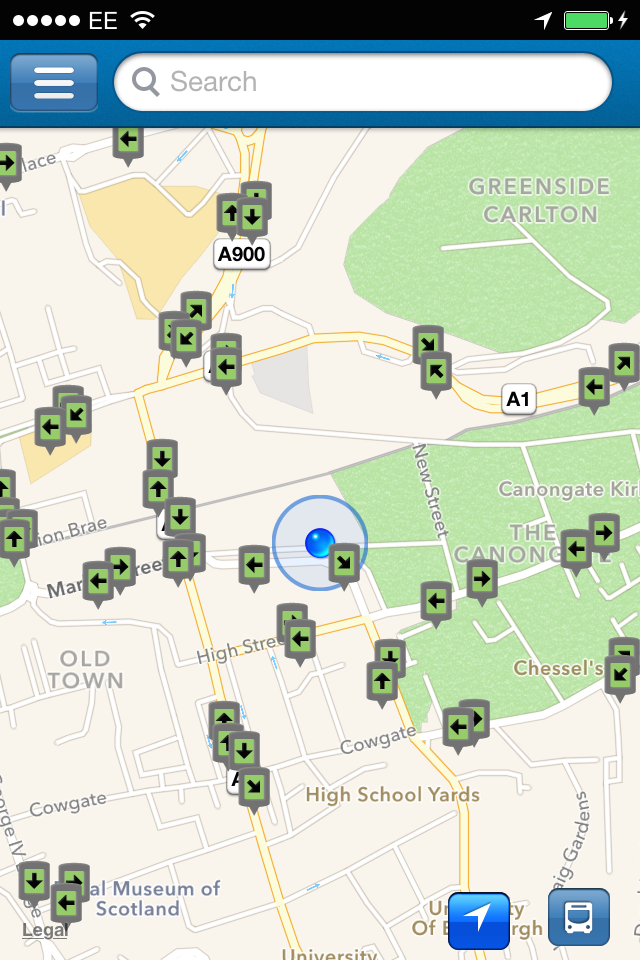
\includegraphics[width=\textwidth]{edinbus}
                \caption{A screen shot of the home screen of the Edinbus app}
                \label{fig:edinbus}
        \end{subfigure}
        \hfill
        \begin{subfigure}[b]{0.4\textwidth}
                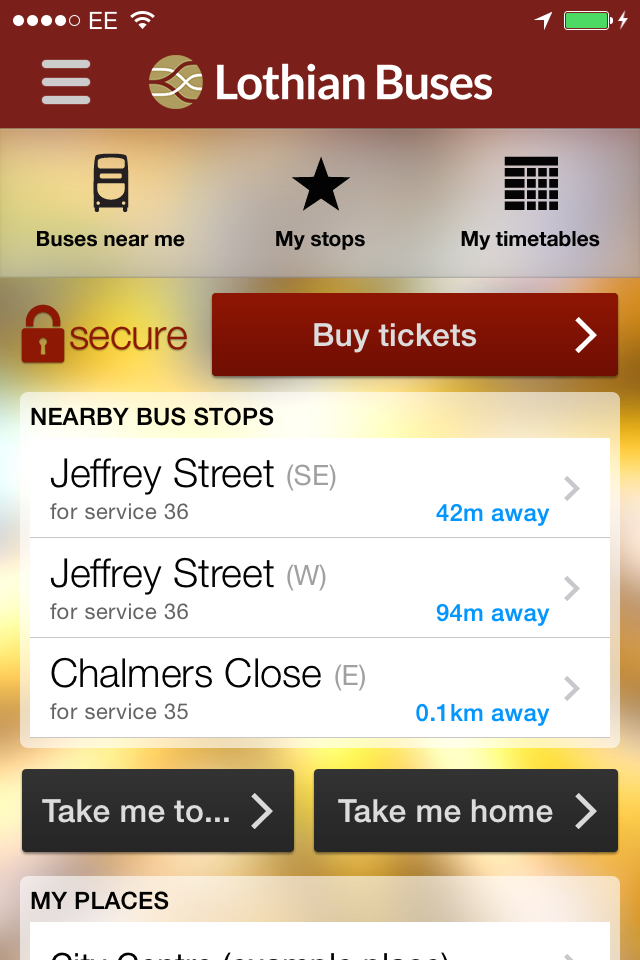
\includegraphics[width=\textwidth]{lothian}
                \caption{A screen shot of the home screen of the Lothian Buses Official App}
                \label{fig:lothian}
        \end{subfigure}
\end{figure}

The Lothian Buses official app was eventually used during the summative evaluation (in Chapter \ref{sec:summ}), so that the Talking Buses app could be evaluated against another bus travel utility app.

\subsubsection{Mexico City - Metrobus}
There are also several applications designed specifically to aid blind and partially-sighted users with bus travel. One such solution was "a mobile assistant to spatially locate and orient passengers of a Metrobus system in the city of Mexico" \citep{metrobus}. This solution involved several components, including a third generation (3G) mobile phone and separate GPS and compass devices, and was designed to identify the user's current location within the bus stations, and provide assistance in the form of audio-based information depending on the user's task. Tasks included orienting the user toward the exit or a specific gate using 'clock' directions (for example, "The exit is at five o'clock").

The research concluded that users found the instructions given "relatively precise" \citep{metrobus}, but in some cases GPS inaccuracy negatively affected the system's performance. Additionally, the usage of external positioning and communications hardware reduced the battery life of the mobile phone by 50\%. Despite this, users found that the system "gave them a better sense of security and confidence during their behaviour, also contributing to their overall navigation performance".

While GPS can be used to provide navigation assistance to blind and partially-sighted bus users, care will need to be taken in the Talking Buses app to ensure that poor location accuracy does not impair the quality of service offered.

\subsubsection{React Talking Bus Stops}
React is a system designed to aid independently mobile blind or partially-sighted people with navigation using "Talking Signs", \citep{react} - signs which dictate navigation information when a user passes by who is holding a "Trigger fob" (a battery-powered pocket-sized device which "sends a constant radio signal that is picked up by the RNIB React speaker unit" \citep{reactEdinburgh}). The trigger fob is asymmetrically shaped to help the user determine the correct orientation, and has two buttons used to communicate with the RNIB React sign.

A case study announced in 2007 resulted in the placement of 47 RNIB React signs in six train stations near Edinburgh and Glasgow \citep{scotrail}.  In addition, Edinburgh Council installed an RNIB React sign with real-time bus information at the Royal Blind School in Edinburgh, as part of a trial by RNIB \citep{royalBlindSchoolReact}.

Although responses to React have been positive \citep{reactEdinburgh}, and it is an example of a solution to aid with bus travel for blind and partially-sighted users, it is limited to providing assistance to users who are already located at the bus stop.

There are many reasons why a bus traveller may wish to investigate or plan their route before leaving their home, and this applies especially to blind and partially-sighted users \citep{stopForMe}. This limitation does not apply to Talking Buses, however, as it has access to an internet connection wherever the user is located.

Additionally, we wished to produce a solution which does not require any additional devices or hardware (such as the React trigger fob), which has been determined to be possible using smartphone technology.

\subsubsection{Scot Talk}
Released in late 2013, Scot Talk is an app produced by Traveline Scotland, designed to assist blind and partially-sighted bus users who use VoiceOver. The iPhone app allows users to locate nearby bus stops, save favourite bus stops, and track the bus's route once they are on board \citep{scottalk}.

During our investigation, the Scot Talk app did not appear to offer the level of reliability we aimed to achieve in providing information to the user - for example, loading departures from bus stops often failed to return any departures for busy bus stops during rush hour. This is presumably due to the app's relatively early stage in development.

Additionally, the Scot Talk app does not appear to have been designed to support partially-sighted users. Much of the text used in the app has too small a font size to be easily read by a user who is partially-sighted. Additionally, colour contrast between text (blue) and the background (white) could be increased.

\subsection{iOS mobile operating system}
For reasons identified during the Design phase, iOS was chosen as the smartphone platform that the Talking Buses app would be implemented on. In this subsection, we give an overview of the accessibility features offered by iOS.

\subsubsection{iOS Accessibility}
\label{sec:iosAccessibility}
As the capabilities of modern smartphones improve, several technologies have been created specifically to ensure they remain accessible to all users. Apple's mobile operating system, iOS, has a number of features built into it intended to aid blind and partially-sighted users:
\begin{easylist}
& \textbf{VoiceOver}: Allows an iOS device to act as a screen-reader, providing vocal descriptions of the user interface and the values of text areas on the screen. 
&& Developers can use this feature by annotating user interfaces with accessibility information, allowing blind or partially-sighted users to explore on-screen elements by dragging their finger over them. 
&& Arbitrary text can also be passed directly to VoiceOver to be dictated immediately. This can be useful for making announcements to the user which are not directly driven by user-interaction.
& \textbf{Zoom}: Allows the user to zoom in on an area on the screen by double-tapping with three fingers. Users can move the zoomed area around the screen, and can view the user interface at up to 500\% magnification.
& \textbf{Large Text}: Allows partially-sighted users to take advantage of larger fonts in specific Apple-made apps.
& \textbf{White on Black}: Allows for the reversal of colour of all content on the screen, allowing for increased contrast in certain situations.
& \textbf{Screen Curtain}: By quadruple-tapping on the screen using three fingers, a user can activate Screen Curtain, a feature which deactivates the display of the device. For some blind or partially-sighted users who use VoiceOver, this does not hinder their interaction with the device, and has the effect of prolonging battery life.
& \textbf{Invert Colours}: Users can choose to invert the colours on the display, which can improve readability of text for partially-sighted users.
& \textbf{Bold Text}: This setting causes certain text labels throughout the operating system to be displayed with a bold font weight.
& \textbf{Button Shapes}: One criticism of the minimal visual design of iOS 7 from an accessibility standpoint is the lack of definition of button elements. This setting causes a background to be drawn for button elements, increasing their visibility for partially-sighted users.
\end{easylist}

Because the Talking Buses app uses VoiceOver extensively to provide bus service information to blind and partially-sighted users, we now provide more details on its usage. Users learn a series of simple, generally intuitive gestures to direct VoiceOver \citep{voGestures}. We now detail some of these gestures.
\begin{easylist}[itemize]
& \textbf{Tap}: Selects a user-interface element and dictates a description of it.
& \textbf{Double-Tap}: Activates the selected element.
& \textbf{Swipe right}: Selects the next element (moving left-to-right, top-to-bottom).
& \textbf{Swipe left}: Selects the previous element.
& \textbf{Two-finger tap}: Stops VoiceOver's current dictation.
& \textbf{Two-finger swipe up}: Dictates everything on the screen, starting from the top.
& \textbf{Two-finger swipe down}: Dictates everything on the screen, starting from the current selected element.
\end{easylist}

There are also other gestures used to configure aspects of VoiceOver, such as the rate of speech and which voice is used for dictation.

When navigating between user-interface elements, there are two main options available to VoiceOver users. Some users explore a user interface by using the left and right swiping gesture, taking in information from left-to-right, top-to-bottom. Other users explore by dragging their finger over the screen, having VoiceOver dictate elements as their finger moves across them. This allows users to choose between exploring a user interface as a one-dimensional list, or as a two-dimensional space.

During testing with RNIB's Mobile User Group (described in Section \ref{sec:coopEval}), group members varied in their usage of VoiceOver: some used swipe gestures, some explored by dragging a finger, many used either strategy depending on the app in question, or their level of past experience with the user interface.

\subsection{Bus Service Information}
In order for a smartphone-based solution to provide users with real-time bus service information, it will be necessary to fetch information from one or more remote services. Fortunately, many cities and transport authorities are now creating public APIs, allowing developers to create products and services which utilise the information available. Here, we are specifically concerned with bus services in the city of Edinburgh.

\subsubsection{MyBusTracker}
MyBusTracker is a service managed by Edinburgh City Council, in collaboration with Lothian Buses, to provide up-to-date bus timetable information. The MyBusTracker API allows registered developers to query a central service for information on bus stops, the bus routes which service those stops, and the departure times of buses at a particular stop. 

This has been used by several third-party developers to build travel/utility apps, such as Edinbus for iOS or My Bus Edinburgh for the Android platform.  The MyBusTracker API can provide data in either JSON or XML format. Some of the information provided is real-time, for example, arrival times of buses; other information is updated weekly, for example, information on bus stops in the MyBusTracker system.

We outline the main methods offered by the MyBusTracker API:
\begin{easylist}
& \textbf{getTopoID} - The MyBusTracker database has a topology ID, an alphanumeric identifier which changes each time the MyBusTracker database is updated.
&& This is used by the server component to ascertain whether or not the Talking Buses database should be updated, minimising unnecessary load on the MyBusTracker API.
&& The topology ID is also used by the iOS app component to determine whether or not it needs to update its own local database.
& \textbf{getBusStops} - Provides information on the bus stops in the MyBusTracker system, including: bus stop name, heading (the direction in which buses leaving the stop travel), latitude and longitude.
& \textbf{getServices} - Provides information on bus services in the MyBusTracker system. This information includes the service mnemonic (an alphanumeric reference for the bus service, displayed on buses), the service name, and the eventual destination.
& \textbf{getDests} - Provides information on destinations in the MyBusTracker system, including their direction (whether the service is departing from or returning to the terminus), which services call at these destinations, and the destination name.
& \textbf{getBusTimes} - Provides real-time information on which bus services will call at a given bus stop and the estimated time of arrival in minutes for each incoming service.
& \textbf{getJourneyTimes} - Provides real-time information on the bus stops a particular bus service will stop at, and the estimated time until each bus stop is reached in minutes.
\end{easylist}

The getBusStops, getServices and getDests API methods are intended to be invoked periodically and the results cached - the information returned by these services will have changed only if the topology ID has updated. The data returned from these services will be stored in a database downloaded periodically by the app.

The getJourneyTimes and getBusTimes methods return real-time information, and can be invoked as often as is required. This information will be requested in real time directly from the app.

\subsubsection{National Public Transport Access Node - NaPTAN}
\label{sec:myBusTrackerLimitations}
One disadvantage of the MyBusTracker API is that bus stop names are always shortened or truncated to eleven characters, producing inaccurate bus stop names such as "Commonwlth Pool". This would be inconvenient for any developer attempting to provide a user with high-quality travel information, but if these bus stop names are to be dictated to the user using software, the length limitation could produce frustrating and unpredictable results.

Additionally, there are bus stops for which the name of the bus stop printed on the sign differs from the one provided by the MyBusTracker API. If a blind or partially-sighted user attempts to confirm their location by asking a sighted person the name of the bus stop, they may be confused by the conflicting information and assume that the app in use was not functioning correctly.

In order to solve these problems, a second source of bus service information was used. The NaPTAN database is "a UK nationwide system for uniquely identifying all the points of access to public transport in the UK".

The bus stop names provided by the NaPTAN database appear to be more closely aligned with those printed on bus stop signs in the real world. This means such disagreement between information provided in the "real world" and the "virtual world" can be kept to a minimum, improving the user's experience.

Additionally, the MyBusTracker API keeps no record of which streets bus stops are located on. This information could be very useful for a blind or partially-sighted bus user who has alighted from a bus service in an unfamiliar place.

The NaPTAN database was added during the first iteration on the functionality and design of the Talking Buses app, and the details of this integration are included in that subsection (Section \ref{sec:naptanImp}).


\section{Design}
In this chapter, we give a detailed overview of the process of designing a solution to the issues identified in the previous chapter. We give an insight on decisions made regarding system architecture and a choice of mobile operating system for the smartphone app. Finally the process of forming the intended functionality and design of the app is described.

\subsection{System Architecture}
From the early stages of the project, it was clear that a comprehensive solution would involve the implementation of two components:
\begin{easylist}[enumerate]
& A smartphone application capable of requesting and displaying real-time bus information from a remote location.
& A server application capable of storing and updating bus service information and delivering it to the mobile application.
\end{easylist}

Arguably, it would be possible to create a technology-based solution to aid with bus travel \textit{without} a server component - the mobile application \textit{could} handle all of the responsibility of fetching and parsing bus service information from remote sources. However, this was eventually decided against for the following reasons:
\begin{easylist}[enumerate]
& Performance: A non-negligible amount of data must be downloaded, extracted and parsed in order for the app to provide the necessary information to the user - a process which takes around 40 seconds to complete. Rather than this significant delay and network usage affecting each user of the app, it makes sense to do the bulk of the processing in one place, and pass the processed, concise results to each user. This has the effect of increasing the overall performance of the system, as the overall workload is minimised.
& API usage recommendation: An examination of the MyBusTracker API revealed the following usage recommendation: \textit{"it is strongly recommended to use a local cache in your application to avoid irrelevant access to the web server"}. This allows multiple developers to create products/services utilising the MyBusTracker API while keeping unnecessary load on the service to a minimum.
\end{easylist}

\begin{figure}[h!]
  \centering
    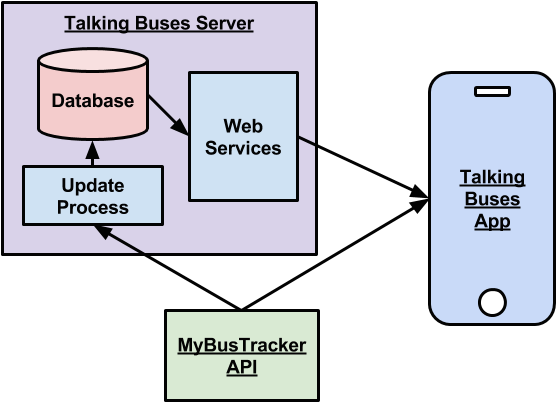
\includegraphics[width=0.7\textwidth]{sysArc}
    \caption{A diagram showing the initial system architecture of the Talking Buses app}
\end{figure}

\subsection{Choice of Mobile Operating System: Why iOS?}
Another decision made early in the design phase was the choice of mobile operating system to build the Talking Buses app for. When the design phase began in 2013, the most popular mobile operating systems for blind and visually impaired users were Apple's iOS (for iPhone, iPod Touch and iPad), and Google's Android (which runs on a wide variety of devices).

In late 2012, when this design decision was made, Research In Motion's Blackberry operating system was still a popular smartphone choice. However, it had little support for accessibility and so was not considered as a viable platform for this project. Windows Phone was also briefly considered, but it's market share was, at the time, prohibitively low (in late 2012, Windows Phone had only 5\% market share, compared to iPhone's 48\% \citep{marketShare}). 

As detailed earlier (in Section \ref{sec:iosAccessibility}), iOS contains a variety of features intended to make it more accessible to blind and partially-sighted users.

In late 2011, Google released version 4.0 of the Android mobile operating system, nicknamed "Ice Cream Sandwich". Ice Cream Sandwich introduced an "explore-by-touch" mode \citep{iceCream}, with similar functionality to that of iOS's VoiceOver (which had been present since iOS version 3.0, released mid-2009 \citep{ios3}). However, when the design phase of the project began in late 2013, adoption of Ice Cream Sandwich among Android users had only reached 30\% \citep{androidDistribution}.

At the time of writing, 20\% of Android users are still using a version of the operating system which does not have this vital accessibility functionality \citep{androidVersions}, whereas 97\% of iOS users use a version of the operating system released in the last 18 months \citep{appleDistribution}.

The accessibility features provided on iOS contribute to Apple's reputation for accessibility. As expressed by Stevie Wonder:
\blockquote{There's nothing on the iPhone or iPad that you can do that I can't do. As a matter of fact, I can be talking to you, you can be looking at me, and I can be doing whatever I need to do and you don't even know what I'm doing!} \citep{wonder}.

The popularity of iOS among members of the blind and partially-sighted community was also illustrated when meeting with RNIB's Mobile User Group - of the 12 blind or partially-sighted smartphone users, eleven of them owned iPhones and one owned an Android device.

\subsection{Functionality}
\label{sec:functionality}
In order to begin specifying the functionality of the app, we first consider a \textit{typical} use of bus transportation, and attempt to break it down into stages. Here, we use the term "user" to refer to a user of the bus service (as opposed to a user of the Talking Buses app).

\begin{easylist}[enumerate]
& Planning: The user ascertains (or is already aware of):
&& which bus services call at bus stops near the destination, and
&& which bus stops near the user are called at by these bus services.
& Navigation: The user navigates to an appropriate nearby bus stop.
& Waiting For Bus Arrival: The user waits for a particular bus service (or potentially one of several services), and boards it when it arrives.
& Waiting to Reach Bus Stop: The user waits for the service to reach the bus stop they intend to alight at.
& Alighting and Navigation: When the bus stop closest to the user's destination is reached, the user informs the driver, waits for the bus to stop and alights from the service. They then gain an understanding of their whereabouts and surroundings.
\end{easylist}

We then consider our target user, and based on the results of the literature review identify potential issues that blind and partially-sighted users potentially face at each of these stages. By identifying issues with each stage, the necessary and desirable functionality of the Talking Buses app is more easily recognised. We now consider each stage in more depth, detailing for each the potential issues faced, and potential functionality designed to mitigate or resolve these issues.

\textbf{1. Planning}:
Bus service information may be less accessible to blind or partially-sighted users. For example, timetables printed on leaflets or situated in bus stops are completely inaccessible if the user is travelling independently and there is no-one available to ask for assistance. Websites providing information as dense and complex as timetables for several hundred bus services often have accessibility issues when used with screen readers or dictation software.

\textbf{2. Navigation}:
Once the user has identified the bus stop they intend to depart from, they must navigate to the bus stop. While navigation has been identified as an area which blind and partially-sighted people may find challenging, providing general navigation assistance, for example in the form of turn-by-turn directions spoken to the user, was deemed to be outside the scope of the project, and there is already a great body of work in this area (as identified in Section \ref{sec:navAssistance}).

For example, blind and partially-sighted users can utilise directions provided by Apple's build-in Maps application, or use an external navigation assistance solution such as the Trekker Breeze in conjunction with the Talking Buses app.

However, there are many situations where little or no planning can take place before a user's journey, for example when the user needs to return home from an unfamiliar location. For this reason, it was thought to be essential to allow users to identify bus stops in their location, and access a range of information on their location and which bus services they are served by. In the example above, this allows users to ascertain which bus stops near them are suitable for their intended journey.

One challenging aspect of the information given by the MyBusTracker API is that bus stops located on opposite sides of a road are often named in pairs. Indeed, of the 2722 bus stops contained in the MyBusTracker system, over 900 of them share names with other bus stops. In order to mitigate the ambiguity this could cause, the Talking Buses app will provide a spoken representation of the heading of bus services leaving the bus stop.

\textbf{3. Waiting for Bus Arrival}:
When waiting for a desired bus to arrive at a bus stop, there are a number of challenges for blind and partially-sighted users. For example, bus users waiting at a bus stop are generally expected to be able to see the service number and destination of approaching buses to ascertain whether or not they intend to board, and should therefore signal to the bus driver indicating so.

For a blind or partially-sighted user, this can be a challenging or even impossible task. For this reason, the Talking Buses app will allow users to select a desired bus service while waiting at a bus stop, and receive regular spoken notifications on the estimated arrival time of the bus.

\textbf{4. Waiting to Reach Bus Stop}:
Once the passenger's bus has arrived, and they have boarded it, they must wait for the bus to reach a specific, desired bus stop before alerting the driver and alighting from the bus. However, if the passenger is blind or partially-sighted, many of the cues passengers usually use to successfully gauge their current whereabouts may be unavailable. This makes it difficult to ensure that they do not miss their bus stop, or alight from the bus too soon.

In order to address this, the Talking Buses app will provide a list of the bus stops that the service will call at on its route, giving estimated arrival times for each of the stops. This information will be regularly updated and will allow the user to gauge their whereabouts and simplify the process of judging when to alight from the bus service.

\textbf{5. Alighting and Navigation}:
Finally, the passenger alights from the bus service at a bus stop. For blind and partially-sighted bus users, orientation and exploration of the area can be challenging, especially if the bus stop is unfamiliar. Additionally, once the passenger has alighted from the bus, there may be nobody at the bus stop to offer assistance.

To address this, the Talking Buses app will provide the user with the name of the bus stop at which they have alighted from the service and the direction the bus was facing as it departed from the stop. This will allow users to gain an initial understanding of their surroundings.

Having examined the common sequence of events involved in bus travel, as well as issues our intended users potentially face in completing the required tasks, it became possible to define the app's intended functionality in terms of use cases (Section \ref{sec:iSimEval}).

\subsubsection{Functional Requirements - iOS app}
Based on the challenges identified, use cases created, and bus service information available, an initial functional specification was produced, detailing what information the app should provide at different stages of the user's bus travel.

When navigating to a bus stop:
\begin{easylist}[itemize]
& The user can find bus stops near their current location.
&& For each stop, the app should provide the bus stop name, its heading, and the current distance from the user in metres.
\end{easylist}

When waiting at a bus stop:
\begin{easylist}
& The user can check the bus times at nearby bus stops.
&& For each incoming bus service, the app should provide the bus service mnemonic, destination, and the estimated time(s) of arrival.
& The user can be alerted when the bus is due to arrive.
\end{easylist}

When travelling on-board a bus service:
\begin{easylist}
& The user can get information on the stops that the bus is approaching.
&& For each bus stop, the app should provide the bus stop name, its heading, and the bus service's estimated time of arrival at the bus stop.
\end{easylist}

Having alighted from a bus service:
\begin{easylist}
& The user can request information on where they have alighted from the bus service.
&& The app should provide the name of the bus stop at which the user alighted from the service, the street the user is currently located at, and the heading the bus stop is facing.
\end{easylist}

\subsubsection{Functional Requirements - Server}
The server component is designed to serve the iOS application with bus service information on demand. Due to the nature of the MyBusTracker API, only some information will be stored and served by the Talking Buses server, the rest can be requested as-required from the MyBusTracker API.

To provide the necessary information, two main services are required:
\begin{easylist}[itemize]
& A service which provides a database of bus stops, and the services that call at each of them. This information is downloaded by the app, and used to locate nearby bus stops and present information about them to the user.
& A service which provides sufficient information for the app to decide if it must update its own database of bus stops (i.e. if the MyBusTracker API information has been updated).
\end{easylist}

\subsection{Non-functional Requirements}
\subsubsection{Bus Service information}
There are three main requirements for bus service information provided by the Talking Buses app:
\begin{easylist}[enumerate]
& \textbf{Suitable for Dictation} - Because the Talking Buses app is intended for use with blind and partially-sighted users, we must ensure that any information provided to the user can be dictated using VoiceOver without issue. For example, bus stop names provided by the MyBusTracker API are shortened (e.g. "Commonwlth Pool", "W of Lanark Road") or truncated (e.g. "Clerwood terminu", "Mountcastle Driv") to eleven characters. When bus stop names such as these are dictated by VoiceOver, they can produce confusing and often bizarre results.

An example of where this could be challenging is when conveying the heading of a bus stop to the user. The MyBusTracker API provides headings for each bus stop in the form of an integer value between 0 and 359, which are not hugely useful to the user. Instead, these headings will be translated into compass headings (for example, instead of "facing one hundred and forty-three degrees from north" we use "facing south east").
& \textbf{Regularly Updated} - There are many reasons why bus service information can change, such as the placement of new bus stops, or changes to the routes of services.  Attempts must be made to ensure that all bus information relayed to the user by the app is accurate i.e. up-to-date information. The server component is (eventually) responsible for processing and storing data from two sources: the MyBusTracker API and the NaPTAN database. It must do so in such a way that the database contains information which is refreshed frequently.
& \textbf{Consistency} - We aim to strive for consistency in the information provided by the app. By this we mean that any information supplied to the user is in a regular, and thus predictable, format. An example of where this requirement is valuable is when creating descriptions of bus stops: because information on bus stops is provided by two different sources, each supplying varying information (for example, NaPTAN provides street names for bus stops), or even conflicting information (both NaPTAN and MyBusTracker offer bus stop names, and the names given are often different). In this case, efforts must be made to ensure that each bus stop in the Talking Buses system has complete information (bus stop name, heading and street name).
\end{easylist}

\subsubsection{iOS App Position Accuracy}
In order for the app to provide contextually-useful information to the user, it will make use of the iPhone's built-in GPS hardware to establish a position for the user and provide information specific to that location. One example of this is providing a list of bus stops located close to the user.

GPS accuracy is known to suffer in built-up, urban environments \citep{gpsAccuracy}, due to signals "bouncing off large buildings" \citep{gpsCity}. One study even reported GPS as performing especially poorly on buses \citep{gpsFeasibility}. As the app is intended to be used in a city, efforts must be made to mitigate the effects this has on the app's functions, and the user's experience.

\subsection{Talking Buses App Design}
\label{sec:appDesign}
Because the app is intended to be used primarily by blind and partially-sighted bus users, extra care must be taken over the design of the app. Information intended for the user must be communicated:
\begin{easylist}[itemize]
& Non-visually for blind users. This information will be given in audio format, dictated using iOS's VoiceOver technology.
& Visually for partially-sighted users. A criteria of usability heuristics will be defined which meet the needs of a variety of forms of visual impairment (such as cataracts or glaucoma).
\end{easylist}

\subsubsection{Design Principles}
\label{principles}
In order to address potential usability issues for blind and partially-sighted users identified in the literature review, a number of design principles and associated guidelines were identified.  There are many available sources for design principles. Some are compiled by designers of mobile operating systems (such as Apple), some are intended to apply more generally (such as the Universal Design Principles). The most specific, comprehensive guidelines found were compiled by Funka Nu, an accessibility consultancy based in Sweden \citep{funkaNu}.

As the design needs of the project are multi-faceted, principles and associated guidelines were gathered from several sources to produce a more comprehensive list. We now review this list of design principles and guidelines used in the design of the Talking Buses app, with principles grouped depending on their source, and also consider examples of how these principles apply to this project.

\textbf{Universal Design Principles}
\begin{easylist}[itemize]
& Equitable Use - The design is useful and marketable to people with diverse abilities.
&& This means that any information provided visually by the Talking Buses app should also be provided non-visually, using VoiceOver. Additionally, text used within the app will be designed to mediate the effects of various visual impairments.
& Simple and Intuitive Use - Use of the design is easy to understand, regardless of the user's experience, knowledge, language skills, or current concentration level. 
&& Descriptions of user-interface elements passed to VoiceOver should be informative enough to effectively communicate to the user what the element is for, and the results of interacting with it. Additionally, all information dictated to the user should be in a format which is both concise, and easily understood.
& Perceptible Information - The design communicates necessary information effectively to the user, regardless of ambient conditions or the user's sensory abilities.
&& The same information should be provided in multiple formats (text and audio-based), to cater for a wider range of ability in vision in the user.
& Tolerance for Error - The design minimizes hazards and the adverse consequences of accidental or unintended actions.
&& It should be possible and simple to undo actions made by the user. For example, accidentally selecting the wrong bus stop from a list should have minimal cost in the user's completion of the task.
\end{easylist}

\textbf{Funka Nu's "Guidelines for the development of accessible mobile interfaces"}
\begin{easylist}[itemize]
& Position important things higher up and less important things lower down.
&& When using VoiceOver, this principle especially applies to lists of information, where care will be taken to sort information in a way that makes sense given the context to minimise unnecessary action from the user where possible. For example, when the user is searching for nearby bus stops, they should be presented from closest to furthest away from the user.
& Strive for a clean design, and minimise unnecessary elements.
&& Care will be taken to ensure that every user interface element has a purpose, such that visual distraction is kept to a minimum.
& Create large tappable areas.
&& Table rows and buttons used in the design of the Talking Buses app will be large enough to be easily targeted and tapped by the user, or targeted using VoiceOver.
& Limit the quantity of information and the number of objects displayed.
&& Care will be taken to ensure that lists of information provided by the Talking Buses app are not overwhelmingly long. Through user testing, a suitable number of items will be displayed depending on the type of information.
& Use high contrasts.
&& All text displayed in the app will either be black on a white background, or vice versa, in order to maximise contrasts and make information as legible as possible for the user.
& Use simple navigation concepts.
&& Navigation between different functionality of the app will be as simple and intuitive as possible.
& Minimise text input in the user interface.
&& The app will be designed to keep text input from the user to an absolute minimum. In cases where text entry is necessary, dictation is offered by the iOS mobile operating system.
& Be consistent.
&& The layout and logic of each user interface presented to the user will be as consistent as possible. For example, "Back" navigation buttons will always appear at the top left of the screen, and user actions on user interface elements (such as selecting a row in a table) will have the same result each time (in this case loading a new view with information on the item in the selected row).
\end{easylist}

\textbf{Accessibility Programming Guide for iOS}:
In order to make bus service information accessible to blind and partially-sighted users, we take advantage of Apple's VoiceOver technology. This allows the user to explore the user interface using a series of gestures and have bus-service information dictated to them by the app. Care must be taken to ensure that various accessibility properties of user interface elements are set according to Apple's standards and constraints.

Apple have published a series of guidelines on the creation of suitable values for these attributes \citep{appleVOGuidelines}.  The guidelines provide two high-level requirements for accessible iOS apps:
\begin{easylist}[enumerate]
& all user interface elements are accessible (i.e. supply accessibility information for VoiceOver to dictate when focused on), and
& all accessibility information provided is helpful and accurate.
\end{easylist}

For each user interface element, there are four accessibility attributes which can be configured: the element's value, label, hint, and traits. We now summarise the guidelines given for creating sensible VoiceOver attribute values for each.

\begin{easylist}[itemize]
& The value attribute is intended to give a summary of the current value of the element. The method of doing so will depend on the type of element. For a UITextLabel, the label's contents should be used (and, if necessary, adapted for dictation). For UIImageView (a container for displaying an image), a text-based description of the image should be provided. For other types of element the value attribute is less intuitive - for example, for a UISlider element (designed to allow smooth, continuous adjustments to a variable), the description of the value will depend on the variable being adjusted, and the unit of measurement used in the description (screen brightness is expressed as a percentage, whereas a user's rating of arbitrary content may be measured using a number of "stars" out of five).
& The purpose of the label attribute is to "identify the user interface element" \citep{appleVOGuidelines} to the user. This often involves supplying the same or similar information a non-VoiceOver user can infer from the element by looking at it. To this end, Apple suggest that the label value be brief (ideally a single word or short phrase), begins with a capitalised word (to aid with VoiceOver's pronunciation), and does not contain the type of the user interface element, as VoiceOver already dictates this (for example, if a button's accessibility label is set to "Refresh button", VoiceOver will dictate "Refresh button button", because it is a button whose label is "Refresh Button").
& The hint attribute is used to give the user a description of what will happen if they interact with the element in question. The hint attribute of an element should only be used when the results of interacting with it are not immediately clear from the label property or its context, as this keeps unnecessary information "clutter" to a minimum for the user. The hint should describe the result of interaction as concisely as possible, beginning with a capitalised verb and ending with a full stop. It should not include the name or type of the element, or the name of the expected gesture (i.e "Deletes the item" is more suitable than "Double-tap to delete the item"), as these are likely to be included in VoiceOver's description of the element.

Interestingly, VoiceOver can be configured by the user not to read hints. This is generally done by experienced VoiceOver users who require less information (as confirmed by several members of the Mobile User Group of RNIB). For this reason, attempts will be made to avoid placing crucial information in the hint attribute of user-interface elements.
& Finally, Apple provides guidance on the use of traits. One or more traits are applied to an element to concisely describe its type or behaviour to the user. Examples of pre-defined traits include Button, Updates Frequently, Plays Sound and Selected. Apple suggests using one "type" trait (e.g Button) and one "behaviour" trait (e.g. Not Enabled) to describe each element.
\end{easylist}

When focus is given to a user-interface element, VoiceOver first reads the element's label, then its value, then its list of traits, then finally, and unless the user has disabled hints) the element's hint. To illustrate this, we provide an example: the refresh button present on the Nearby Buses screen. Because the refresh button is an instance of a system-defined user-interface element, some of these accessibility properties are already suitably set and therefore are left unmodified.
\begin{easylist}[itemize]
& The refresh button's label attribute is already appropriately set to "Refresh", and so is not modified.
& As the refresh button has no obvious value or state (it does not toggle, for example), the value attribute is left blank.
& The hint attribute is empty by default, and is therefore programmatically set to "Reloads nearby bus stops", providing a description of the result of interacting with the button to the user where it could potentially be unclear.
& The single predefined trait for the element is "Button". This is suitable, and gives the user a good idea of what types of interaction are available.
\end{easylist}

For this element, VoiceOver's spoken description would be:
\begin{quote}
"Refresh. Button. Reloads nearby bus stops."
\end{quote}
This short message takes around three seconds to dictate, and tells the user everything they need to know about the element: what it is, how it behaves, and the results of the user's interaction.

The guidelines described above will be followed  when considering how VoiceOver would be applied in the Talking Buses app.

\subsubsection{Visual Design}
It could be argued that visual design is a less important aspect of a project intended for blind and partially-sighted users. However, there are many aspects of visual design that will be crucial in allowing partially-sighted users to interact with the app, and in allowing blind users to leverage VoiceOver effectively. We review these aspects below.

As identified during our investigation of visual impairments and their manifestation in visual perception, reading text can be a challenging task for many partially-sighted people. For this reason, attention will be given to typography: the style and appearance of text used in the app.

Any text displayed to the user will have maximum contrast against the background (i.e. black text on white background), will have a bold font weight to increase legibility, and will be of as large a font size as possible depending on the context.

Layout concerns the placement and size of user interface elements on the screen and is an important aspect of the app's visual design. Alignment of elements can give the user an overview of a user interface at a glance. Elements such as text labels and buttons will be suitably aligned where possible to give the user an impression of the user interface layout even if the user lacks visual acuity. 

When a blind or visually-impaired user is using VoiceOver to explore a user interface, the ordering of elements can be especially important. If the user uses 'flick' gestures (dragging a single finger across the display of the device) to navigate between elements, the focus of VoiceOver will progress from left to right, progressing down the screen. As such, it is especially important to place important elements where they will be discovered with minimal effort. Important elements such as page headings or general controls will be placed at the top of the user interface.

Additionally, as partially-sighted users are often unable to understand the layout and logic of a user interface 'at a glance' (as sighted users are able to), care should be taken to ensure that ordering of elements is simple and intuitive.

A mockup of the initial design of the Nearby Stops screen in the app is provided to illustrate the visual design considerations outlined above. Points to note about this initial design are the following:
\begin{easylist}[itemize]
& The most important elements (the screen's heading and the refresh control) are located at the top of the screen.
& The text labels in the cells are aligned.
& All text is black on a white background, in a bold font.
\end{easylist}

\subsubsection{Interaction Design}
An interaction design was formed, detailing how users would progress through the functionality offered by the app in order to achieve their goal.  The app was split into five screens or stages, each intending to provide functionality for a specific part of the user's journey.  Once these screens were identified, as well as the information given by each of them, several options were considered as methods of transitioning between them.

Because the app is already accessing the user's position to locate nearby bus stops, we investigated attempting to use GPS information to infer the user's current method of transportation - whether walking, or travelling on a bus.  One 2012 paper attempted to accomplish this using GPS data collected in London, for various modes of transportation (car, walk, cycle, underground, train and bus). The method involved an approach based on Support Vector Machines and achieved 88\% classification accuracy \citep{infer}. While this paper was useful as a proof of concept, the method used seems too computationally expensive to be implemented on the iPhone without implications for battery life and overall performance.

Instead, on each screen in the Talking Buses app, intuitive user actions were identified for progressing to the next screen.  Frequently, the app communicates lists of information to the user (for example, lists of nearby bus stops, or lists of bus services due to arrive) and the user intends to do something relating to these list items (for example, selecting a nearby bus stop from which to board a bus service). In these cases, the user can simply select the list item to progress to the next screen.

Two of the five screens identified ("Waiting for the Bus" and "Off the Bus") could not be suitably adapted to fit this pattern, as they do not display lists of information to the user. On these screens, progression is achieved by the user by selecting buttons which are labelled according to their functionality (e.g. "Show Service Route").

On all screens identified (except the first), users can navigate back to the screen directly before using a back button at the upper-left corner of the user interface. The placement and functionality of this button is consistent with Apple's design principles, and so VoiceOver users will expect it. Additionally, it provides the user with a simple, consistent way to undo actions, such that any mistakes made (such as accidental selection of the wrong row in a table) can be undone easily.

There are refresh buttons on most screens of the app (on all except the screen displayed after the user has alighted from a bus service). These are used either to refresh the list of nearby bus stops (taking into account a more recent position update), or refreshing real-time information (such as arrival times of buses at a bus stop).  In addition, it was decided that these screens would refresh automatically on a frequent basis, allowing for the app's functionality to be used without interaction during certain tasks.

\begin{figure}[h!]
  \centering
    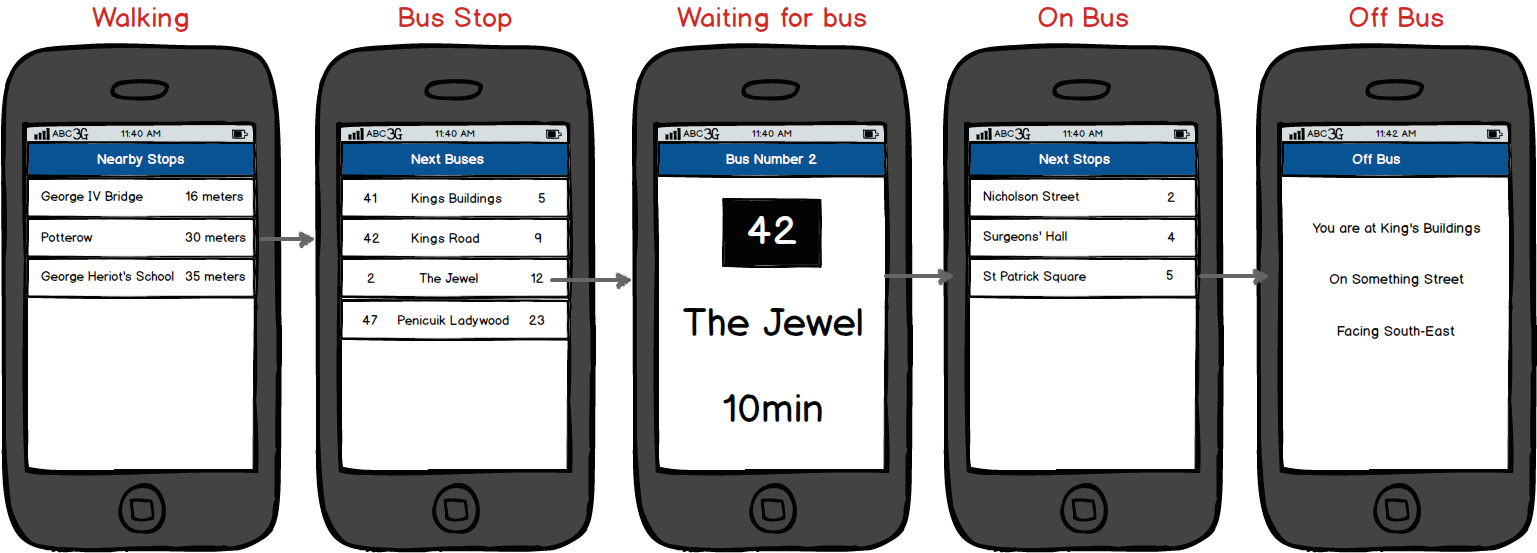
\includegraphics[width=\textwidth]{interaction}
    \caption{A diagram showing the initial interaction design of the Talking Buses app}
\end{figure}

The five screens identified are described below, detailing the information provided and potential actions performed by the user.
\begin{easylist}[enumerate]
& \textbf{Walking to the Bus Stop} - This screen provides the user with a list of nearby bus stops, giving the name, heading and the distance in metres for each of them. The user is able to select the bus stop they intend to use from the list, and progress to the next screen.
& \textbf{At the Bus Stop} - This screen presents the user with real-time information on bus services arriving at and departing from the bus stop that they selected in the previous screen, providing the service's mnemonic (e.g 44A), final destination and estimated time(s) of arrival. The user can select the bus service they intend to use in order to indicate this to the Talking Buses app. The user can also press the back button to return to the previous screen.
& \textbf{Waiting for the bus} - This screen provides the user with real-time updates of when the bus service which they have selected will arrive at the stop. The user will be provided with increasingly frequent updates as the bus service approaches. When the bus arrives, the user can inform the app that they have boarded the bus by pressing a button.  If the real-time bus information suggests that the bus has left the stop before this happens, the user is asked if they have boarded it. The user can also press the back button to return to the previous screen.
& \textbf{On the Bus} - This screen provides the user with real-time information on the bus journey. A list of the bus stops the service is approaching is provided to the user, each detailing the name and heading of the bus stop, as well as when the bus is expected to reach it. The user can select an item in this list to tell the app that they will alight from the bus service at this stop.  The user can also press the back button to return to the previous screen.
& \textbf{Off the Bus} - This screen provides the user with information on where they have alighted from the bus service, including the bus stop name, and its heading . The user can press a button to find nearby bus stops (if they intend to use another bus service), or go back to the previous screen as described above.
\end{easylist}

\section{Implementation}
In this chapter, we give details of the implementation of the Talking Buses system. We consider the server and iOS application components separately. 

\subsection{Server Component}
The server component needed to be hosted somewhere it could be reached by the iOS application. Rather than purchasing, configuring and maintaining server hardware, we take advantage of Amazon Web Services' (AWS) Elastic Compute Clouds (EC2) service.

EC2 offers "resizable compute capacity in the cloud" \citep{ec2}, providing developers with a virtualised instance to their specifications. Amazon offer a variety of different types of instance depending on the type of resource required (examples include Compute-optimized, GPU Instances, or Memory-optimised instances). The user of the service can select an operating system of their choice and pre-install commonly used software packages.

Given the relatively low computational requirements for the server component, a Micro-instance was deemed to suit the needs of the project. Additionally, Amazon offer a 12-month free trial for instances of this type, minimising the costs of the solution \citep{freeAWS}.  The instance was configured to use Ubuntu Server 12.04, as it was deemed to be suitable for running a wide variety of web server and database applications.

The instance was associated with an Elastic IP address, a service included in AWS which allows for quickly and programmatically remapping IP addresses to different instances \citep{elasticIP}. This IP address was then tied to a subdomain of a domain name record the developer already owned. This set-up allowed the iOS app component to reliably fetch bus service information from the server component using a known URL.

\subsubsection{Database}
It was decided that development would begin by analysing the format of information provided by the MyBusTracker API, and then deciding what information was relevant to the functionality of the Talking Buses app.  Information on the following was deemed suitable for fetching and storing on a regular basis:
\begin{easylist}[itemize]
& The MyBusTracker topology ID would be stored, in order to later determine if the information held by the MyBusTracker system had updated and so to cause the Talking Buses system to update. This information comes from the \textbf{getTopoID} of the MyBusTracker API.
& Information on Bus Stops would be stored, including the name of the bus stop, its latitude and longitude, and a heading indicating the direction in which buses leaving the stop travel. This information comes from MyBusTracker API's \textbf{getBusStops} method.
& Bus Service information was determined necessary to store, in order to inform passengers which services call at which bus stops. This information includes a service mnemonic, the name of the bus service, and the name of the destination, and comes from the MyBusTracker API \textbf{getServices} method.
\end{easylist}

It was decided that information on destinations did not need to be stored, as it is included with the real-time information returned by the MyBusTracker API when requesting information on incoming bus services for a specific bus stop.

The getBusStops method of the MyBusTracker API provides, for each bus stop, a list of the services which serve the bus stop. These are given as a list of identifiers which correspond to the identifiers returned by the getServices method. In order to represent this many-to-many relationship of bus stops to bus services, a lookup table was used. This will allow, for example, for fetching of the mnemonics of bus services which call at a particular bus stop (valuable information for our users).

A database schema was designed to store the information described above, shown in Figure \ref{fig:schema}, and this database design was implemented using MySQL, creating the database, its tables, and relationships between them using a series of MySQL queries.

\begin{figure}[h!]
  \centering
    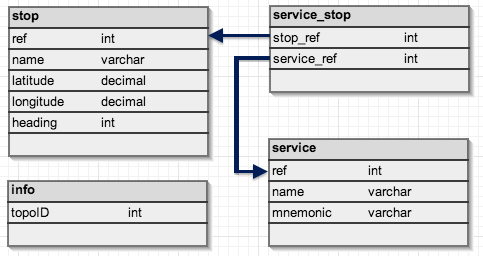
\includegraphics[width=0.8\textwidth]{schema}
    \caption{A visual representation of the initial database design}
    \label{fig:schema}
\end{figure}

\subsubsection{Integration with MyBusTracker API}
\label{sec:serverIntegration}
The service required a method of fetching information from the MyBusTracker API and storing it in the database designed in the previous subsection. In this subsection we give details on how this was achieved.

In order to request bus service information from the MyBusTracker API, developers must identify with the service by providing a key. This key is generated by producing the MD5 hash of the developer's API key concatenated with a current timestamp in Universal Time Coordinated (UTC) format. This key-creation functionality was implemented in Python.

Interaction with the API then takes the form of the server placing HTTP GET requests to various API methods (outlined earlier). The Python programming language was used to create a means of placing these requests, writing the results to a file, and then parsing the JSON data into Python dictionary objects. This process was generalised and implemented for each of the MyBusTracker API methods necessary for the Talking Buses system.

Lastly, these Python dictionaries are converted into MySQL insertion statements so they can be inserted into the Talking Buses database. As noted in the previous subsection, we are only interested in some fields of the objects returned by the MyBusTracker API, and these alone are extracted.

As mentioned before, we need a means of associating bus services with the stops that they serve. As each bus stop is processed by the system, the list of service references included are used to create rows in our service\_stops lookup table, storing this relationship.

\subsubsection{Web Services}
The server component is now capable of requesting and storing bus service information from the MyBusTracker API. However, it also needs to be capable of providing this information to the iPhone app when requested, by exposing a number of web services of its own.  There were deemed to be two web services necessary, and we now explore these.

\textbf{getTopoID}:

The first web service required provides the topology ID currently stored by the Talking Buses server component. This is used by the iPhone to determine if it must update its own locally-held information on bus stops. The implementation of this web service was relatively straightforward: a cgi-script is used to retrieve the topology ID stored by the Talking Buses database, and outputs this value. This web service is accessed by the iPhone application by placing an HTTP GET request to the URL at which the cgi-script is located.

\textbf{getBusStops}:

The second web service required provides the iPhone application with the list of bus stops currently stored in the Talking Buses database. Because we want to provide the user with a list of the service mnemonics of bus services which serve each bus stop, this web service performs several table joins before returning a result which includes concatenated values from other tables.

The following MySQL Query demonstrates this:
\begin{quote}
SELECT stop.name, GROUP\_CONCAT(service.mnemo) FROM stop\\
INNER JOIN stop\_service ON stop.ref = stop\_service.stop\_ref\\
INNER JOIN service ON stop\_service.service\_ref = service.ref\\
GROUP BY stop.name\\
\end{quote}

The query above returns the following results (using some arbitrary test data).
\begin{figure}[h!]
    \centering
    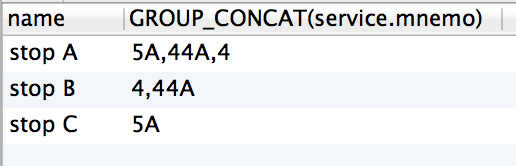
\includegraphics[width=0.5\textwidth]{join}
\end{figure}

The MySQL rows returned contain (for each bus stop) the bus stop name, latitude and longitude, heading, and the list of service mnemonics for bus services calling at the bus stop. These rows are encoded as JSON data, and then returned by the web service. This provides the iPhone app with a complete listing of bus stop information.

\subsection{iOS App Component}
\subsubsection{User Interface Implementation}

Much of the user interface of the iOS app was implemented using Interface Builder, a tool included in XCode for creating user interfaces in a visual, WYSIWYG manner. Interface Builder allows developers to drag user interface elements such as labels or buttons from a library onto a view. Various aspects of these elements can then be configured, such as fonts for text labels, or the size and appearance of a button.

While it is possible for developers to "draw in code" (that is, to build user interfaces by instantiating and configuring user interface elements in the application code, rather than using Interface Builder), it was decided that the WYSIWYG approach would be used where possible, allowing for rapid iteration on the user interface design, as the results of changes could be seen instantly (without waiting for the project to recompile, install, and open on the testing device).

The various accessibility attributes for user interface elements can be configured using Interface Builder. However, when these accessibility attributes are not "static", but vary depending on the properties of the objects they represent, it can be simpler to configure these attributes programmatically. To provide an example of this, we consider the way these attributes are defined for a table row representing a bus service which calls at a bus stop selected by the user.

In this case there are several aspects of the incoming bus service that the user may be interested in (including the mnemonic used to refer to the service, the service's destination, and estimated arrival times), and we must make an effort to provide all of this information to the user in an understandable but concise manner. The following format was selected:
\begin{easylist}[itemize]
& Label: "Number [mnemonic] bus."
& Value: "Arriving in [E.T.A] minutes, going to [destination]."
& Hint: "Provides updates of arrival times for this service."
\end{easylist}

When the user moves the VoiceOver cursor onto the table row, the following description is dictated (with the missing values filled):
\begin{quote}
\textit{"Number 36 Bus. Arriving in 5 minutes, going to Holyrood. Provides updates of arrival times for this service."}
\end{quote}

\subsubsection{Integration with Bus Service Information Services}

In order to provide bus service information to the user, the app had to be capable of downloading and interpreting data from two sources: the Talking Buses server component, and the MyBusTracker API. In both cases, the services return JSON data (with the exception of the Talking Buses getTopoID service, which simply returns a string).

To this end, a class was designed and implemented in Objective-C to handle the following functionality:
\begin{easylist}[itemize]
& placing HTTP requests to web services, when provided with the appropriate URL for the intended service,
& responding to errors with the request (including timeouts, and a lack of internet connectivity on the device), and
& decoding the response data into a string object
\end{easylist}

Subclasses of this class were then implemented for each service, responsible for:
\begin{easylist}[itemize]
& generating the URL for the request, depending on any fields which must be populated (for example, the key used for identification to the MyBusTracker API), and
& parsing the JSON response from the service into various objects, depending on which service is used.
\end{easylist}

Four of these subclasses were implemented, two for the Talking Buses web services (getTopoID and getBusStops), and two for the MyBusTracker API methods (getBusTimes and getJourneyTimes). This architecture allowed for a robust way of requesting bus service information, parsing the results and handling errors.

\subsubsection{Managing the Local Bus Stop Database}
When the user opens the app, it must immediately ensure that it has a locally-stored database of bus stops, and that this information is up-to-date. We now give details on this process, and consider its potential ramifications on performance for the user.

In order to rapidly implement a working prototype (to maximise the potential for user testing and iteration on the design and implementation), the initial solution used by the iPhone app to store bus stop information from the Talking Buses server component was as straightforward as possible. When the list of bus stops is received by the app, it is parsed from a JSON string into an array of NSDictionary objects (with the fields of each dictionary representing aspects of each bus stop).

This array of dictionaries is then serialised into a property list file and stored on the device. Property lists are a common method of creating a representation of an object which can easily be written to file. In this case, the property list files contained an array of dictionaries representing bus stops.

The same solution is used to store the topology ID of the local database of bus stops held by the Talking Buses app.

When opened, the app instantiates an instance of the subclass dedicated to fetching the current topology ID stored on the Talking Buses server. Once this ID is received, it is compared to the 
topology ID stored by the app. If the topology IDs are different, or the app does not have a stored topology ID (indicating that it does not have a database of stops), it proceeds to download new bus stops.

The app instantiates an instance of the subclass dedicated to downloading and parsing bus stop JSON data from the Talking Buses server component, and stores the bus stops in a property list as described above. The stored topology ID is also updated to the one returned by the server component earlier, to ensure the update process is not needlessly repeated the next time the app is opened.

Now, the app has ensured it has an up-to-date list of bus stops stored locally, and it can continue with normal execution: loading the contents of the file into an array of bus stops and locating those that are nearby.

Provided that the user has an internet connection, fetching the topology ID from the server component takes very little time (the response is only 32 bytes), as does comparing it to the topology ID stored by the app.

Fetching an initial or updated list of bus stops from the server involves downloading just under one megabyte of JSON data, and parsing it. Some basic testing indoors revealed that the app could do this in just under 5 seconds, not a prohibitive delay for the user.

\subsubsection{Finding the User's Location, and Nearby Bus Stops}
In order to locate nearby bus stops, the iPhone app will require access to the user's current location. For this, we use the CoreLocation framework, designed to provide mid-level access to position data. By instantiating a location manager and registering for location updates, a developer can define a method to be run each time the device receives a GPS update.

The developer can then access various properties of this location update, including the latitude and longitude, the accuracy of the GPS location (expressed in metres), and a timestamp representing the moment when the location update was received.

This location is then used by the app to locate bus stops near the user, and provide a distance in metres for each of them. This is done by iterating through each bus stop and calculating the distance to the device's current position. The bus stops are then sorted using this distance in ascending order (i.e. from closest to furthest from the user). Only a limited number of these nearby bus stops are displayed, so not to overwhelm the user with more information than is useful or necessary.

The CoreLocation framework also allows a developer to ascertain the horizontal accuracy of each location provided by the GPS hardware (as a number of metres). Setting a minimum tolerance for the accuracy of new locations will allow us to reject updates if they are likely to be incorrect. This is used to reject location updates which are not accurate enough to provide a desirable quality of service to the user.

\subsubsection{Fetching Real-time Bus Service Information}
There are two cases where real-time bus service information is required by the app: when providing departure times for bus services from a selected bus stop (which includes estimated departure times for each service), and when providing journey information for a specified bus service (which includes estimated arrival times at bus stops on the service's route).

As mentioned in an earlier subsection on implementation of the server component (Section \ref{sec:serverIntegration}), a key must be provided to identify the requestor to the MyBusTracker API when requesting information. This key generation process was implemented in Objective-C to allow for requesting of real-time bus service information directly from the iPhone app.

When requesting information on bus departure times using the MyBusTracker API method \textbf{getBusTimes}, we include two other values besides the key. The first of these provides the identifier for the bus stop the user has selected, and the second specifies the number of departures requested for each bus service serving the bus stop.

When the JSON response is received, it is parsed and the list of bus services (each containing a list of expected departure times for the service from the selected stop) is extracted. This information is then provided to the user, allowing them to effectively plan bus journeys.

Once the user has selected a bus service, they have the option of viewing the route of the service, including estimated arrival times for each stop on the route. This is accomplished by requesting information from the \textbf{getJourneyTimes} method of the MyBusTracker API. This request also requires parameters: the identifier for the bus stop the user has selected previously, and the identifier for the journey (essentially an instance of a bus service), which is included in the response from the \textbf{getBusTimes} method described above.

The response includes a list of bus stops that the bus service will serve, and an estimated arrival time for each (expressed as a number of minutes). This information is provided for the user, allowing them to track the progress of the bus while they are on it, and ensure that they alight from the service at their intended destination.


\section{Iteration}
In this chapter, details are provided on how the design and functionality of the Talking Buses system as described in the previous chapter evolved. Changes were largely made as the result of feedback received at a series of meetings with members of RNIB's Mobile User Group. Other changes were made to improving the implementation of various aspects of the iOS app and server components.

\subsection{Formative Evaluation}
In order to allow the design and functionality of the Talking Buses system to evolve in a direction which suited the needs of the users, a formative evaluation was conducted for the duration of the project. A formative evaluation is one which takes place throughout the duration of the project, with the aim of involving the users as early on in the project as possible, and then relying on their continued involvement for the duration of the project \citep{formativeEval}.

During the initial stages of the project (before implementation began) several investigations were made to inform design and functionality decisions. First, the MyBusTracker documentation was examined to see what information would be available at different stages of use of the app, and therefore what functionality could be offered to the users.

Next, a literature review was conducted to investigate the target users further, and identify accessibility concerns for mobile applications for these users. This review was used as the basis for most of the initial interaction and visual design decisions made. This review also identified difficulties that blind and partially-sighted users face in the domain of independent travel, and specifically while using bus services.

\subsubsection{Product Iteration}
Once a prototype had been produced, iteration on the design and functionality of the app was motivated by a series of meetings with members of the RNIB Mobile User Group, at the RNIB offices in Hillside Crescent, Edinburgh. During these meetings, group members had the opportunity to interact with the prototype, discuss any issues and suggest features.  These regular, informal evaluations provided valuable feedback on the app's progress, and allowed for an iterative development process.

The members of the RNIB Mobile User Group were very enthusiastic and encouraging about the work. They frequently reiterated the demand for the Talking Buses app, and provided valuable feedback and suggestions.

Several suggestions for functionality that were included in the final design include:
\begin{easylist}[itemize]
& the addition of street names to bus stop descriptions,
& a method of marking selected bus stops as favourites,
& a method of searching for bus stops by name or street name,
& grouping together bus arrival times by bus service number, instead of displaying the arrival time of each bus individually, and
& a method of adding frequently-used bus stops to a list of favourites.
\end{easylist}

Additionally, feedback was received on many design and accessibility issues, including:
\begin{easylist}
& the format of information dictated by VoiceOver to the user (such as the ordering of statements and acceptable abbreviations),
& ideal lengths for lists of information, such as nearby bus stops or incoming bus services, and
& sizes and fonts used for text in labels within the application (primarily intended for partially-sighted users).
\end{easylist}

\subsection{First Iteration}
The first iteration on the design and functionality of the Talking Buses app took place after the initial meeting with members of the RNIB Mobile User Group. At this time, a functional prototype had been developed, and the app had been made accessible, as described in the previous chapter. The feedback received during this meeting was both encouraging and valuable.

The meeting took place on October 9th, 2013, at the RNIB headquarters located in Edinburgh. Two members of the Mobile User Group attended, and were able to offer some valuable insights into difficulties faced by the blind and partially-sighted community, especially concerning bus travel.

Both attending members were legally blind, one had been without vision since birth. Both members were users of iOS products (both were iPhone owners) and familiar with VoiceOver technology. One of the members lived in Edinburgh and was a regular user of the bus services, the other lived outside Edinburgh but also used bus services regularly. Both members immediately identified themselves as potential users of the app.

During the meeting, they were given an opportunity to use the prototype and offer any feedback or suggestions for functionality. The following feedback was received:
\begin{easylist}[itemize]
& Reactions from both test users were positive and very encouraging. They both stated that there was much demand for the app, and one user described the experience of being able to check departure times for a bus stop several hundred metres away as "Absolutely wonderful!".
& Both users indicated that all of the functionality offered by the prototype was valuable in using bus services independently and "with confidence".
& Both test users indicated a desire for functionality allowing the user to mark frequently-used bus stops as being "Favourites". This would allow users to check departures at bus stops they were not currently located at.
& Both test users also suggested the addition of street name information to the descriptions of bus stops given. This would allow them to better orient themselves, and decide which bus stops were potential destinations more easily.
\end{easylist}

\begin{figure}[h]
    \begin{minipage}[b]{0.5\linewidth}
        \centering
        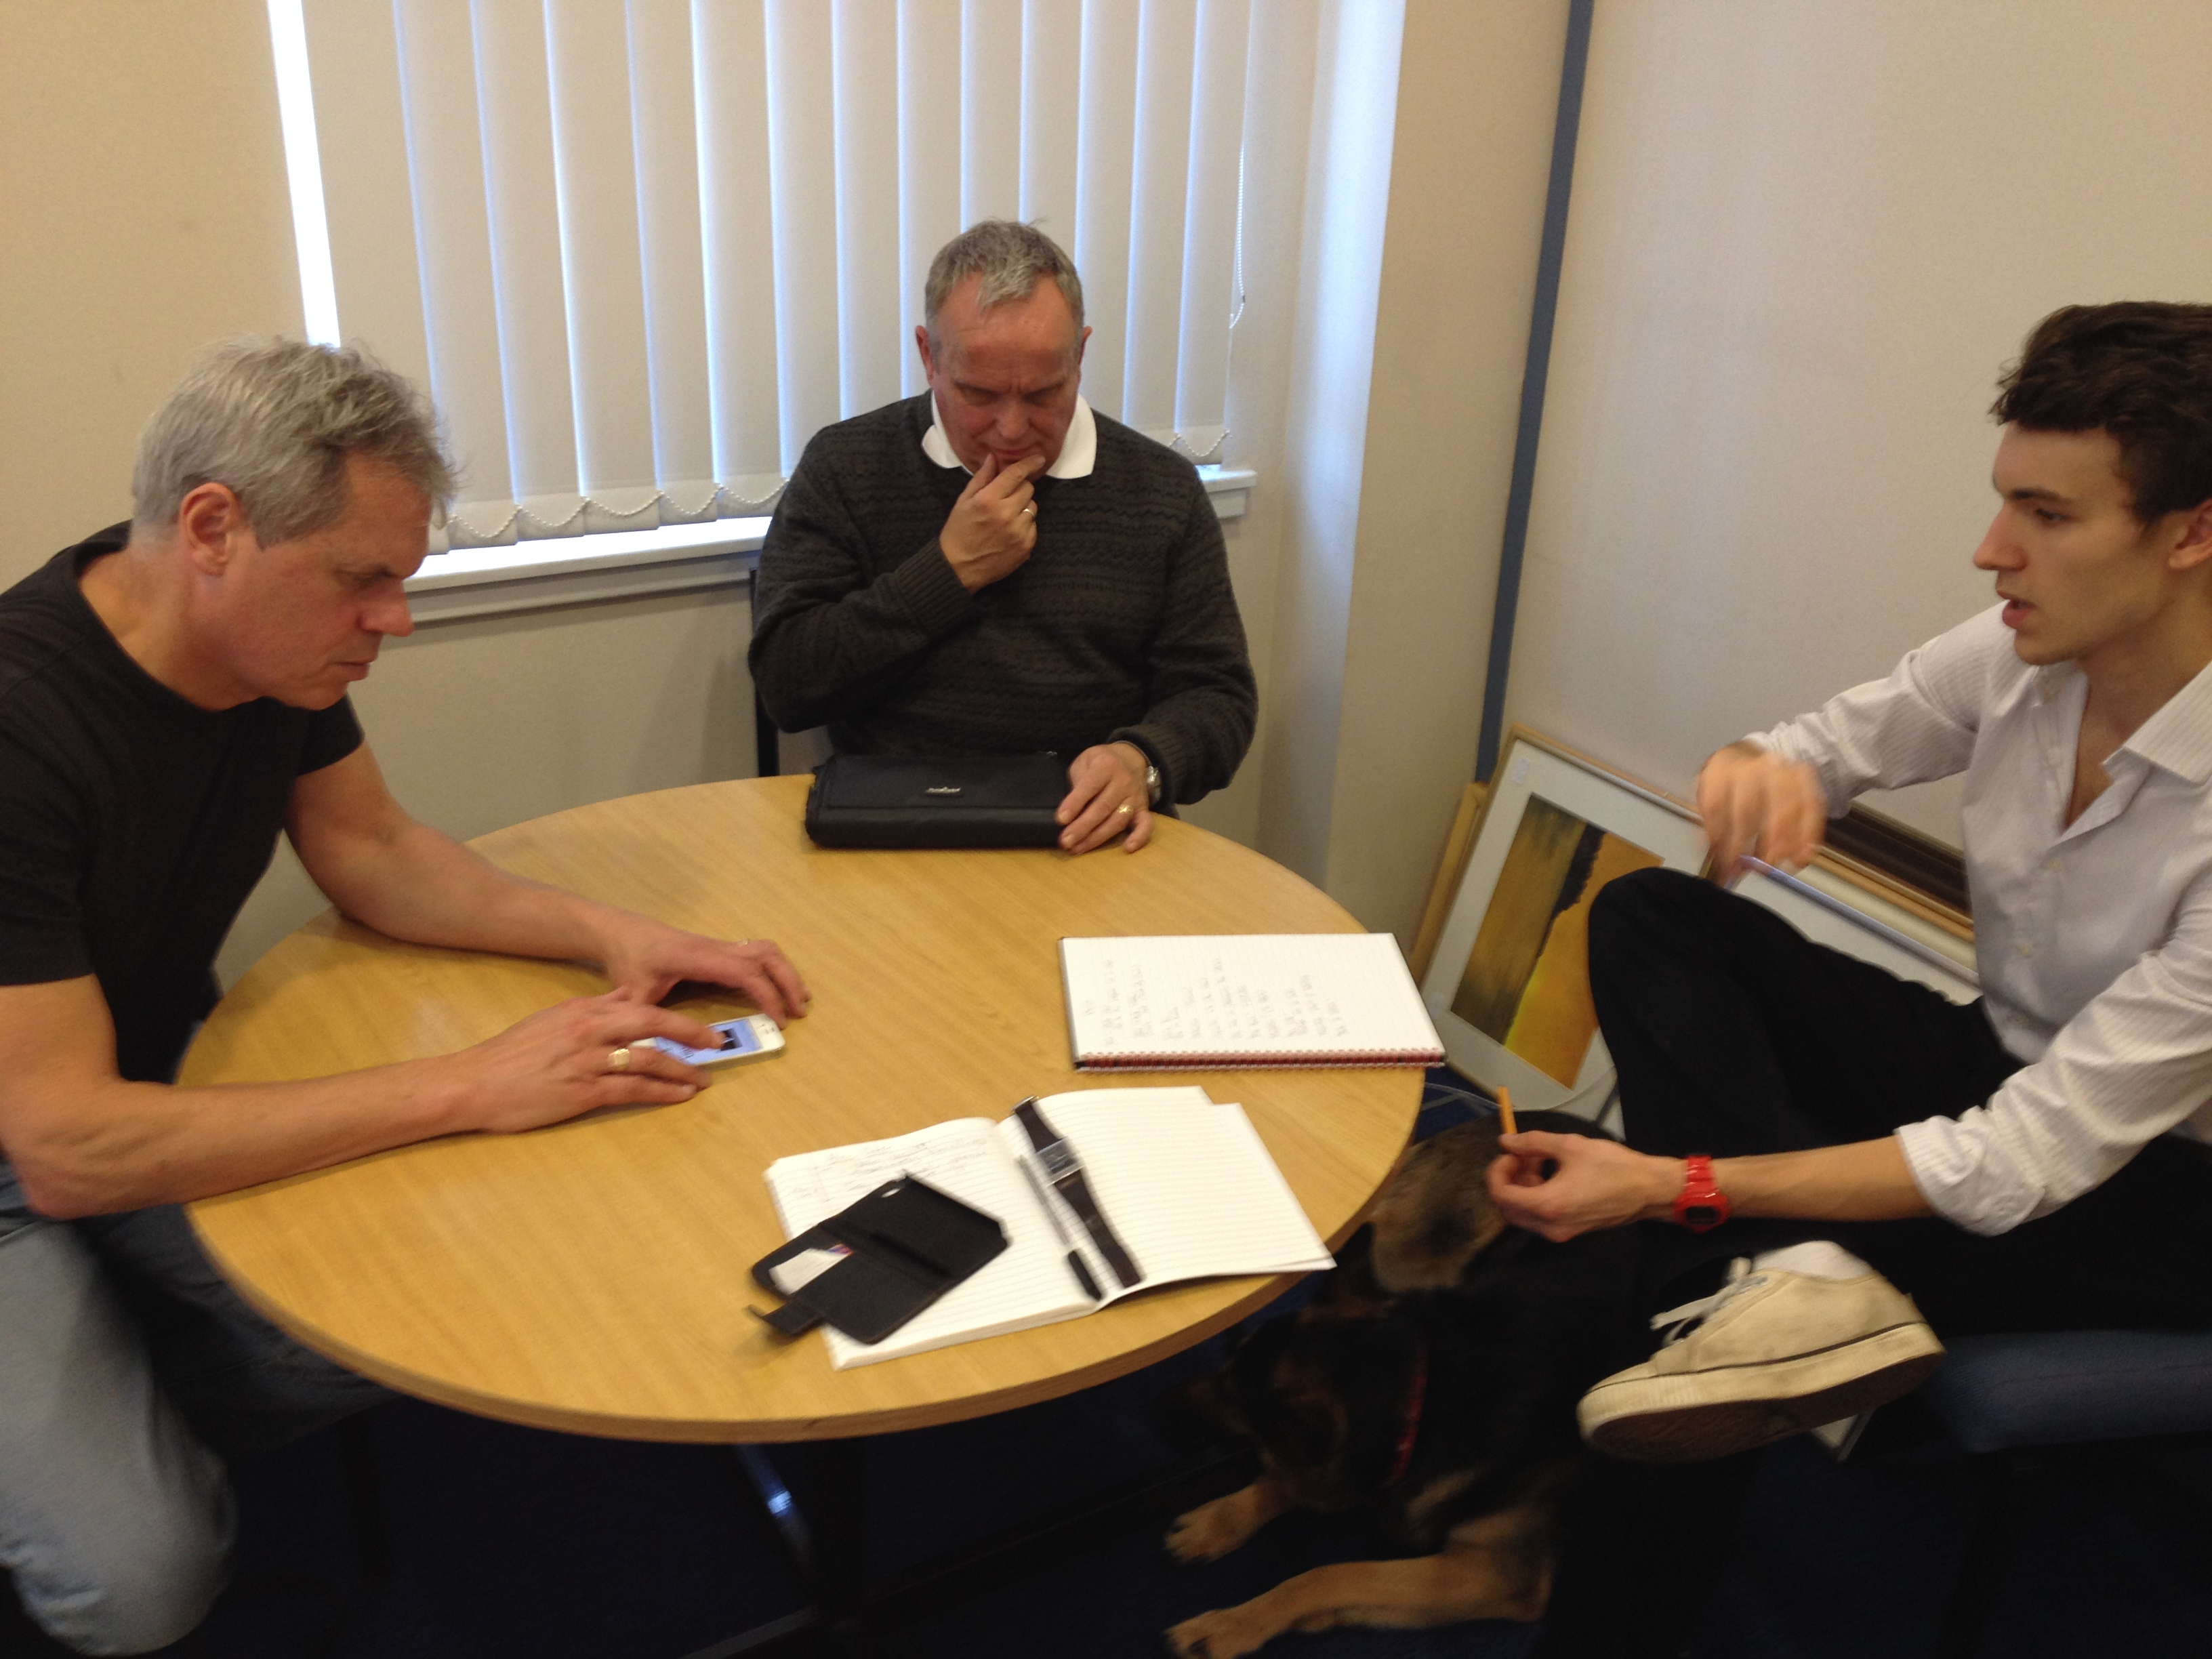
\includegraphics[width=\textwidth]{meeting}
        \caption{Two blind users from the RNIB Mobile User Group trying the Talking Buses app for the first time, 9th October 2013}
    \end{minipage}
    \hspace{0.5cm}
    \begin{minipage}[b]{0.5\linewidth}
        \centering
        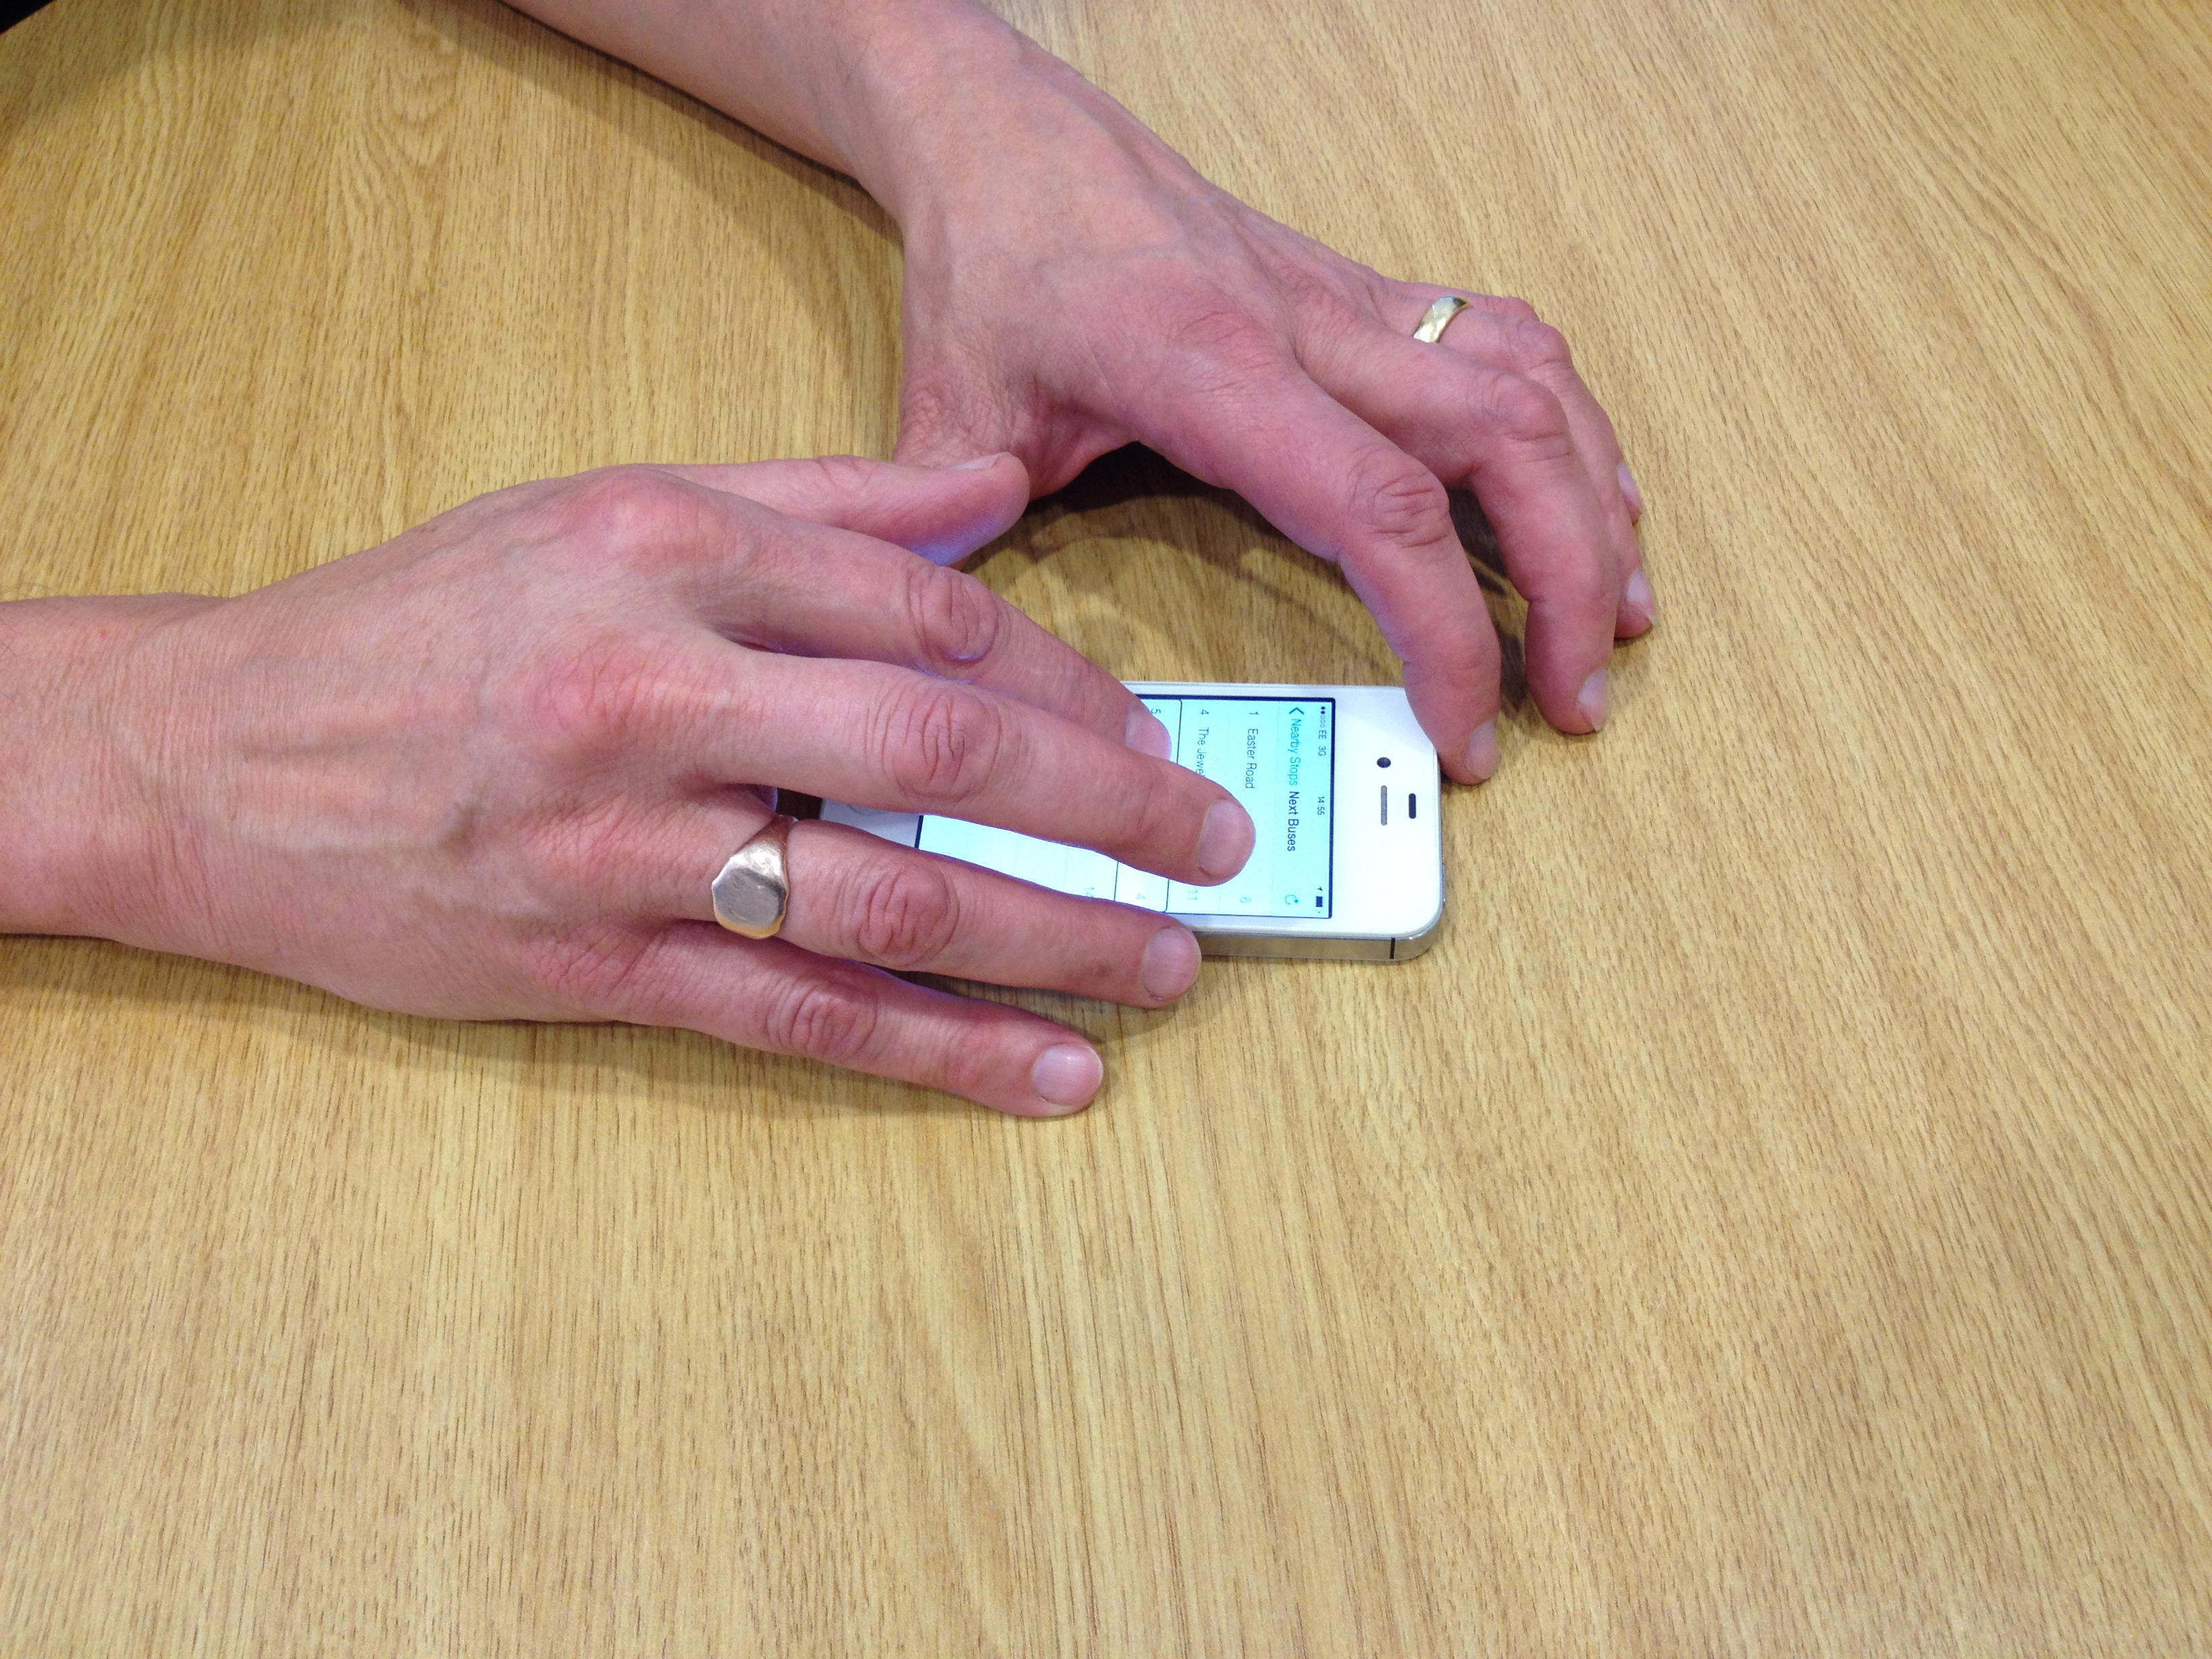
\includegraphics[width=\textwidth]{peter}
        \caption{A blind user tests the use of VoiceOver in the Talking Buses app while finding nearby bus stops}
    \end{minipage}
\end{figure}

\subsubsection{Feature Request: Favourite Bus Stops}
As mentioned above, both members who tested the prototype recognised the benefit of allowing users to store frequently used bus stops, as well as assigning them a self-chosen name (for example, "Home").

In order to add the functionality without disturbing the intuitive user interface, consideration had to be given to how the functionality would be accessed by the users. It was decided that a UITabBarController would be added to the root of the app. This had the effect of adding two tabs to the bottom of the user interface of all screens in the app.

The first tab is labelled "Nearby Stops", and when selected loads a view which presents bus stops nearby the user (as per the original interaction design of the app). The second tab is labelled "Favourite Stops", and displays the list of stops the user has added as favourite bus stops. When the app loads, the first tab is selected by default, and so the user is presented with a list of nearby bus stops (as before).

Additionally, it was decided that selecting a favourite bus stop would have the same result as selecting a nearby bus stop (presenting departures from the bus stop). This means that the user interface remains consistent across all the functionality offered.

To add a bus stop, the user first selects it from the list of nearby bus stops, loading the screen displaying departures from the stop. It was decided that a button would be added to the navigation bar at the top of the screen, which would trigger the process of adding the selected bus stop to the list of favourites.

When the user presses this button, an alert view appears. This alert view asks the user to enter a name for the new favourite bus stop, and provides a text input field and buttons for cancelling and submitting the action. The user moves the VoiceOver cursor to this text input, and either types or dictates a name for the bus stop. Once this is done, the user selects the confirmation button, and the bus stop is added to the list of favourites.

The same solution is used to store favourite bus stops as is used to store regular bus stops, but the objects written to the property list have an extra field: the user-defined name for the bus stop.

When the second tab is selected by the user, this list of favourite bus stops is loaded and displayed to the user. The VoiceOver description for each item in this list is of the same format as that given for nearby bus stops, providing a consistent experience across various functionality in the app. 

\begin{figure}[h!]
  \centering
    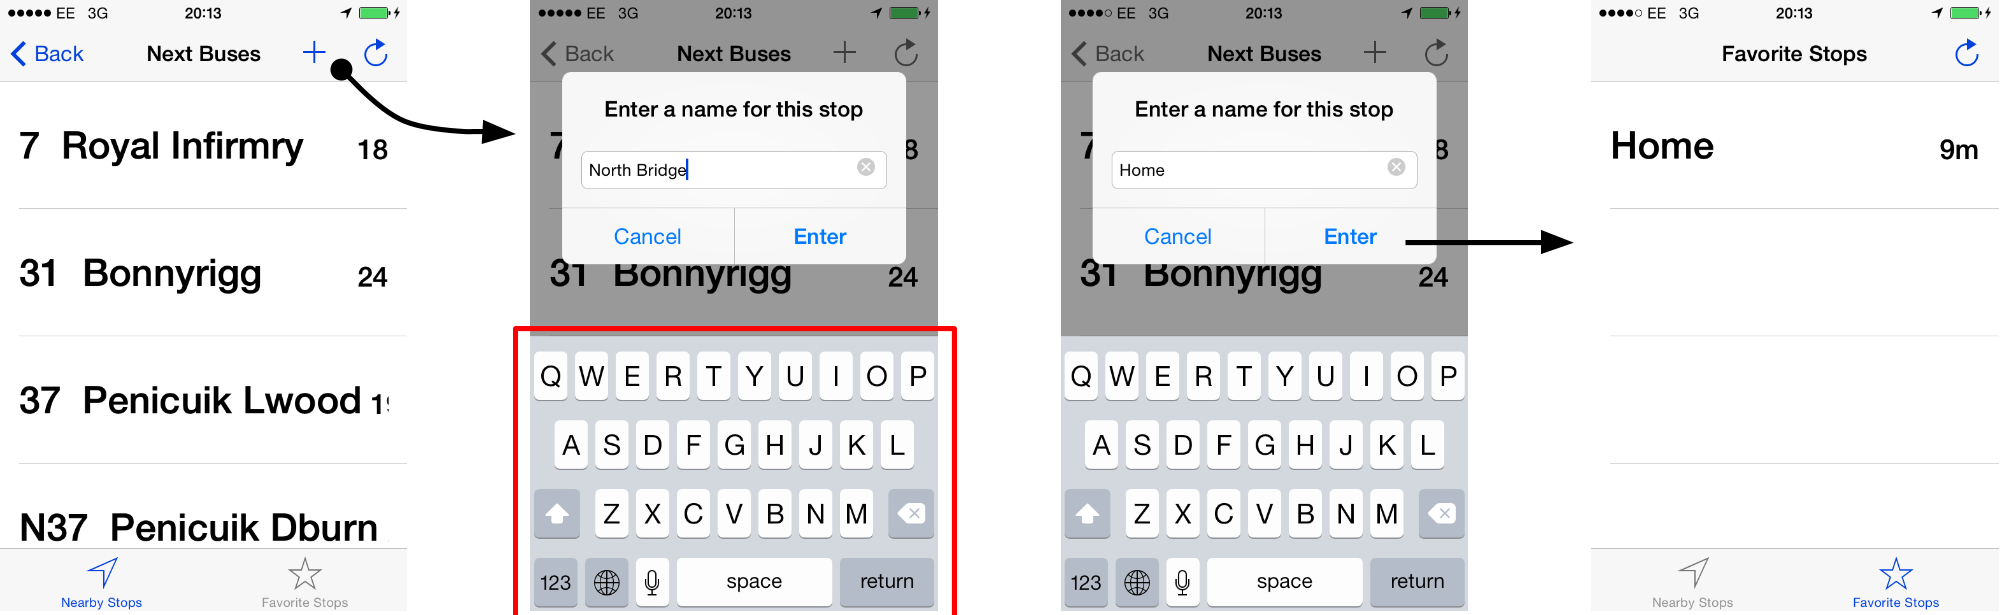
\includegraphics[width=\textwidth]{favFlow}
    \caption{A diagram showing the interaction flow for adding a bus stop as a favourite}
\end{figure}

\subsubsection{Higher Quality Bus Stop Information - NaPTAN}
\label{sec:naptanImp}
Both of the test users from the Mobile User Group agreed that it would be beneficial to include the street names bus stops were located on. This would help to allow blind and partially-sighted users to gain a better understanding of the area surrounding each bus stop.

Another similar issue raised was the generally low quality of bus stop names in the MyBusTracker API. As discussed earlier (Section \ref{sec:myBusTrackerLimitations}), bus stop names are shortened or truncated to eleven characters. This can make the data unsuitable to pass to VoiceOver for dictation, as the results will be unpredictable and potentially confusing to the user. Additionally, the bus stop names often conflict with those printed on the signs at bus stops, which can be confusing for the user.

For these reasons, it was decided that a second source of bus service information would be included in the Talking Buses system.  The NaPTAN database is "a UK nationwide system for uniquely identifying all the points of access to public transport in the UK".

Each bus stop in the MyBusTracker API has an 8-digit bus stop identifier, which is also used by the NaPTAN database. This means that it is possible to augment the information in the MyBusTracker database with higher-quality bus stop names from the NaPTAN database (for which there appears to be no inconvenient upper-limit on length, and which seem to correlate with the printed bus stop names).

Additionally, the NaPTAN database contains street name information for each bus stop in the database. By adding these street names to the documents representing bus stops in the Talking Buses database, the app is able to provide the user with this information when it is useful.

In order to take advantage of the new data, the VoiceOver description for list items representing bus stops was updated to include the street name. This, combined with a higher-quality version of the bus stop name, increased the ability of the app to provide navigation-assistance to blind and partially-sighted users.

The benefits of this are illustrated in Figure \ref{fig:busStopNames}, where we see agreement that the information provided by the Talking Buses app matches that provided in the real world, whereas the information provided by the Lothian Buses app does not.

\begin{figure}[h!]
  \centering
    \fbox{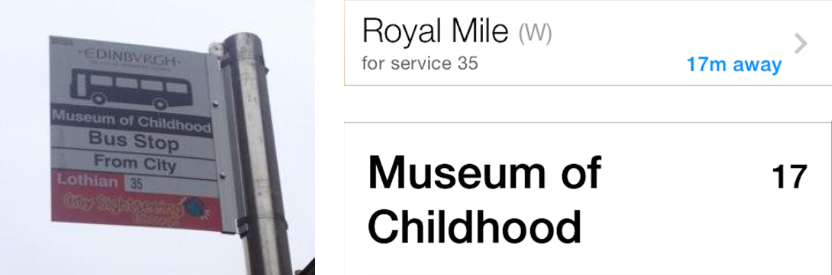
\includegraphics[width=\textwidth]{busStopNames}}
    \caption{Reducing disagreement between the "real" and "virtual" worlds: Use of the NaPTAN database means that the Talking Buses app (bottom-right) provides bus stop names which match those printed on the sign (left) where the Lothian Buses official app (top-right) does not.}
    \label{fig:busStopNames}
\end{figure}

\subsection{Second Iteration}

After the changes described above were implemented, a second meeting was arranged with the RNIB Mobile User Group, in order to receive further feedback and additional suggestions for features This meeting, conducted on November 6th, was well attended, with seven members of the mobile user group in attendance. Of these seven members, five were blind, and two were partially-sighted. Of the two partially-sighted group members, one used VoiceOver to explore the user interface, and the other used a combination of VoiceOver and Zoom, depending on the app used.

At this meeting, the updated version of the Talking Buses app was installed on the iPhone devices of each group member. This provided a fantastic opportunity for feedback, and also allowed for a greater variety of devices for testing than were previously available, as several members of the Mobile User Group owned iPhone 5S devices, released only two months prior. 

Feedback received included the following:
\begin{easylist}[itemize]
& Many users gave positive feedback on the addition of the functionality for adding favourite bus stops, and the restructuring of the user interface to accommodate the change.
& Feedback on the addition of street names to bus stop descriptions was also positive. Users were specifically asked about the resulting length of the description, and agreed that it was still a concise representation of the necessary information.
& One test user requested a new feature be added to the app, allowing users to search for bus stops by name. It was reasoned that this would improve further the planning functionality of the app (after the addition of the favourite bus stops functionality).
& Several users commented on an unfortunate limitation of the app's reliance on occasionally unreliable GPS data from the iPhone. Specifically, they noted that even while stationary, distances given for nearby bus stops had a tendency to fluctuate.
& Several users suggested that arrival times for bus services at a bus stop be grouped together by their service mnemonic to reduce the number of items in the list.
\end{easylist}

\begin{figure}[h]
    \begin{minipage}[b]{0.5\linewidth}
        \centering
        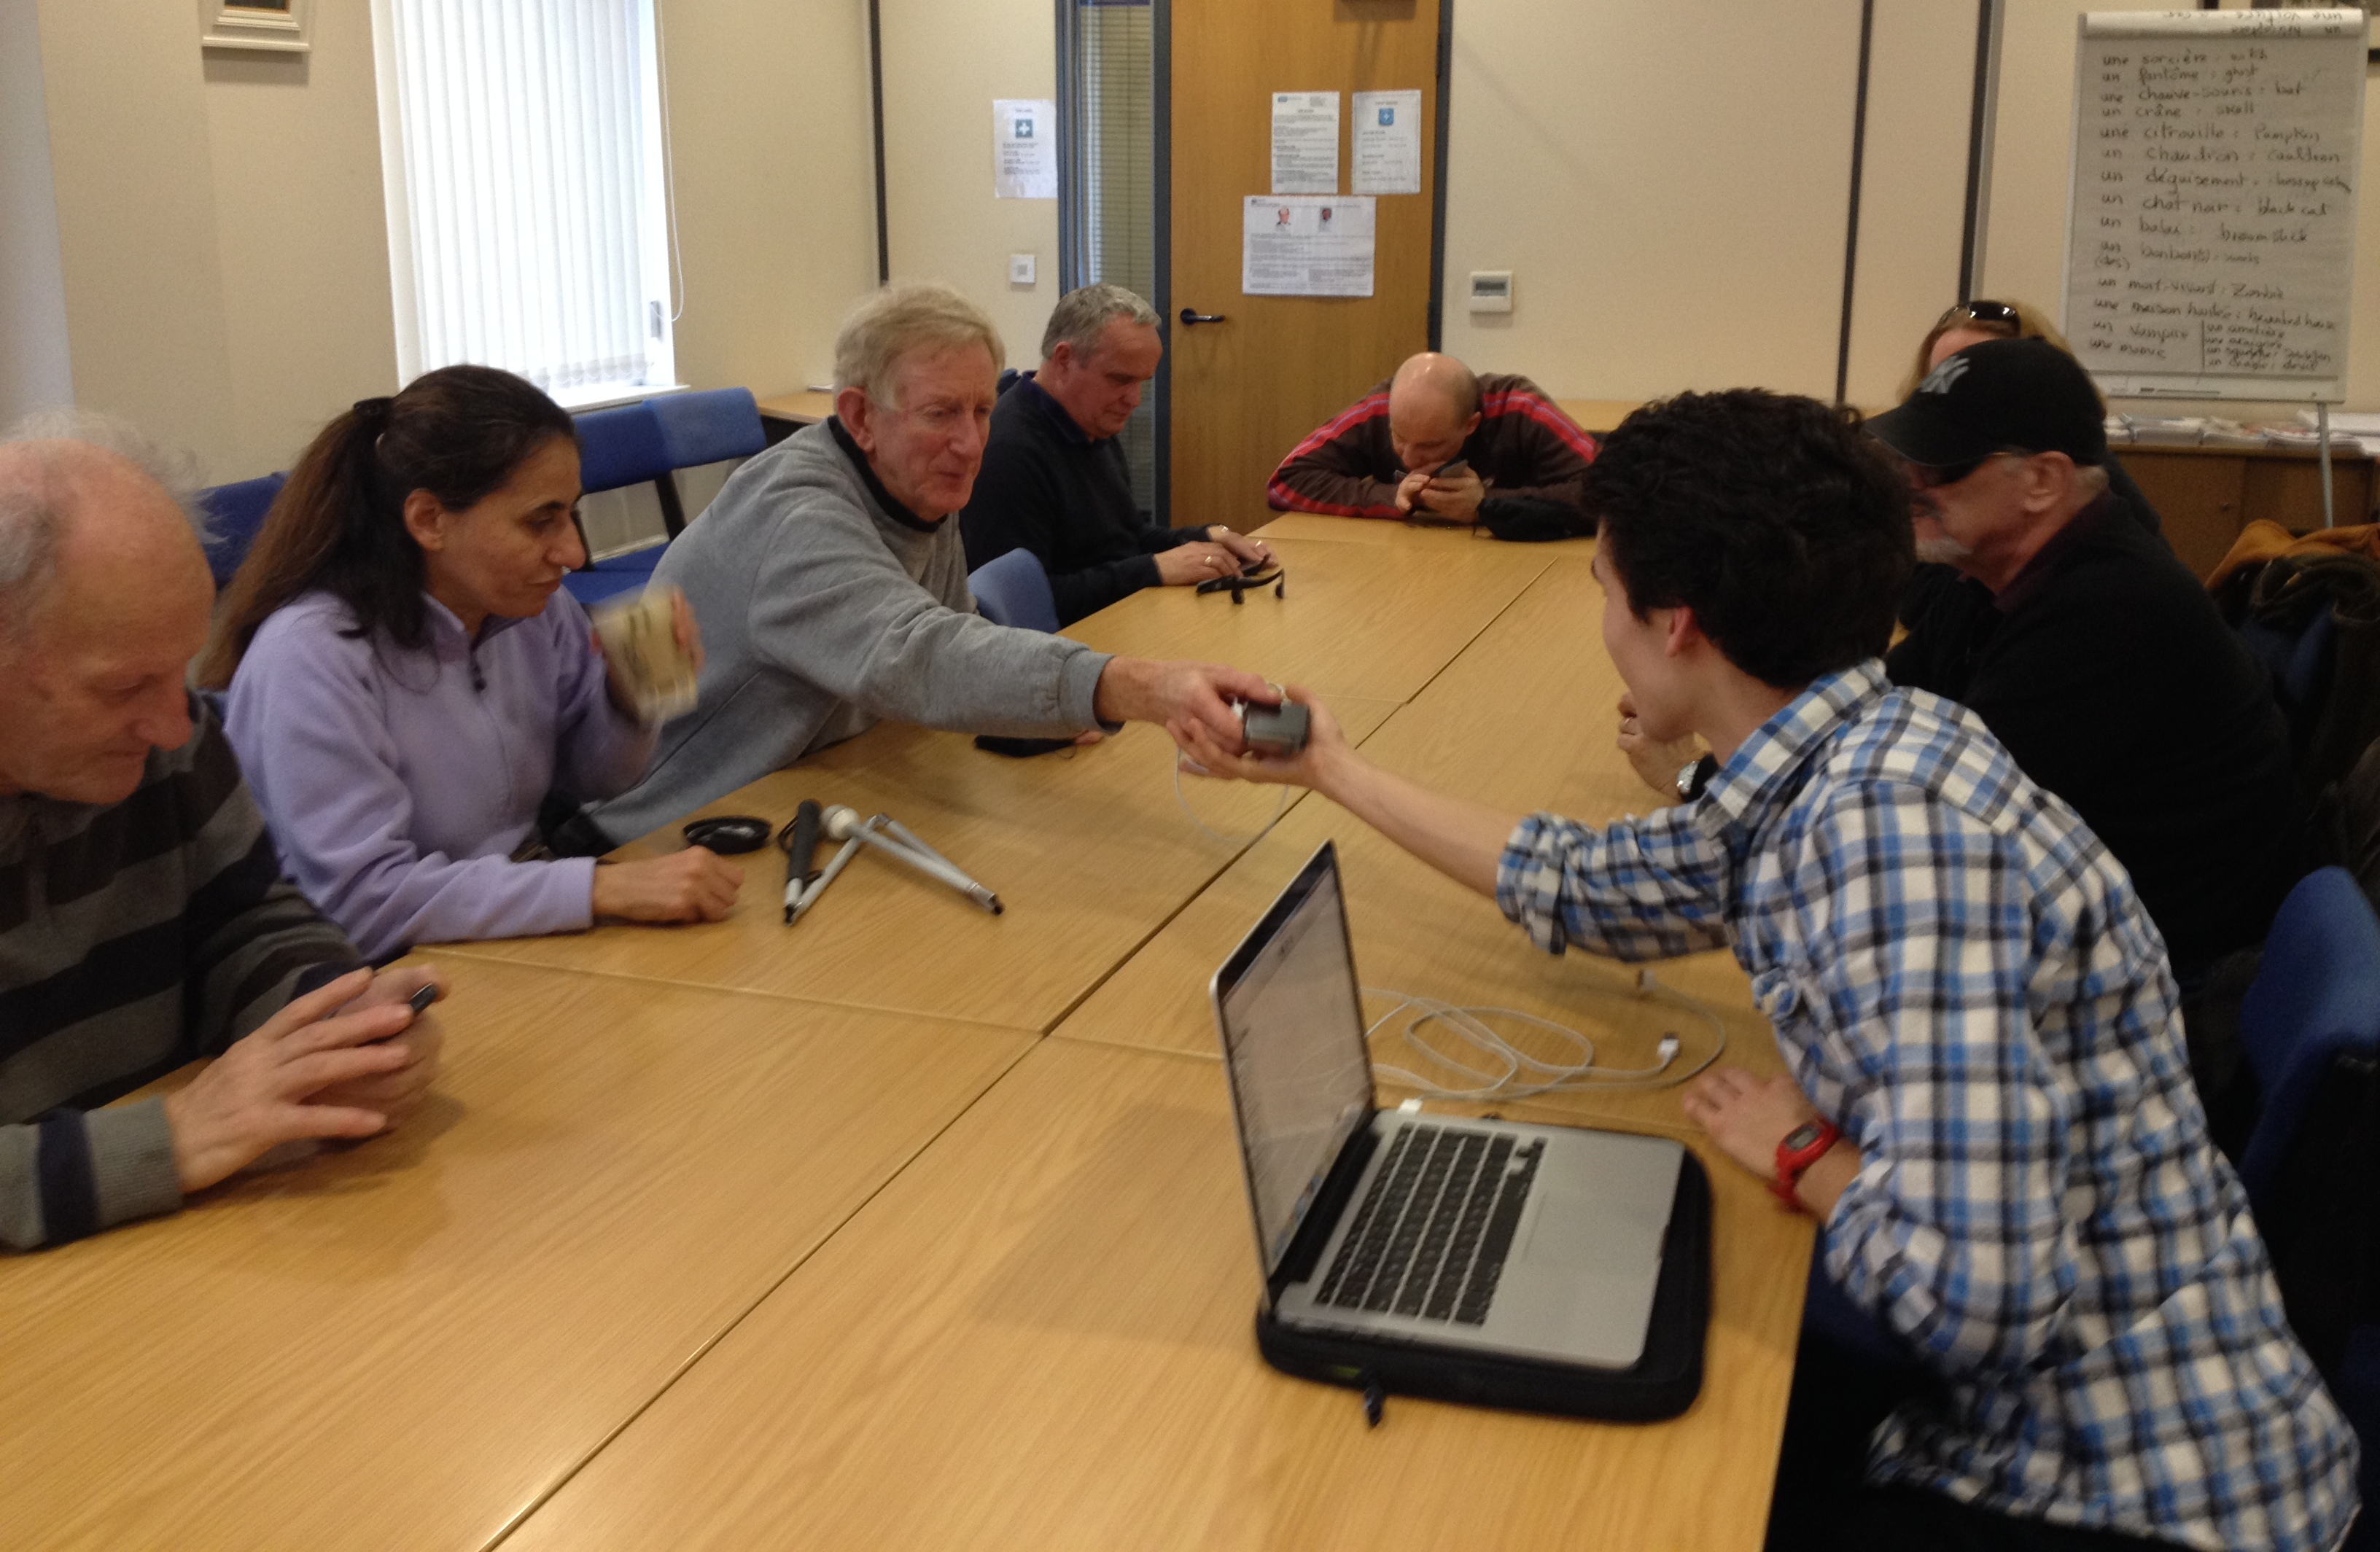
\includegraphics[width=\linewidth]{group}
    \end{minipage}
    \hspace{0.5cm}
    \begin{minipage}[b]{0.5\linewidth}
        \centering
        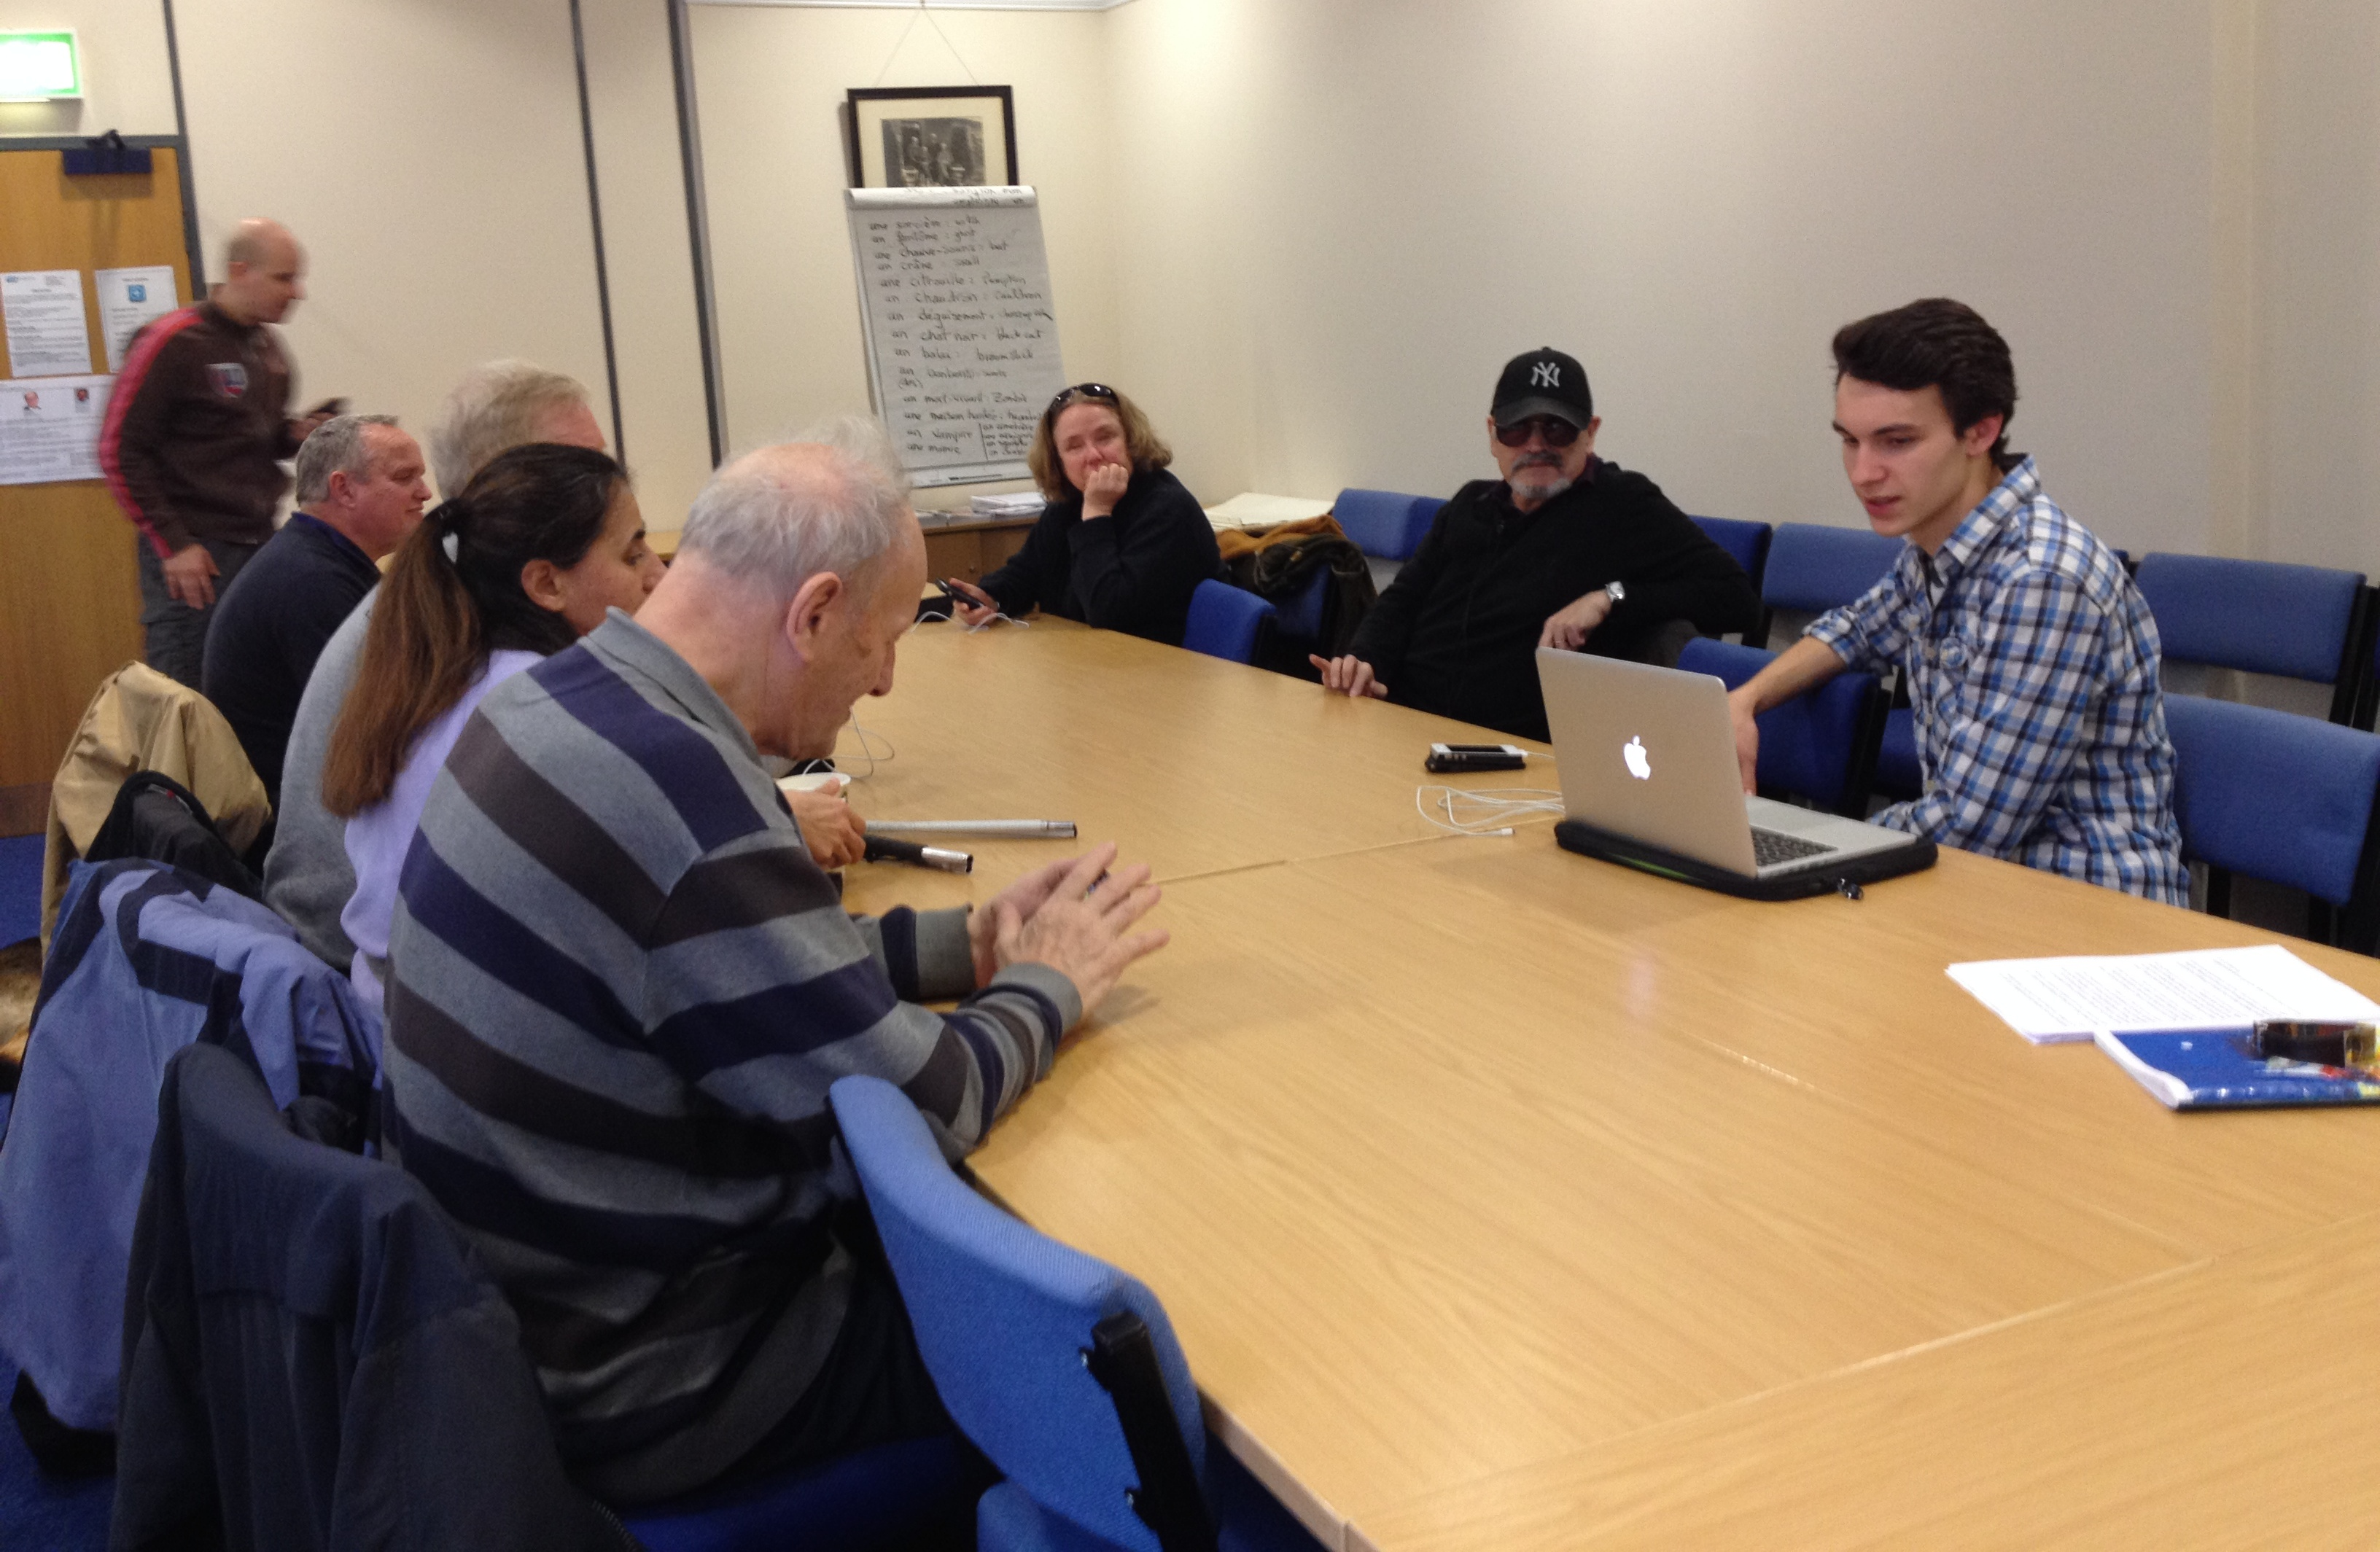
\includegraphics[width=\linewidth]{group2}
    \end{minipage}
    \caption{Installing the next release of the Talking Buses app on RNIB users' devices}
\end{figure}

\subsubsection{Feature Request: Searching for Bus Stops}
Several of the test users from RNIB's Mobile User Group requested the functionality to search for bus stops by name or street name. This functionality would allow a user to find bus service information for any bus stop in the Talking Buses system, massively increasing the app's utility as a travel planning tool for blind and partially-sighted people.

As was done to accommodate the addition of the favourite bus stop functionality, an additional tab was added at the bottom of the user interface on all screens, titled "Search". Selecting this tab loads a user interface which allows the user to enter a search term (by typing on a keyboard or using iOS's built-in dictation feature), and are provided with a list of matching bus stops.

The searching logic was implemented by creating an NSPrediacte object specifying that at least one of two conditions were met by returned bus stops: that the bus stop's name contains the search query, or that the bus stop's street name does.

Selecting a bus stop from this list produces the same result as selecting a nearby or favourite bus stop, meaning we can continue to provide a consistent user experience despite expanding the functionality of the app. Similarly, the format of VoiceOver descriptions used are the same.

\begin{figure}[h!]
  \centering
    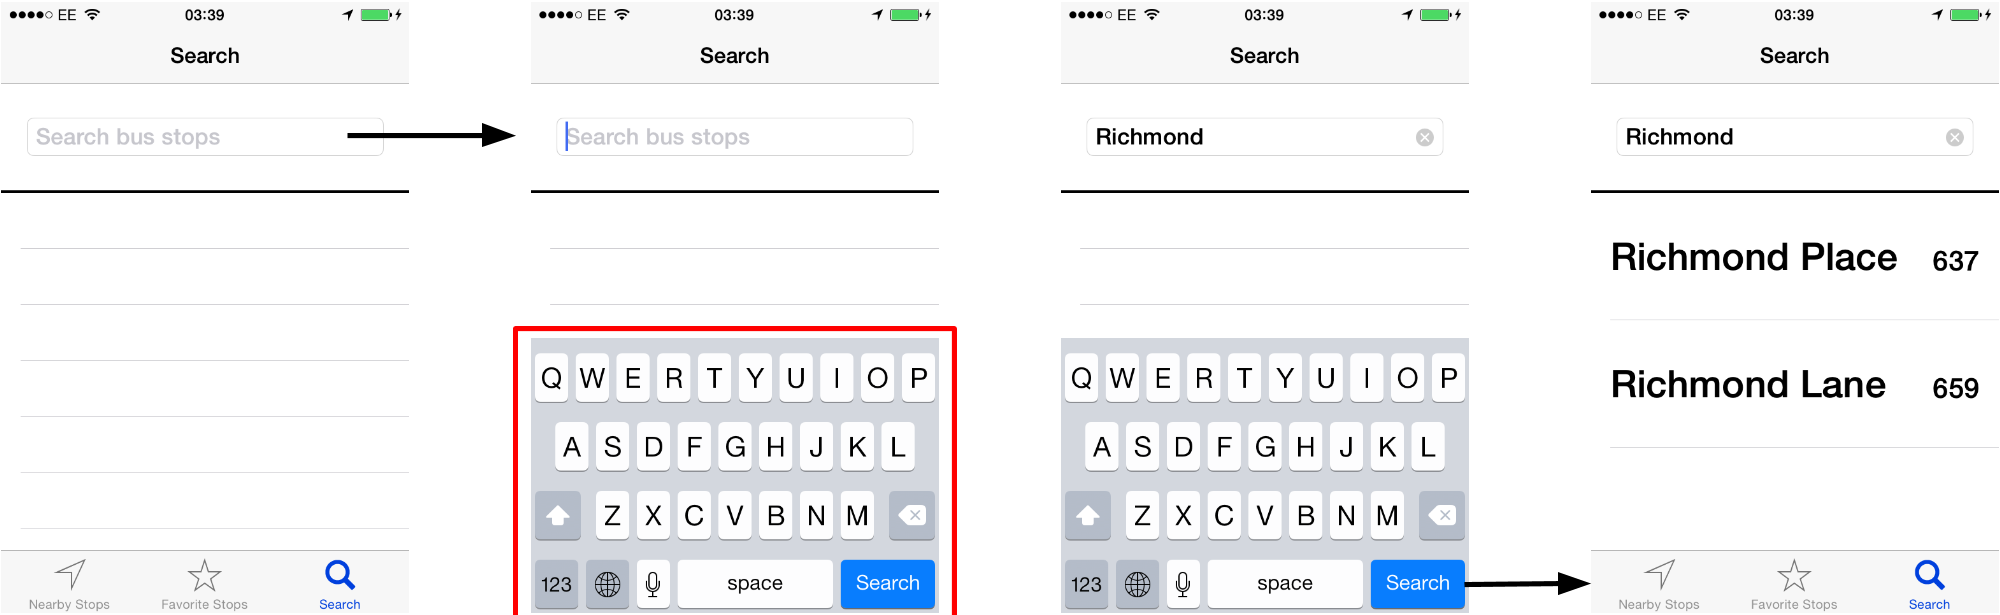
\includegraphics[width=\textwidth]{searchFlow}
    \caption{A diagram showing the interaction flow for searching for bus stops}
\end{figure}

\subsubsection{Grouping of Bus Services When Checking Arrival Times}
Several test users reported that when using the Talking Buses app to check bus service arrival times for a busy bus stop, there was large amount of information in the resulting list. This is due to allocating a row to each individual bus due to arrive for each service.

For this reason, it was decided that the bus arrival times returned by the Talking Buses app would  be grouped by the bus services they belong to. This caused a reduction in the number of items displayed in the list, and an increase in the length of the VoiceOver description of each item (instead of dictating a single arrival time, the app dictates a list of arrival times).

The members of the Mobile User Group agreed that this trade-off was worthwhile, and the change in design was implemented. Users who had the opportunity to evaluate the results of this change (during the cooperative evaluation, described in Section \ref{sec:coopEval}) responded positively.

\subsubsection{GPS Smoothing}
In response to the comments from the test users from the Mobile User Group regarding the accuracy of GPS locations provided by the device, a method of smoothing GPS location data was devised. It was intended that this would provide the app with a more stable fix on the user's location, and therefore allow it to be more accurate in finding bus stops near the user, improving the user's experience.

To accomplish this, when the iOS device receives a location update from the GPS hardware, a simple moving average of the user's latitude and longitude is calculated, respectively. This was implemented by creating a first-in-first-out queue of location updates with a variable length, and then calculating the average latitude and longitude given the number of points in the queue. This average location is then used when calculating the distance to nearby bus stops (instead of the most recently received value, as would be the default behaviour).

The CoreLocation framework provides developers with a variety of information on location updates. Included in this information is an estimation of the instantaneous speed the user is travelling at (expressed in metres per second). This attribute is used to control the size of the list of recent location updates considered in the simple moving average calculations.

\begin{figure}[h!]
  \centering
    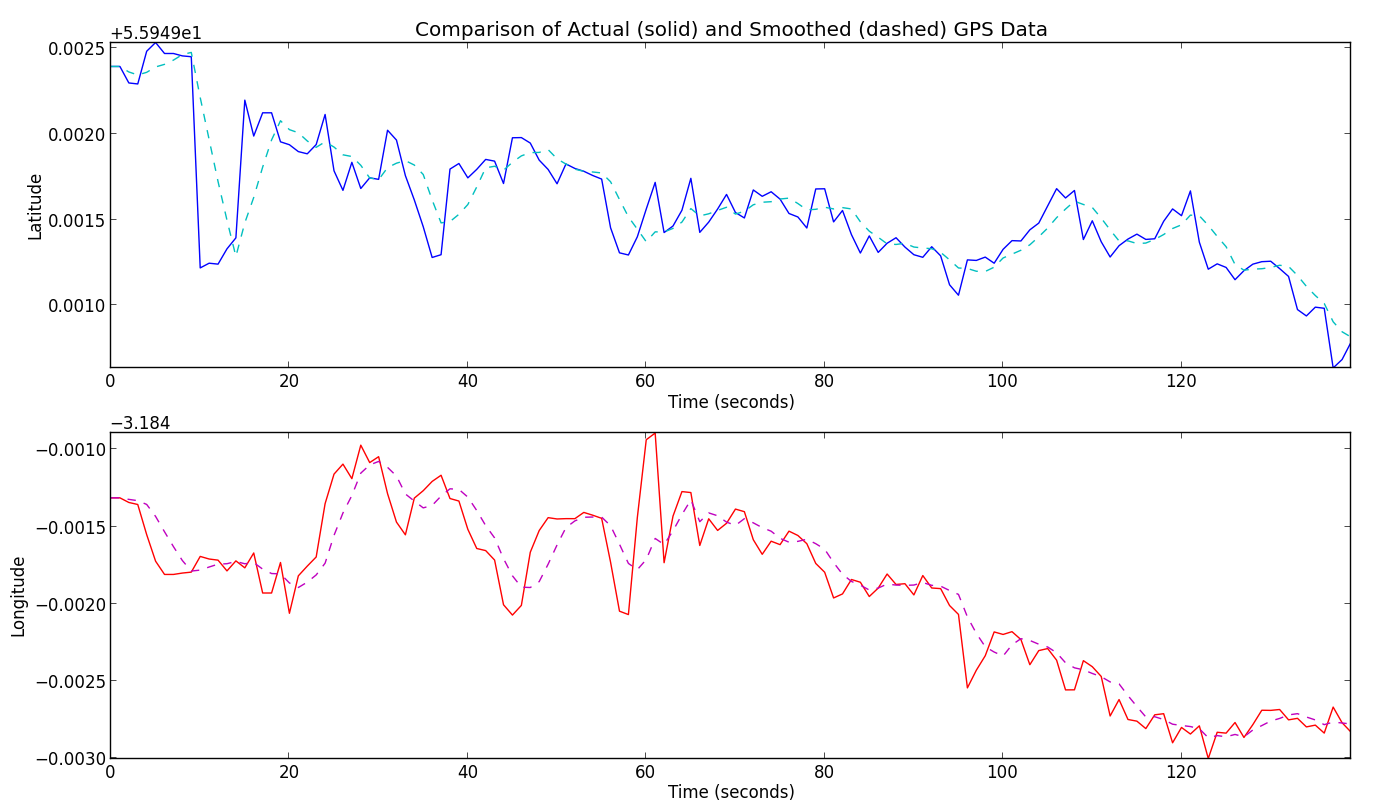
\includegraphics[width=\textwidth]{smoothGraph}
    \caption{Smoothing the GPS data. The solid lines represent the actual latitude and longitude recorded by the device, the dashed lines represent the values used by  the Talking Buses app after smoothing the data.}
\end{figure}

One disadvantage of applying a moving average filter is the inherent delay produced in the GPS data used by the app (as the current location is a combination of the last several). Steps were taken to partially mitigate the effects of this: if the user is deemed to be travelling at over 5 metres per second, the app assumes the user is currently travelling on a bus, and reduces the size of the queue in order to reduce the potential for delay caused by the moving average.

Discussion with the RNIB Mobile User Group confirmed that a slight delay caused by the smoothing was worthwhile given the stability of the resulting location.

\subsection{Summative Evaluation}
\label{sec:summ}
Once the app was deemed to meet the requirements set out for functionality and usability, a summative evaluation took place. Summative evaluations differ from formative evaluations in that they occur at the end of the development phase (instead of providing input to the design phase)

Evaluation of each app was mainly concerned with three areas:
\begin{easylist}[enumerate]
& Functionality - evaluate the extent and accessibility of the functionality offered by the system.
& Experience - gauge the user's experience of the interaction with the system, and the impact the user interface has on the user.
& Problems - locate any specific issues with the system, such as unexpected results, confusion caused to the user, or bugs.
\end{easylist}

In order to produce a meaningful evaluation, the app was compared to the official Lothian Buses app (in its state as of early-2014). Each app was evaluated both by the designer, using a Heuristic Evaluation, and then by the user in a Cooperative Evaluation, as they completed a series of common tasks identified as Use Cases during the design phase (Section \ref{sec:useCases}).

\subsection{Tasks}
\label{sec:evalTasks}
Both apps were evaluated based on the interaction required for the user to complete a series of tasks. These tasks were based on the use cases defined during the design phase (Section \ref{sec:useCases}). Three high-level tasks were identified as common uses of a bus service application, and they are described below.
\begin{easylist}[enumerate]
& Find bus service information from nearby bus stops.
& Find out when the next bus leaves for a particular service from a nearby bus stop.
& Find out the next three bus stops this service calls at, and their estimated times of arrival.
\end{easylist}

These tasks were used as the basis for the heuristic and cooperative evaluations - apps were primarily evaluated on the support they gave users when completing these tasks.

\subsection{Designer Evaluation - Heuristic Evaluation}
A heuristic evaluation is a design evaluation technique used to identify potential issues with usability in the design of a user interface. It is a relatively informal method of evaluation compared to some others, and can be completed without a group of users to test a prototype with.

\subsubsection{Method}
\label{sec:iSimEval}
A heuristic evaluation involves a single individual examining the user interface, evaluating it against a set of recognised usability principles. The principles chosen in the Design subsection (Section \ref{principles}) were used.

A heuristic evaluation was conducted by reviewing the user interface of both the Talking Buses app and the Lothian Buses app, and looking at examples of where each app either conforms to or violates these principles. The VoiceOver descriptions of user-interface elements on the screen were also evaluated in terms of Apple's guidelines for creating suitable VoiceOver attributes.

Lastly, we include a comparison of the performance of the Talking Buses and Lothian Buses official app using the iSimulator (described in Section \ref{sec:iSimDescription}).

\subsubsection{Results}

\textbf{Task 1: Find bus service information from nearby bus stops}
\begin{figure}[h!]
    \begin{minipage}[b]{0.5\linewidth}
        \centering
        \fbox{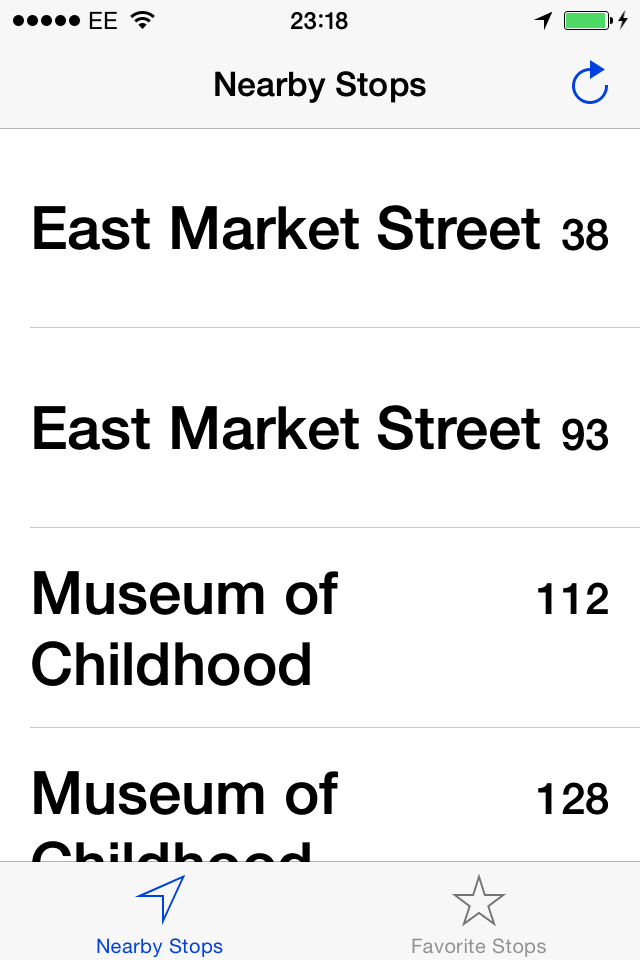
\includegraphics[width=0.7\textwidth]{tb1}}
    \end{minipage}
    \hfill
    \begin{minipage}[b]{0.5\linewidth}
        \centering
        \fbox{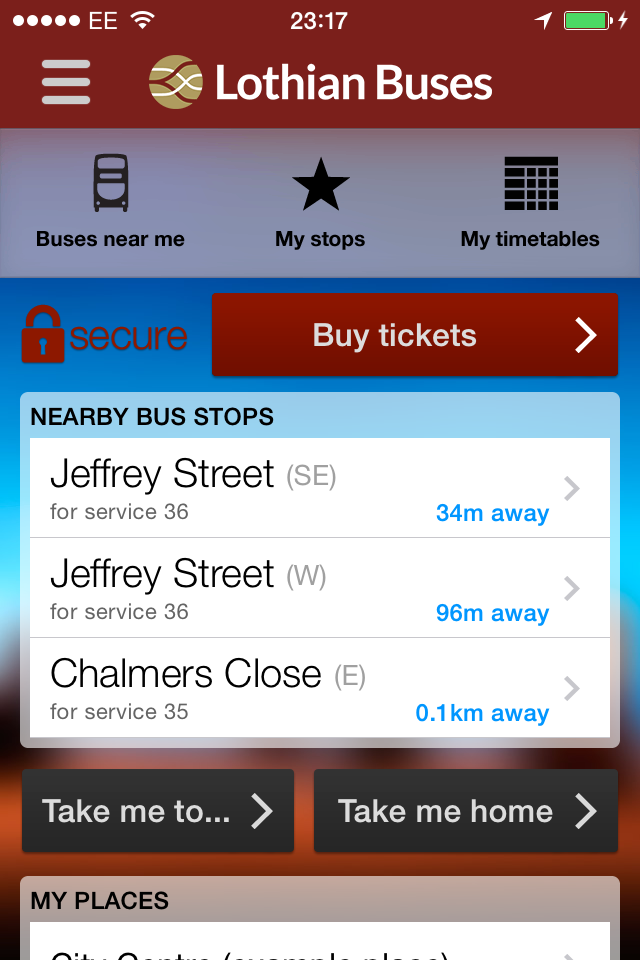
\includegraphics[width=0.7\textwidth]{lb1}}
    \end{minipage}
    \caption{Showing a comparison of the user interfaces designed to allow users to find information on nearby bus stops in the Talking Buses (left) and Lothian Buses (right) apps}
\end{figure}

Several usability issues were identified with the Lothian Buses app for the task of accessing bus service information for nearby bus stops:
\begin{easylist}[itemize]
& A variety of text sizes are used to convey information to the user visually, some of which are too small to be accessible to partially-sighted users.
& The user interface is fairly cluttered (containing 12 accessible elements, compared to the 6 displayed on the Talking Buses app's user interface), which makes VoiceOver interaction more time consuming, and interpretation of the user interface by a partially-sighted user more challenging. The use of a background image could cause colour contrast issues for partially-sighted users.
& The ordering of user interface elements often does not correspond to their importance in terms of the popularity of functionality offered. For example, a VoiceOver user must advance the cursor a total of nine times before they reach information on nearby bus stops.
& Some of the information is not suitable for pronunciation by VoiceOver. For example, bus stop headings are shortened to a single letter ("N" for "North" and so on). This means the VoiceOver for a bus stop becomes: "Jeffrey Street. W. For service...", providing a poor experience for users of VoiceOver.
\end{easylist}

\textbf{Task 2: Find out when the next bus leaves for a particular service from a nearby bus stop}
\begin{figure}[h]
    \begin{minipage}[b]{0.5\linewidth}
        \centering
        \fbox{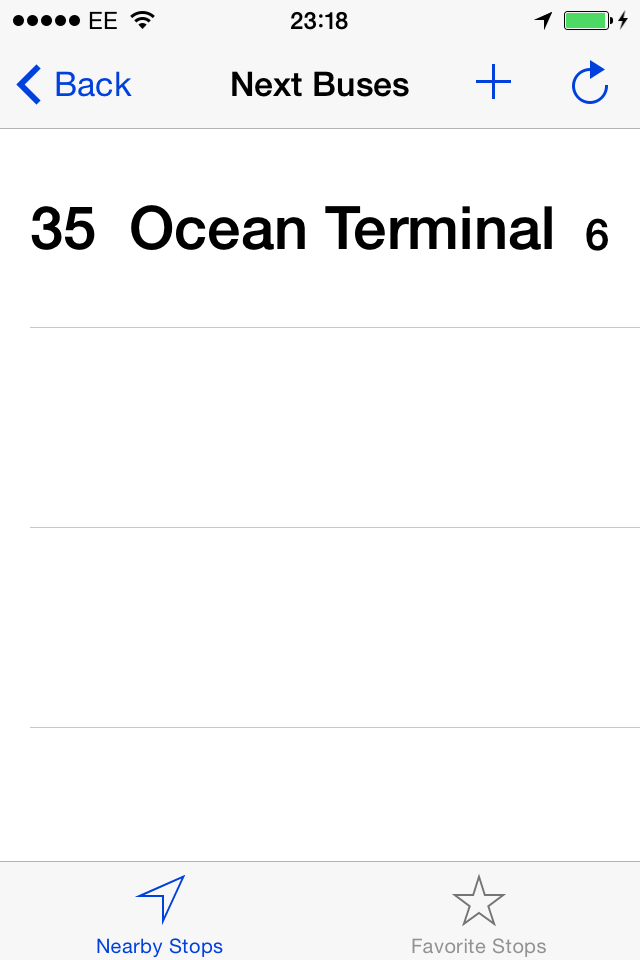
\includegraphics[width=0.7\textwidth]{tb2}}
    \end{minipage}
    \hfill
    \begin{minipage}[b]{0.5\linewidth}
        \centering
        \fbox{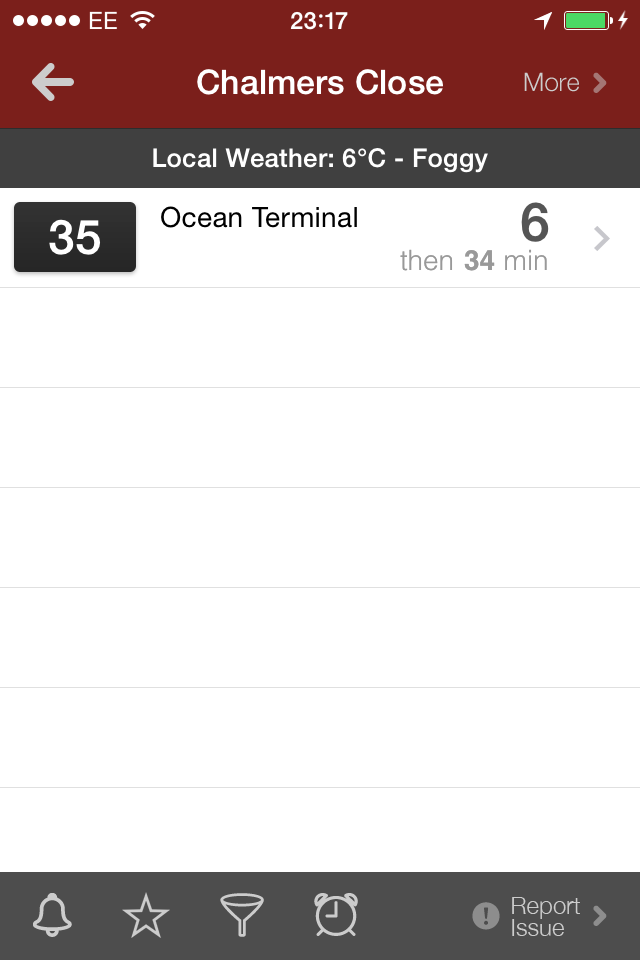
\includegraphics[width=0.7\textwidth]{lb2}}
    \end{minipage}
    \caption{Showing a comparison of the user interfaces designed to allow users to find departure times for a particular bus stop in the Talking Buses (left) and Lothian Buses (right) apps}
\end{figure}

A number of issues were identified with the accessibility of the Lothian Buses app when fetching bus service information for a selected bus stop:
\begin{easylist}[itemize]
& As in the previous user interface, some of the text displayed on the screen has too small a font size to be accessible to partially-sighted users
& The ordering of elements in the user interface again contradicts the value of the information offered by each. Before a VoiceOver user can access information on bus services calling at the stop, they must move the cursor through an element which gives a description of the current weather.
& None of the user interface elements have their hint accessibility attribute set, making it challenging for a VoiceOver user to predict the actions of interacting with them.
& Many of the user interface elements include the type of the element in their VoiceOver accessibility label attribute. This can make VoiceOver descriptions for certain elements confusing. For example, the button located at the bottom of the interface which adds the bus stop to the user's favourites produces the VoiceOver description: "Icon Add Favourite, Button". 
\end{easylist}

\textbf{Task 3: Find out the next three bus stops this service calls at, and their estimated times of arrival}
\begin{figure}[h]
    \begin{minipage}[b]{0.5\linewidth}
        \centering
        \fbox{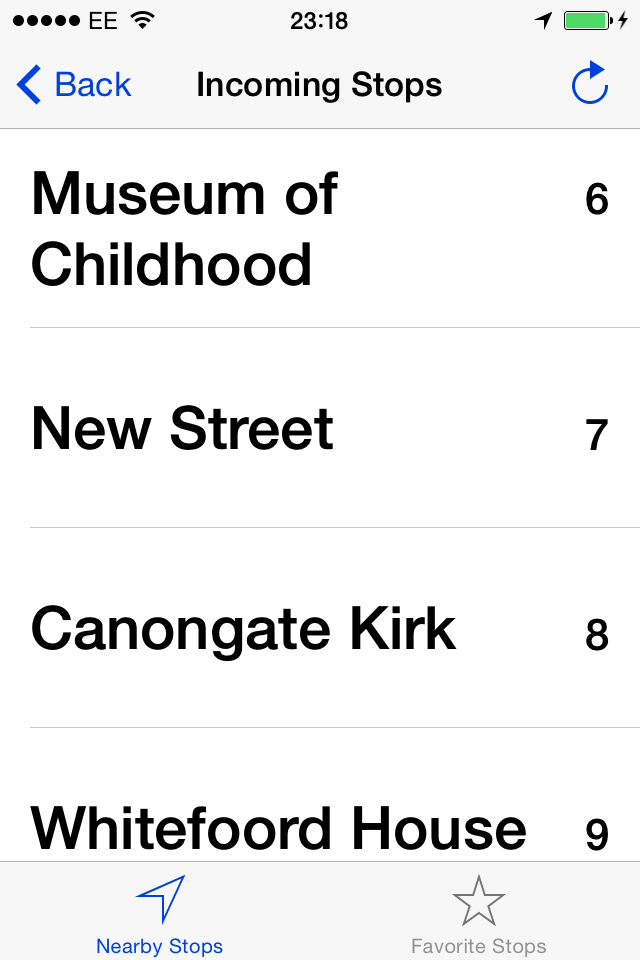
\includegraphics[width=0.7\textwidth]{tb3}}
    \end{minipage}
    \hfill
    \begin{minipage}[b]{0.5\linewidth}
        \centering
        \fbox{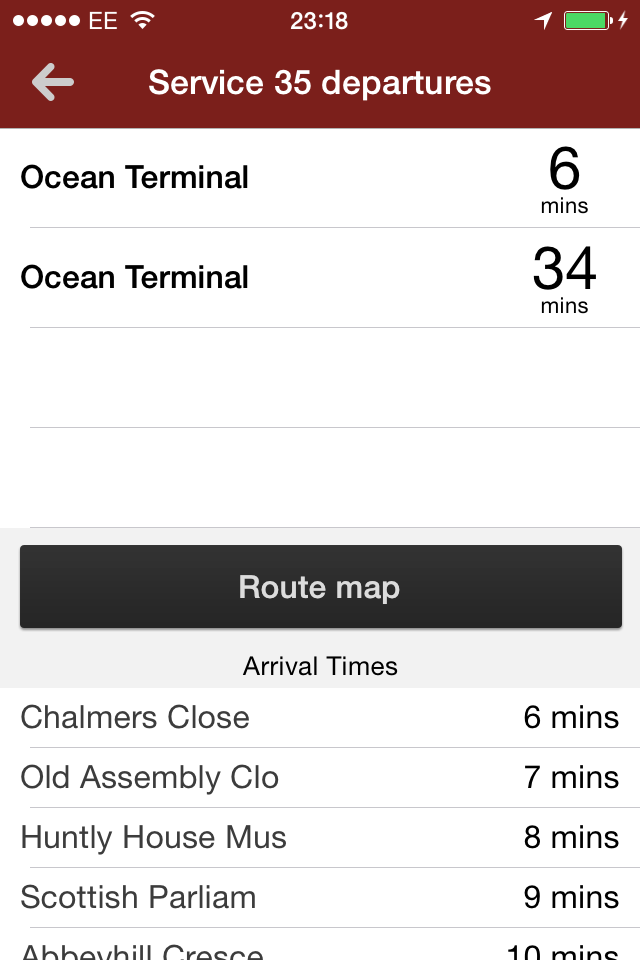
\includegraphics[width=0.7\textwidth]{lb3}}
    \end{minipage}
    \caption{Showing a comparison of the user interfaces designed to allow users to find information on incoming bus stops in the Talking Buses (left) and Lothian Buses (right) apps}
\end{figure}

Several issues were identified with the Lothian Buses app when finding information on bus stops a chosen bus service calls at:
\begin{easylist}[itemize]
& Some of the user interface elements are too small to be easily accessed using VoiceOver. For example, each item in the list of arrival times provided at the bottom of the user interface is only allocated 30 pixels vertically (compared to 100 pixels in the Talking Buses app)
& Much of the text used in the user interface is too small to be accessible for partially-sighted users.
\end{easylist}

\begin{figure}[hbtp]
    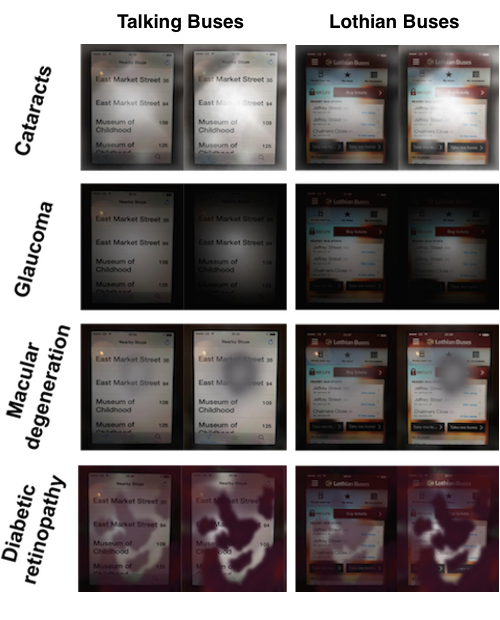
\includegraphics{iSim_all}
    \caption{iSimulator images for the Talking Buses (left) and Lothian Buses (right) apps, simulating the effects of visual impairments in varying degrees}
    \label{fig:iSim_all}
\end{figure}

\subsubsection{Summary}

The most significant issue identified with the Lothian Buses official app for blind and partially-sighted users was that the implementation of VoiceOver has not been in accordance with the guidelines provided by Apple.

Many of the user-interface elements examined during the evaluation were non-standard meaning that they had been implemented by the developers of the Lothian Buses app as an alternative to customising the default elements provided on iOS. When using non-standard user-interface elements, it is the responsibility of the developer to provide the appropriate VoiceOver attributes (label, value, traits, and a hint).

Many of the non-standard elements in the Lothian Buses app failed to provide a hint attribute (for example, the "Main Menu" button at the top left of the home screen). This means that a VoiceOver user is unable to reliably predict the results of interacting with the element. This makes the app more challenging to use successfully, especially for first-time users.

Additionally, several elements which provided the required accessibility attributes did so using values which were not suitable for dictation by VoiceOver (for example, providing "W" instead of "West" when providing descriptions of nearby bus stops). This can make information supplied by the app to a VoiceOver user challenging to understand, potentially making use of the app frustrating.

In contrast, care has been taken in the Talking Buses app to provide all of the required VoiceOver attributes for user-interface elements for any non-standard elements, and default attributes of standard user-interface elements has been customised where appropriate (for example, the hint supplied for the "Refresh" button located on many screens in the app). Additionally, efforts were made where possible to ensure that information passed to VoiceOver for dictation was be pronounced correctly (for example, supplying a complete word for descriptions of bus stop headings, e.g. "West",  as opposed to a single character, e.g. "W")

The other main issues identified were largely concerned with the visual design of the Lothian Buses app. In several places, text displayed to the user was too small to be accessible to partially-sighted users (such as the labels of bus stop names a given bus service was due to arrive at). The home screen uses an image for the background, decreasing the contrast between some of the text on the screen and the background.

The effects of these design decisions are illustrated in Figure \ref{fig:iSim_all} , for the Talking Buses app and Lothian Buses official app. In several of these images, the Talking Buses screenshot is legible where the equivalent Lothian Buses screenshot is not, largely due to the use of larger, bolder fonts and use of fewer colours. Due to the Layout of the Lothian Buses app, there are several cases where entire user-interface elements are obscured, which is not generally the case with the Talking Buses user interface until the image representing the greatest severity (except in the case of Glaucoma, which is particularly detrimental for both apps).

Because the Talking Buses app was specifically designed for blind and partially-sighted users, more consideration has been given to how the visual design will affect the accessibility of the app for these users. Any text displayed is of an appropriate size and font, and the user-interface was designed with simplicity and clarity in mind.

\subsection{User Evaluation - Cooperative Evaluation}
\label{sec:coopEval}
A cooperative evaluation involves the intended user carrying out the task with direct feedback to and from the evaluator of the user interface. The user can ask for help when they are stuck, and are asked questions about their understanding of the system, its commands and responses.

Cooperative evaluations are useful as they create a dialogue between users, designers and evaluators. Given the needs of the intended user, it is intuitively more important to have a thorough understanding of the user's interpretation of the user interface than usual. As our users are not accessing a visual representation of the current state of the system, a greater understanding of how the user is receiving feedback and incorporating it into decisions is arguably required. 

\textbf{User Groups}:

The evaluation was conducted with two groups of users: blind and partially-sighted smartphone users from RNIB's Mobile User Group, and a selection of sighted smartphone users from the university and other sources. The decision to also test with sighted users was motivated by the desire to have testers who would be able to focus on evaluating the app in terms of general performance and functionality.

Six testers participated in the cooperative evaluation. Test users were aged between 20 and 70. Four of the testers were male, the other two were female. Four of the testers were blind or partially-sighted, and two were sighted users (testing purely for performance and functionality). Of the test users, all said that they both owned a smartphone and were comfortable with smartphone technology. The four blind and partially-sighted testers were all familiar with accessibility technologies available on iOS.

Three of the testers used bus services as frequently as several times a day, the remaining three testers used bus services several times a month. Two of the blind users did not use an existing app to aid with bus travel, one of the blind test users and the partially-sighted test user both used the Lothian Buses Official app. Both of the sighted users used the Edinbus app.

\textbf{Video Recording}

In order to gain as much meaningful information as possible during the cooperative evaluation, two cameras were used to record video and audio:
\begin{easylist}[enumerate]
& A \textit{FaceTime} webcam, located above the screen on the evaluator's MacBook Pro. This was used to record the tester's facial expressions as they interacted with the app, allowing for an insight into aspects of tasks with high cognitive demand, or app behaviour which confused or pleased the tester.
& A webcam mounted on a flexible arm connected to a 'cradle' in which the testing device was placed. This allowed for the recording of the device's screen and the tester's interaction with it. This equipment is especially useful when evaluating a VoiceOver app, as it allows the evaluator to see how the tester is using VoiceOver gestures to navigate the user interface, and how the interface of the app is responding to the actions of the user.
\end{easylist}

\begin{figure}[h!]
  \centering
    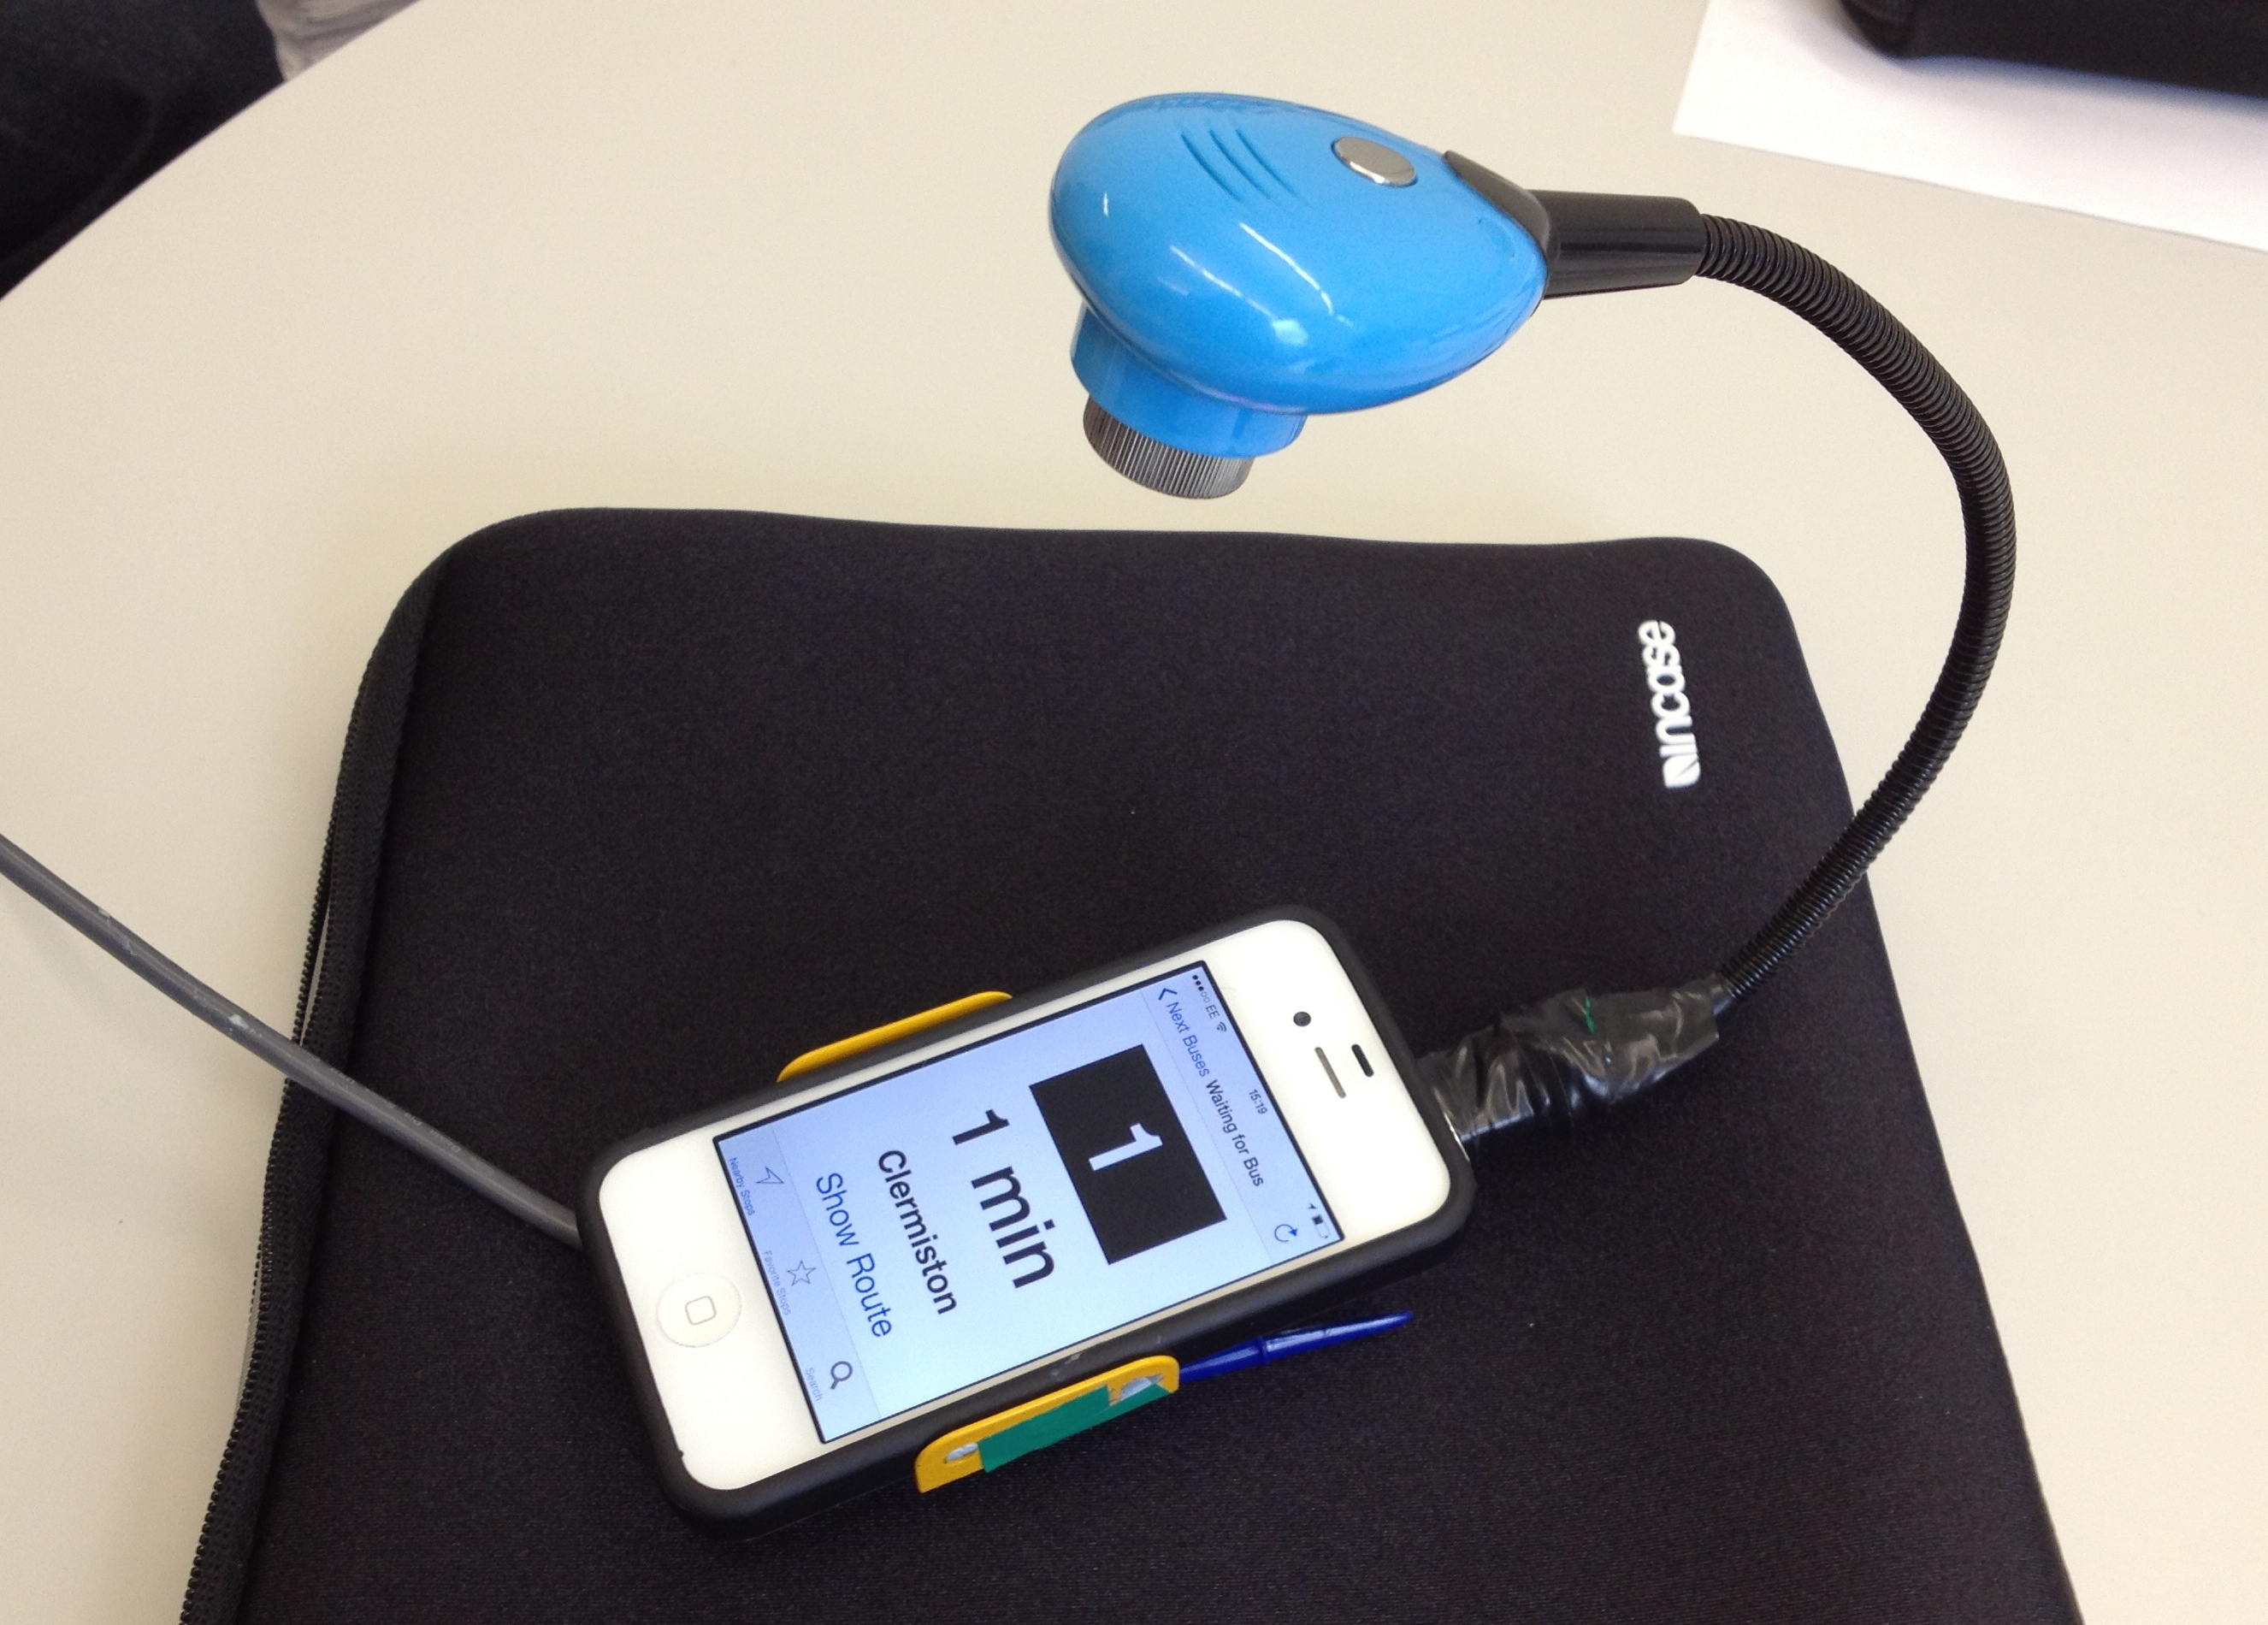
\includegraphics[width=0.5\textwidth]{rig}
    \caption{Video recording equipment designed to record the device's screen and the hands of the user as they interact with the device}
\end{figure}

It was deemed advantageous to combine the two individual video sources to allow for simultaneous playback for transcribing or analysing recordings taken during cooperative evaluations. This was accomplished using a combination of two free pieces of software for Mac OS X:
\begin{easylist}[enumerate]
& \textbf{CamTwist} is a video processing suite capable of applying affects in real time to multiple video streams. CamTwist was use to rotate the video stream from the iPhone-mounted camera 180 degrees (as the camera's actual orientation is incorrect), and place it side-by-side with the stream from the FaceTime camera, combining them into a single video source
& \textbf{QuickTime Broadcaster} is a live video encoding tool developed by Apple, and is used to capture and record the combined video stream from CamTwist to disk.
\end{easylist}

\begin{figure}[h!]
  \centering
    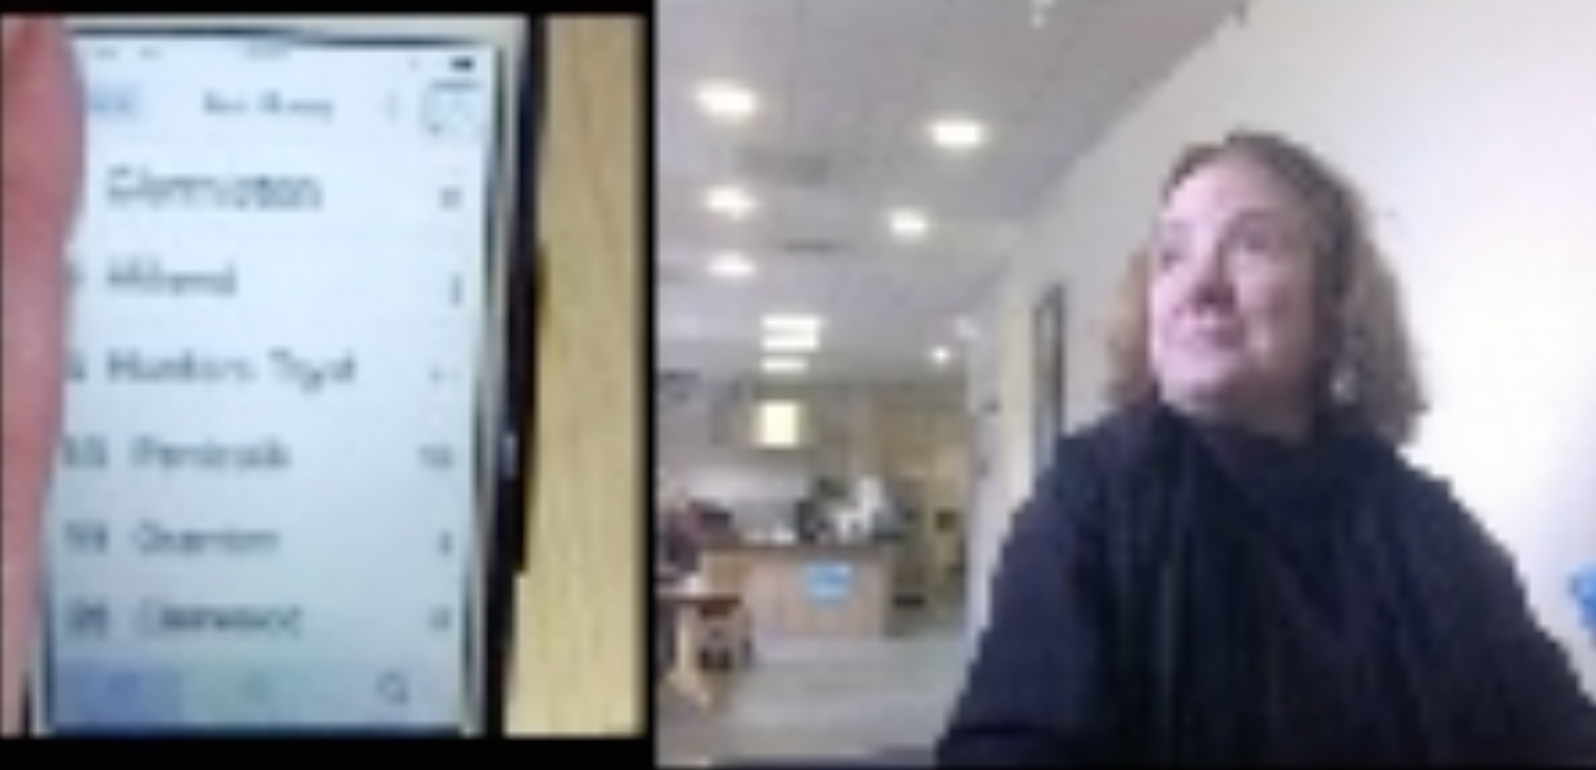
\includegraphics[width=0.7\textwidth]{combined}
    \caption{The two video streams captured during the evaluation, combined using CamTwist}
\end{figure}

\subsubsection{Method}

The evaluation consisted of the following stages:
\begin{easylist}[enumerate]
& A short consent form was dictated, discussed and signed by the tester.
& A pre-evaluation survey was conducted, in order to learn more about each user's level of vision, experience with accessibility technologies, and bus service usage.
& For each app being tested (Talking Buses, and the official Lothian Buses app):
&& A cooperative evaluation took place while the tester completed the three tasks using the app; and
&& a post-evaluation survey was conducted to collect qualitative information about the functionality and usability of the app.
& An informal discussion took place, allowing for elaboration on any issues identified, differences between the two apps being tested, and suggestions for future work.
\end{easylist}

The three tasks used were the same as those used for the Heuristic Analysis, described in Section \ref{sec:evalTasks}. Users were timed when completing tasks, and the number of errors they made counted.

The order in which test users evaluated the two apps was deliberately varied across evaluations. This was done to mitigate the effects of potential bias in the results, caused by the user learning how to access functionality within the first app and then attempting to apply the same process to the second app.

One disadvantage of a cooperative evaluation is that it can be a cognitively demanding activity for both the evaluator and the tester - both participants must be considering many aspects of the tasks, user interface and functionality of the app simultaneously while attempting to articulate it. In order to mitigate this, a list of questions is identified for each task in advance. For example, while the user is attempting to complete the first task (identifying nearby bus stops), some useful questions identified were:
\begin{easylist}[itemize]
& If you had walked a distance and now wanted to update the list of nearby stops, how would you do that?
& What do you think will happen if you select a bus stop from the list? Why?
& How do you feel about the information given by VoiceOver for each bus stop in the list?
\end{easylist}

Another disadvantage of using a cooperative evaluation to evaluate a user interface is that the dialogue can interfere with the collection of quantitative data. Pauses for discussion affect the time taken to complete tasks, and the test user may ask the designer questions which prevent them making errors. The use of video recording equipment, however, allows a designer to work out the task completion time with pauses for discussion or questions removed. Additionally, answers to test users' questions were not given if the information was located on the current screen, and users were only helped after they made an error and asked for assistance.

\begin{figure}[h!]
  \centering
    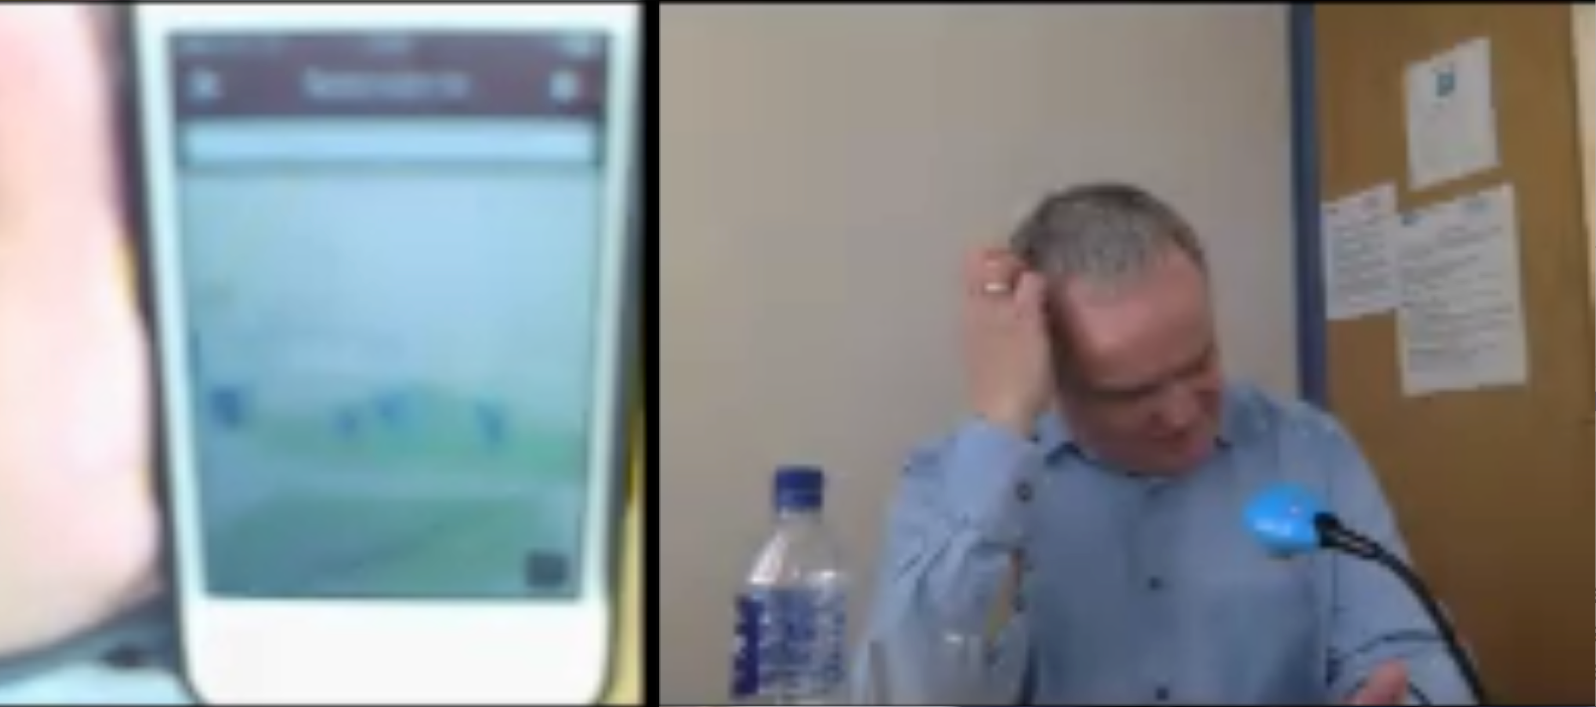
\includegraphics[width=0.7\textwidth]{combined2}
    \caption{One blind tester struggles to navigate a map of bus stops in the Lothian Buses app}
\end{figure}

Each session lasted approximately one hour, and took place either in the RNIB offices in Hillside Crescent, Edinburgh, or in other locations convenient for the testers.

After the cooperative evaluation, the tester completed a survey consisting of nine questions designed to give an insight into various aspects of their experience with each app. Each question took the form of a positive statement about the app, and the tester was asked to provide a level of agreement with the statement (the options being "disagree", "somewhat disagree", "neutral", "somewhat agree", and "agree").

The majority of the statements were concerned with the usability of the app (for example "I found the app easy to use", "The language used in the app is clear", or "I felt confident using the app"). Others were concerned with functionality ("The app does everything I'd expect it to").

There was also a statement regarding the tester's perceived utility of the app: "If using the bus service, I would use this app". It was assumed that blind or partially-sighted testers would be more likely to agree with this statement when discussing the Talking Buses app, and that sighted users would be more likely to agree when discussing the Lothian Buses app.

\subsubsection{Results}
Note that when discussing the quantitative results for each task, we refer to average task completion time or average number of errors made. In calculating these averages, only the results from blind and partially-sighted test users are considered. 

\textbf{Task 1: Find bus service information from nearby bus stops}

Average completion time for the first task was 15 seconds for the Talking Buses app, and 25 seconds for the Lothian Buses official app. None of the test users made any errors using the Talking Buses app, but users experienced several issues with the Lothian Buses app.

One issue was that the names (and thus VoiceOver descriptions) of elements did not correspond to their functionality. There are two elements on the home screen of the Lothian Buses app with names that indicate similar functionality: one, a button labelled "Buses Near Me", the other a list header labelled "Nearby Bus Stops". All but one of the test users commented on this ambiguity. Two of the testers chose the first button, and were taken to a map of bus stops (not, as the label's title suggests, a map of \textit{buses}).

Both of the users who encountered this map experienced several issues. It was clear from their comments and interaction with the app that they had not realised they were viewing a list of stops in a map format. VoiceOver dictation was progressing from left-to-right, top-to-bottom across the map: an unintuitive navigation order for a user who is unable to actually perceive the map as intended. Both of the users who chose the "Buses Near Me" button eventually became stuck and asked for assistance. Had the "Buses Near Me" button had an appropriate accessibility hint, users would have known this was not the correct option and could have avoided the map altogether.

All users eventually located the list of nearby bus stops. As mentioned above, this list contained a header item, with a text label "Nearby Bus Stops". The header contained very little accessibility information (its VoiceOver description simply stated "Nearby Bus Stops", without giving any other explanation). Several test users assumed it was an incorrectly annotated button, and attempted to select it. Again, correct usage of VoiceOver accessibility attributes would have prevented this.

Two of the test users were curious about the "Main Menu" button at the top-left corner of the home screen. One asked "If this is the home screen, why do we need a main menu?". The other commented on the lack of VoiceOver hint, and explained that he would now have to explore either the entire menu, or the entire user-interface as the description supplied had given him no new information.

When users were dictated information on the nearby bus stops, several were confused by the uncorrected abbreviation of the bus stop's heading (one user interpreted the "N" representing "North" as the word "end"), and in one case the tester had to make VoiceOver repeat the information several times to be sure of the stop's description.

In contrast, test users were positive about the experience of completing this task in the Talking Buses app. They agreed that the information supplied by VoiceOver for each element was sufficiently descriptive, and that they could easily predict the outcome of activating them. One of the testers described the user interface as "a really nice screen!", another commented on the "simple clarity" of the layout of elements.


\textbf{Task 2: Find out when the next bus leaves for a particular service from a nearby bus stop}

When using the Talking Buses app, test users completed this task, on average, in 16 seconds, compared to an average of 23 seconds with the Lothian Buses app. This increase in task completion time was largely due to a single design decision: an element providing weather information located above the list of incoming bus services.

Every user initially paused to listen to the description of this element, before realising that it was not useful information for completing the task and moving on. Two of the users noticed that the contents of the element updated over time, and paused, assuming the bus service information would follow. A more thorough application of Apple's VoiceOver guidelines could have prevented this unnecessary delay for the user.

This issue is also caused by an ordering of user-interface elements which does not correspond to the relative importance of these elements. For completing the task that this screen is designed for, the departure times of the buses at the selected stop have more value that the current weather.

Several users commented on the lack of an adequate description for the "Back" button at the top-left of many screens in the Lothian Buses app (it provides the VoiceOver dictation "Go Back. Button."). When using standard user-interface elements, the Back button's description is automatically set to include the title of the previous screen (for example, in the Talking Buses app, after the user has selected a bus service for which to received arrival updates, the description of the "Back" button on the following screen is "Next Buses. Back button."). When asked to clarify why this was important, users stated that it helped them maintain a context of "where I am in the app". One user commented "Go Back. Button. Go back to what?".


\textbf{Task 3: Find out the next three bus stops this service calls at, and their estimated times of arrival}

This task took an average of 22 seconds to complete using the Talking Buses app, and an average of 34 seconds using the Lothian Buses app. There were several reasons for this difference, and a number of other minor accessibility issues with the Lothian Buses app.

Due to the layout of the elements on the relevant screen in the Lothian Buses app, a VoiceOver user must scroll past a number of incoming buses for the selected service, as well as a button and a list header, before they reach information on the bus's route and arrival time at bus stops.

Additionally, the list of bus services that the user must scroll through does not supply a VoiceOver hint attribute, so the result of activating one of the list items is not intuitive. Several users double-tapped when a service was selected, assuming the app would then supply them with route information, but were disappointed when the app simply read the bus service description again.

After scrolling past the list of bus services, two users selected the "Route map" button, and were presented with a map showing the bus route. When asked about their action, these users explained that they had assumed the route information would be given in a format besides a map (it was not). One of these users said that they had taken the chance because they were not confident in their understanding of the user interface, and wanted to be thorough in their exploration.

All test users eventually found the list of bus stops on the route, and their estimated arrival times. Several of the users attempted to scroll through the list of bus stops by dragging their finger down, and were surprised to find how vertically small the items were. They described selecting a specific bus stop as "tricky". VoiceOver users who navigated the list using swipe gestures did not experience this issue.

\begin{figure}[h!]
  \centering
    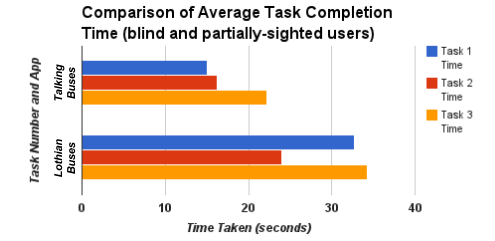
\includegraphics[width=0.9\textwidth]{chart_1}
    \label{fig:chart1}
\end{figure}

\begin{figure}[h!]
  \centering
    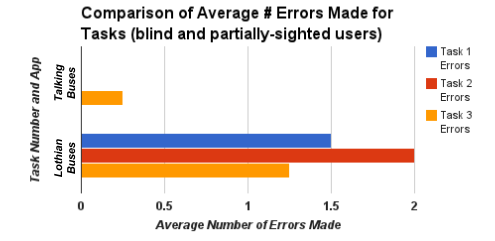
\includegraphics[width=0.9\textwidth]{chart_2}
    \label{fig:chart2}
\end{figure}

\subsubsection{Summary}

Overall, the quantitative data collected during the cooperative evaluation suggests that the Talking Buses app is more accessible to blind and partially-sighted users than the Lothian Buses official app. The average time taken to complete tasks was lower for all tasks for the Talking Buses app, as was the number of errors made by test users.

Additionally, test users identified a number of accessibility issues with the Lothian Buses official app that were not present in the Talking Buses app. Most issues identified by users were caused by an incorrect or incomplete implementation of VoiceOver. Other issues largely concerned the ordering of user-interface elements, and aspects of the visual design of the user interface, such as the sizing of elements.

\textbf{Qualitative Results - User Survey:}

The responses to the qualitative statements are included in Figure \ref{fig:heatmap}. In this table, users one through three are blind, user four is partially-sighted, and users five and six are sighted users. Responses are converted into numerical labels, a "1" representing "disagree", "4" representing "somewhat disagree", and so on. These responses are also colour coded, allowing for general trends to be identified more easily. The average response for each statement is also shown in Figure \ref{fig:chart3}.

\begin{figure}[h!]
\label{heatmap}
  \centering
    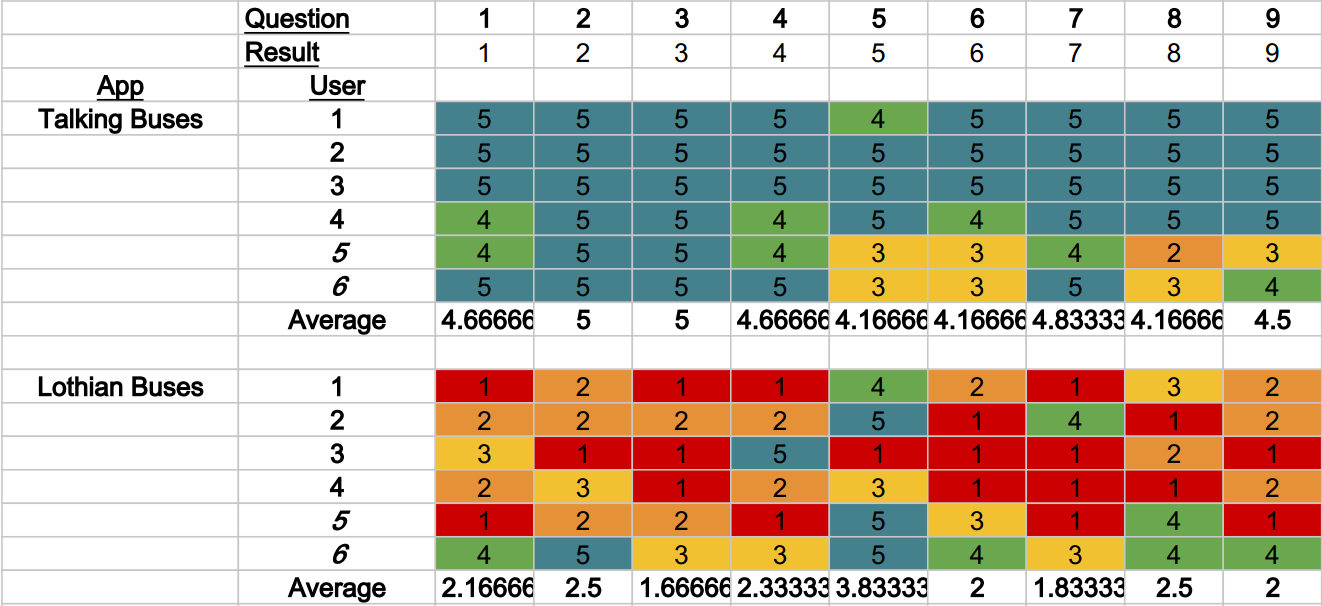
\includegraphics[width=\textwidth]{heatmap}
    \caption{Showing average responses to each question in the post-evaluation survey, designed to qualitatively gauge user experience}
    \label{fig:heatmap}
\end{figure}

\begin{figure}[h!]
  \centering
    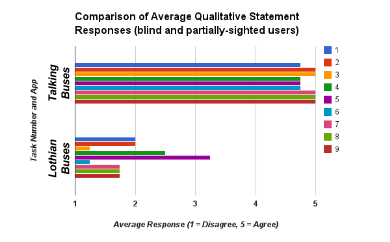
\includegraphics[width=\textwidth]{chart_3}
    \caption{A colour-coded table of individual responses to the post-evaluation survey}
    \label{fig:chart3}
\end{figure}

For every positive statement, test users were significantly more likely to agree when talking about the Talking Buses than when talking about the Lothian Buses official app. For five of the nine statements, all test users responded "Agree". 

The two statements test users disagreed with most when discussing the Lothian Buses official app were "The language used in the app is clear.", and "The app works the way I expected it to.", reflecting issues identified with VoiceOver attributes and pronunciation, and ambiguity over how functionality was accessed by the user.

The Lothian Buses official app performed best when discussing functionality: three out of the six user agreed with the statement "The app does everything I'd expect it to" (though two of these test users were sighted users). The Lothian Buses official app offers a wide variety of additional functionality besides providing essential bus service information, including pre-paid mobile ticketing.

The Talking Buses app performed similarly for this statement, perhaps indicating that the functionality implemented performs assists blind and partially-sighted users in the tasks most demanding of aid.

Two notable differences were observed in the responses of the sighted users compared to the blind and partially-sighted users. Sighted users were more likely to agree with the statement: "The app does everything I'd expect it to" with the Lothian Buses app than for the Talking Buses app. This likely reflects their prior experience with bus travel apps such as EdinBus, which cover a wider range of functionality, much of which is included in the Lothian Buses official app.

Additionally, sighted users were more likely to agree with the statement "If using the bus service, I would use this app" with the Lothian Buses official app than with the Talking Buses app (one "somewhat disagree" and one "neutral" response compared to two "somewhat agree" responses). Again, this is explained by the potential for these users to use a more functional solution, as it is accessible to them (unlike for blind and partially-sighted users).

\section{Conclusions and Discussion}
\subsection{Conclusions}
This project has created Talking Buses, a smartphone application allowing blind and partially-sighted bus users to access bus service information through a system of spoken location and journey updates. Additionally, the project has created a server component capable of fetching, processing and serving bus service information to the iPhone app.

The app was designed according to a series of design principles intended to cater for blind and partially-sighted users, and iteratively developed using feedback from a series of meetings with the RNIB Mobile User Group. It is capable of supporting blind and partially-sighted people in many tasks associated with bus travel, from planning a journey to tracking the progress of a bus in real time.

The Talking Buses app was evaluated using a heuristic evaluation conducted by the designer, and a cooperative evaluation involving four blind and partially-sighted smartphone users, and two sighted users. The app was evaluated in comparison to the Lothian Buses app (an app offering additional functionality, but not specifically designed for blind and partially-sighted users).

The heuristic evaluation identified a number of issues with the Lothian Buses official app not present in the Talking Buses app. Many of these issues involved aspects of visual design (specifically the layout applied to elements, and the size of text displayed to the user). Other issues concerned the annotation of user interface elements with appropriate accessibility attributes, with a predicted detrimental affect on the user's experience. None of these issues were identified in the Talking Buses app.

Many of these issues were confirmed by users during the cooperative evaluation. Other issues identified included a counter-intuitive ordering of elements in the user interface, and ambiguous use of language in VoiceOver descriptions of elements. Again, these issues were not identified during testing with the Talking Buses app.

A survey (included in \ref{appendA}) was conducted to collect qualitative data on the user's experience, by measuring a level of agreement with a series of positively-worded statements. In all statements, users were more likely to agree when discussing the Talking Buses app than when discussing the Lothian Buses app.

Understandably, sighted users were more likely to agree that the Lothian Buses app offered all the functionality they expected, and that they would be more likely to use the Lothian Buses app in the future. As discussed, this is to be expected - the Lothian Buses official app is accessible to sighted users.

Mobile applications created specifically for blind and partially-sighted users can be expected to have different design goals from those designed for the average user. Understandably, this can result in these applications having a significantly different appearance (for example, using larger fonts or a limited range of colours).  

However, such fragmentation can also have a detrimental effect on user experience. This project has demonstrated the availability of resources which aim to support developers in creating mobile applications which are accessible to blind and partially-sighted users. It is the belief of the author that many of the principles and strategies provided could be applied to the majority of existing mobile applications without negatively impacting the experience of sighted users.

Several areas for future development were identified at the end of the project. Several bus services in Edinburgh now offer on-board Wi-Fi connections, providing users with a fairly reliably internet connection during bus journeys \citep{lothianWiFi}. In order to provide this, the bus service has a greater bandwidth than a standard bus, and could potentially use this bandwidth to transmit its current location to the MyBusTracker API on a much more frequent basis. This, combined with a period of GPS data collection on the iPhone, could allow for the automatic identification of the bus a user is currently travelling on.

The development of the tram service has been an area of much discussion in Edinburgh since construction began in 2007, and their testing was carried out during the writing of this dissertation. Much of the information provided to the users by the Talking Buses app regarding bus service information will presumably also apply to tram services. If information (including real-time service information) on the new tram services is supplied by the MyBusTracker API, it would be very simple to adapt the app for use with the tram service, allowing blind and partially-sighted users to take advantage of its accessibility when using the trams.

With the increase in availability of high-speed mobile internet connection in cities, there could be the potential for information to be exchanged between the passengers and the drivers of bus services. For example, a blind or partially-sighted bus user waiting at a bus stop could use the app to signal their intention to board to the bus driver of a specific bus service. When approaching the bus stop, the driver would receive a notification that a blind or partially-sighted passenger had requested the bus service, and would know to stop without any action required from the passenger.

Overall, blind and partially-sighted users who used the app at various stages in its development were hugely enthusiastic about the project, and expressed gratitude for taking the time to make an accessible solution to a challenging task.

% Appendix
\appendix
\section*{APPENDIX}
\appendixhead{Wait}

% Acknowledgments
\begin{acks}
First, I wish to express gratitude to the Royal National Institute for the Blind, and in particular the members of the Mobile User Group in Edinburgh. Their perspective and feedback were an invaluable contribution to the app, and our meetings proved to be one of the most enjoyable aspects of the project.

Secondly, I wish to thank my supervisor, Professor Stephen Gilmore, for supporting me throughout the project. Stephen's patience and pragmatism are among the main reasons the project achieved its goals.

Additionally, I would like to thank Stuart Lowrie and Gary Wilson from Edinburgh Council for providing access to the MyBusTracker API for the project, as well as Niall Scott and Gordon Christie (the developers of the My Bus Edinburgh and EdinBus apps) for their continued support in working with the API.

I'd like to thank Gavin Dutch from Kotikan for use of their video recording equipment during the cooperative evaluation, and Gavin Neate from Neatebox for much useful advice on building products for the blind and partially-sighted community.

Lastly, I'd like to thank all of my friends and family who gave feedback on the app at various stages of the design (especially the earlier ones), and for their continued support and camaraderie over the past five years.
\end{acks}

% Bibliography
\bibliographystyle{ACM-Reference-Format-Journals}
\bibliography{mybibfile}
                             % Sample .bib file with references that match those in
                             % the 'Specifications Document (V1.5)' as well containing
                             % 'legacy' bibs and bibs with 'alternate codings'.
                             % Gerry Murray - March 2012

% History dates
\received{June 2014}{June 2014}{June 2014}

% Electronic Appendix
\elecappendix

\medskip

\section{Evaluation Survey}
\label{appendA}
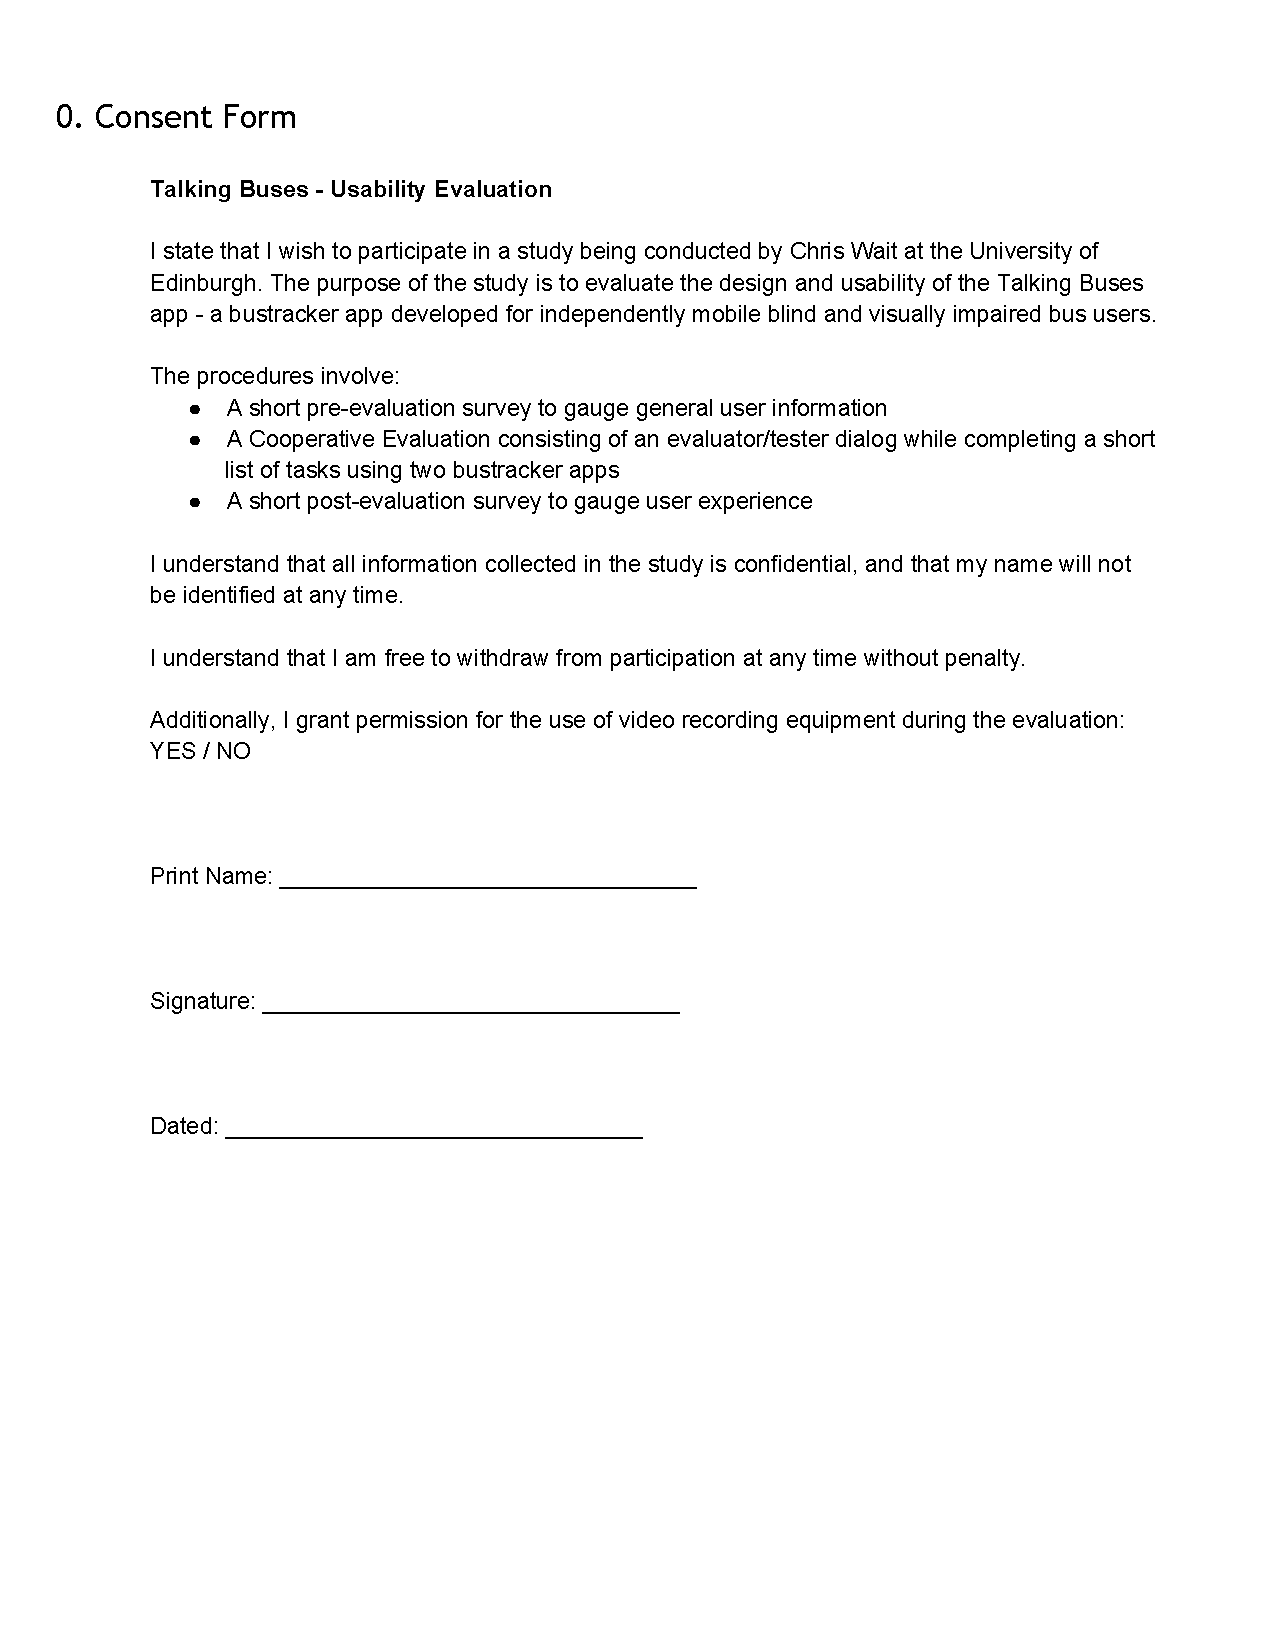
\includepdf[pages={1-},scale=0.75]{Survey.pdf}

\section{Use Cases}
\label{sec:useCases}
Use cases are defined as "a goal-oriented set of interactions between external actors and the system under consideration", and are widely recognised in software development as a useful tool for extracting functional requirements for a system \citep{useCases}.  In order to inform the specification for the functionality of the system, a number of potential use cases were considered.

In the case of this project, the system includes both the Talking Buses app and associated server component.  For each use case, the primary actor is a blind or partially-sighted bus user. Use cases which require real-time bus service information include a secondary actor: the MyBusTracker API.

\textbf{Use Case 1: "Find information on nearby bus stops"}

\textbf{Main Success Scenario}:
\begin{easylist}[enumerate]
& The user opens the app. 
& The app checks to see if it has a local database of bus stops.
&& If the app does not find a local database of bus stops, it downloads one from the server component, and stores the topology ID.
&& If the app does find a local database of bus stops, its topology ID is compared to that held by the server component.
&&& If the server component has a different (and therefore newer) topology ID than the one held by the app, the app downloads the new database of bus stops from the server component.
&&& Otherwise, the locally stored database is up-to-date, and the app continues execution.
& The app finds the user's location and presents a list of bus stops located near the user, sorted from closest to furthest away.
& The user explores this list of items attempting to find appropriate bus stop(s).
&& For each bus stop explored by the user, the app provides the bus stop name, its heading, and a list of the bus services which call at the stop.
\end{easylist}

\textbf{Use Case 2: "Find bus departures from a nearby bus stop"}

Here we assume that the user has identified a nearby bus stop for which they wish to receive information on departures, as per stage three of Use Case 1.

\textbf{Main Success Scenario}:
\begin{easylist}[enumerate]
& The user selects the desired bus stop from the list.
& The app requests real time information on bus services due to arrive at the chosen bus stop from the MyBusTracker API.
& Once this information is received, the app presents a list of bus services, sorted by service mnemonic from lowest to highest.
& The user explores this list of items attempting to find appropriate bus service.
&& For each bus service explored by the user, the app provides the service mnemonic, destination and estimated time(s) of arrival.
\end{easylist}

\textbf{Use Case 3: "Receive updates on arrival times for a selected bus service"}

Here we assume that the user has selected a nearby bus stop from which they wish to depart (Use Case 1) and that they have also identified a bus service which they wish to use, as per stage 3 of Use Case 2.

\textbf{Main Success Scenario}:
\begin{easylist}[enumerate]
& The user selects the desired bus service from the list.
& The app begins to frequently request updates on the estimated arrival time of the desired bus service from the MyBusTracker API.
& When these updates are received, the app dictates the new estimated arrival time, in minutes, to the user. The app also populates the user interface with information on the bus service (the same information provided on the previous screen).
\end{easylist}

\textbf{Use Case 4: "Receive updates on estimated arrival times at bus stops for a bus service"}

Here we assume that the user has selected a nearby bus stop from which they wish to depart (Use Case 1) and that they have also identified a bus service which they wish to use, as per stage 3 of Use Case 2. We also assume that they have selected the Show Route button (either after boarding the bus, or while planning a bus journey).

\textbf{Main Success Scenario}:
\begin{easylist}[enumerate]
& The user selects the Show Route button on the Waiting For Bus screen.
& The app begins to frequently request updates on the estimated arrival time of the chosen bus service at bus stops on its route.
& When these updates are received, the app presents them to the user. For each bus stop, the app dictates the bus stop name, its heading, and the estimated arrival time in minutes.
\end{easylist}

\section{Server Component Update Process}
In order to ensure that the app is able to provide high-quality, relevant information to users, steps must be taken to ensure the information held in the Talking Buses database is as accurate and up-to-date as possible. To accomplish this, a process was devised by which the server component manages its own updates on a regular basis. We now describe this process.
\begin{easylist}[enumerate]
& Once weekly, at a predefined time, the update process starts.
&& A cron job calls a python script responsible for handling the update process.
& First, the server checks to see if it must be updated.
&& We store the current topology id of the information available from the MyBusTracker API. If this has changed since we last checked, the database will be updated.
\end{easylist}

If the database does require updating:
\begin{easylist}
& The latest NaPTAN CSV dump from data.gov.uk is downloaded. This file is relatively large (around 197 Megabytes uncompressed), and so steps are taken to minimise unnecessary computation:
&& A single file (Stops.CSV) is extracted, containing information on bus stops in the UK. This file is around 130 Megabytes in size.
&& Rows containing bus stops in the Edinburgh and Midlothians areas are extracted, and stored in a separate file. By this point the file has reached 1.2 Megabytes in size, and the unnecessary NaPTAN data is removed from the server.
& The latest data from the MyBusTracker API is downloaded in JSON format.
&& Bus stops, bus services, and destinations are parsed and then stored in the database.
& Bus stops from the MyBusTracker API are augmented with information from NaPTAN.
&& This additional information includes the street name and bus stop name.
& The number of bus stops without information from NaPTAN is calculated.
& The new topology id from the MyBusTracker API is stored.
& Finally, a log of the update process is stored and sent to a predefined email address for the system administrator.
\end{easylist}

\begin{figure}[h!]
  \centering
    \fbox{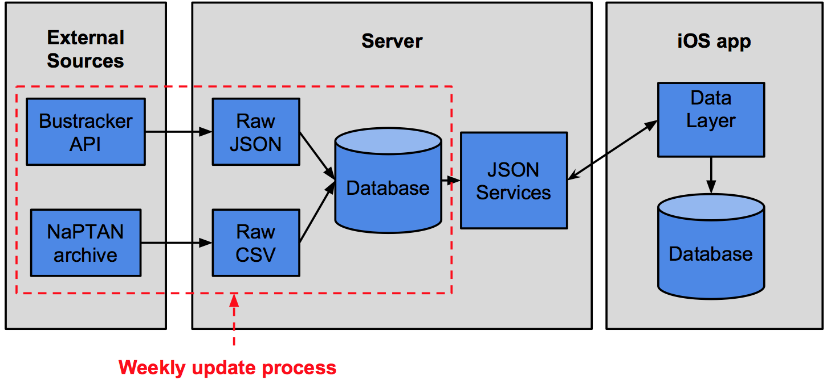
\includegraphics[width=\textwidth]{updateArch}}
    \caption{A diagram showing the architecture of the new database update process}
\end{figure}

\section{iOS Bus Stop Storage - CoreData}
At this stage in the project, the decision was made to reimplement the method of storing the local database of bus stops in the Talking Buses app. The original solution of storing the database of stops using a property list file was intended as a temporary one, and there are many advantages to using the CoreData framework to handle persistent storage of objects in an iOS application. We review features of the CoreData framework, details of the implementation, and the advantages of having done so.

CoreData is designed to provide "generalized and automated solutions to common tasks associated with object life-cycle and object graph management, including persistence" \citep{coreData}. This means that it provides a layer of abstraction for making objects persistent, and handles the relationships between these persistent objects. CoreData provides a variety of features, and we now give an overview of these:
\begin{easylist}[itemize]
& CoreData provides tools to simplify migrations to the schema used to define persistent objects. This makes supporting changes to the information stored on each bus stop in the Talking Buses system an easier task, making the project more maintainable.
& CoreData provides a method of developing complex queries using instances of the NSPredicate class. This removes the need to write complex queries in SQL to retrieve objects from the local database, and supports a wide range of functions including the sorting of results and searching using regular expressions.
& CoreData provides support for tracking and undoing changes made to persistent data. While this functionality was not deemed to be necessary for the implementation of the functionality in the Talking Buses iPhone application, there are many potential future features to which it applies.
\end{easylist}

The XCode integrated development environment simplifies the process of adding support for CoreData to an existing project, allowing for rapid integration in the Talking Buses app. Once the CoreData framework has been added to the project, the developer creates a managed object model. This model provides a schema detailing the attributes stored for different entities (objects managed using CoreData). XCode provides the Data Model Design tool, designed to simplify the process of populating this managed object model with entities and configuring attributes for these entities. 

\begin{figure}[h!]
  \centering
    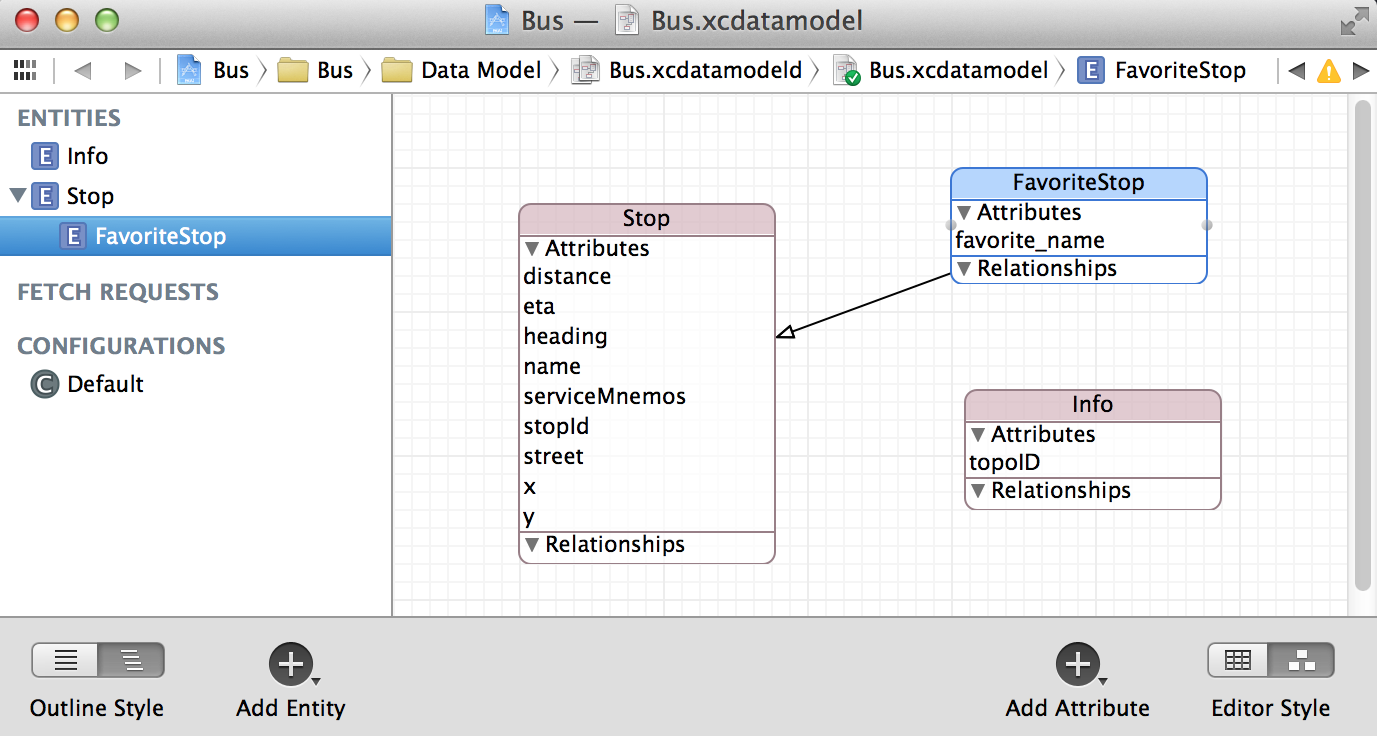
\includegraphics[width=0.8\textwidth]{dataModelDesigner}
    \caption{Defining the CoreData Managed Object Model, using Xcode's Data Model Design tool}
\end{figure}

A managed object model was created and populated with entities representing bus stops, favourite bus stops (a subclass of bus stops), and an info object designed to store the current topology ID held by the Talking Buses app. Additionally, a class was implemented to be represented by each of the entities in the managed object model.

This is not strictly necessary, but can be useful in providing dynamic attributes to an element (attributes for which the value must be evaluated, as opposed to simply being read from the local database). Entity inheritance was used to make the favourite bus stop entity a child of the bus stop entity (to save reimplementing any business logic).

Once the managed object model is configured, an app must create an instance of a managed object context. This is used to maintain all objects managed by CoreData, and any relationships that exist between them. The managed object context acts as a "scratch pad" - that is, it is capable of tracking and undoing changes, and will only write to the persistent store when requested to.

The managed object context writes data to the persistent object store (the abstraction of the database) using a persistent store coordinator (which mediates between the objects in the application, and the database).

An additional advantage of using the CoreData framework, is that it handles much of the responsibility of memory management and concurrency with minimal performance implications (compared to those which may be incurred if implementation of these features was implemented by the developer) \citep{coreData}.

Integration with the CoreData framework was implemented as described above, and the previous solution of storing bus stop data to property lists files disabled and removed from the Talking Buses app.

\end{document}
% End of v2-acmsmall-sample.tex (March 2012) - Gerry Murray, ACM


